\documentclass[12pt]{report}


\usepackage{eqparbox}
\usepackage{mathtools}
\usepackage{amsmath}
\usepackage{amsfonts}
\usepackage{systeme}
\usepackage{siunitx}
\usepackage[T1]{fontenc}
\usepackage{hyperref}
\usepackage{bigfoot}
\usepackage[numbered, framed]{matlab-prettifier}
\usepackage{filecontents}
\usepackage{graphicx}
\hypersetup{
colorlinks,
citecolor=black,
filecolor=black,
linkcolor=black,
urlcolor=black
linkto=all,
}

\newenvironment{simplechar}{%
   \catcode`\^=12
}{}

\title{Numerical Methods, project C, Number 32}
\author{Krzysztof Rudnicki\\ Student number: 307585 \\ Advisor: dr hab. Piotr Marusak}
\date{\today}

\let\ph\mlplaceholder % shorter macro
\lstMakeShortInline"

\lstset{
  style              = Matlab-editor,
  basicstyle         = \mlttfamily,
  escapechar         = ",
  mlshowsectionrules = true,
}

\newcommand\myeq{\mathrel{\overset{\makebox[0pt]{\mbox{\normalfont\tiny\sffamily def}}}{=}}}


\begin{document}
\maketitle
\tableofcontents

\chapter{Determine polynomial function fitting experimental data}
\section{Problem}
Given following samples:
\begin{center}
  \begin{tabular}{| c | c |}
\hline
$x_i$ & $y_i$ \\
\hline
-5 & -6.5743\\
\hline
-4 & 0.9765\\
\hline
-3 & 3.1026\\
\hline
-2 & 1.8572 \\
\hline
-1 & 1.3165 \\
\hline
0 & -0.6144 \\
\hline
1 & 0.1032 \\
\hline
2 & 0.3729 \\
\hline
3 & 2.5327 \\
\hline
4 & 7.3857 \\
\hline
5 & 9.4892 \\
\hline

\end{tabular}
\end{center}

We have to determine polynomial function $ y  = f(x) $ that best fits this data. \\
We will use least-square approximation using system of normal equation with QR factorization.

\section{Theoretical introduction}
\subsection{Linear Least Squares Problem}
We have polynomial function:
\[ y(x) = a_nx^n + a_{n-1}x^{n-1} + \dots + a_1x^1 + a_0 \]
where n - degree of the polynomial we use to approximate function \\
Given matrix $\mathbf{A} \in \mathbb{R}^{m \times n} \quad (m > n)$ and vector $\mathbf{y} \in \mathbb{R}^m$ \\
We need to find vector \^{x} such that:
\[ 	\forall x \in \mathbb{R}^n \quad|| \mathbf{y} - \mathbf{A} \hat{x} ||_2 \leq || \mathbf{y} - \mathbf{A}x ||_2  \]
$\mathbf{A}\hat{x}$ is the vector of values of the approximating function at each data point and $y$ is the vector of values of data points. \\
We have to minimize the Euclidean norm of difference between approximation and data points. \\
To obtain $\hat{x}$ we will calculate the derrivative of error function with respect to $b_n$ and equate it to 0. This way we will get system of equations caled \textbf{normal equations} which have unique solution in form of vector $\hat{x}$

\subsection{Gram matrix and QR decomposition}
We will use Gram's matrix since it's condition number tends to be pretty high which improves the accuracy of our solution. \\
Gram's matrix is a matrix of set of normal equations. The simplest way to present normal equations is by using formula:
\[ \langle \phi_i, \phi_k \rangle \myeq \sum_{j=0}^N \phi_i(x_j)fi_k(x_j) \]
Which then leads to following matrix \textbf{A}:

\[
A = \begin{bmatrix}
\phi_0(x_0) & \phi_1(x_0) &  \dots & \phi_n(x_0) \\
\phi_0(x_1) & \phi_1(x_1) & \dots & \phi_n(x_1) \\
\phi_0(x_2) & \phi_1(x_2) & \dots & \phi_n(x_2) \\
\vdots & \vdots & \vdots & \vdots \\
\phi_0(x_N) & \phi_1(x_N) & \dots & \phi_n(x_N) \\
\end{bmatrix}
\]

In our case we define matrix \textbf{A} as:
\[
A = \begin{bmatrix}
1 & x_0 & (x_0)^2  & \dots & (x_0)^n \\
1 & x_1 & (x_1)^2 &  \dots & (x_1)^n\\
1 & x_2 & (x_2)^2 &  \dots & (x_2)^n\\
\vdots & \vdots & \vdots & \vdots \\
1 & x_N & (x_N)^2 &  \dots & (x_N)^n\\
\end{bmatrix}
\]

Where $x_N$ is the x-axis position for the N-th data point. Then we can express system of natural equations using A in this way:
\[ A^Ty = (A^TA)\hat{x} \]

With condition number of A equal to square root of condition number of Gram's matrix which gives us small errors. It is also usefull for QR factoization since we can rewrite it as follows:
\[ (R^TQ^T)(QR)\hat{x} = (R^TQ^T)y \]
Since determinant of $R \neq 0$ and $Q^TQ = I$ we can simplify aforementioned equation to:
\[ R\hat{x} = Q^Ty \]
And to optimize even further ahead insetead of using QR decomposition we can use faster $\tilde{Q}\tilde{R}$ decomposition:
\[ \tilde{R}\hat{x} = (\tilde{Q}^T\tilde{Q})^{-1}(\tilde{Q}^T) \]
This is faster since $\tilde{R}$ is an upper triangular matrix, easily solved using back-substitution.

\subsection{Gram-Schmidt algorithm}
We will use Gram-Schmidt algorithm for $\tilde{Q}\tilde{R}$ decomposition.
Gram-Schmidt algorithm takes non-orthogonal function basis denoted as:
\[ \phi_0, \dots, \phi_n \]
and orthogonalizes it into orthogonal function basis denoted as:
\[ \psi_0, \dots, \psi_n \]
Standard Gram-Schmid algorithm looks like this:
\[ \psi_0 = \phi_0 \]
\[ \psi_1 = \phi_1 - \frac{\langle \psi_0, \phi_1 \rangle}{\langle \psi_0, \psi_0 \rangle} \psi_0 \]
\[ \psi_n = \phi_n - \sum_{j = 0}^{i-1}  \frac{\langle \psi_j, \phi_i \rangle}{\langle \psi_j, \psi_j \rangle} \psi_j \]
Where $ i = 2, \dots, n $
Then we get a very well conditioned set of normal equations:
\[ a_0\langle \psi_0, \psi_0 \rangle = \langle f, \psi_0 \rangle \]
\[ a_1\langle \psi_1, \psi_1 \rangle = \langle f, \psi_1 \rangle \]
\[ \vdots \]
\[ a_n\langle \psi_n, \psi_n \rangle = \langle f, \psi_n \rangle \]

\section{Results}

I decided to simulate polynomials up to $\mathbf{10^{th}}$ degree.

\begin{center}
   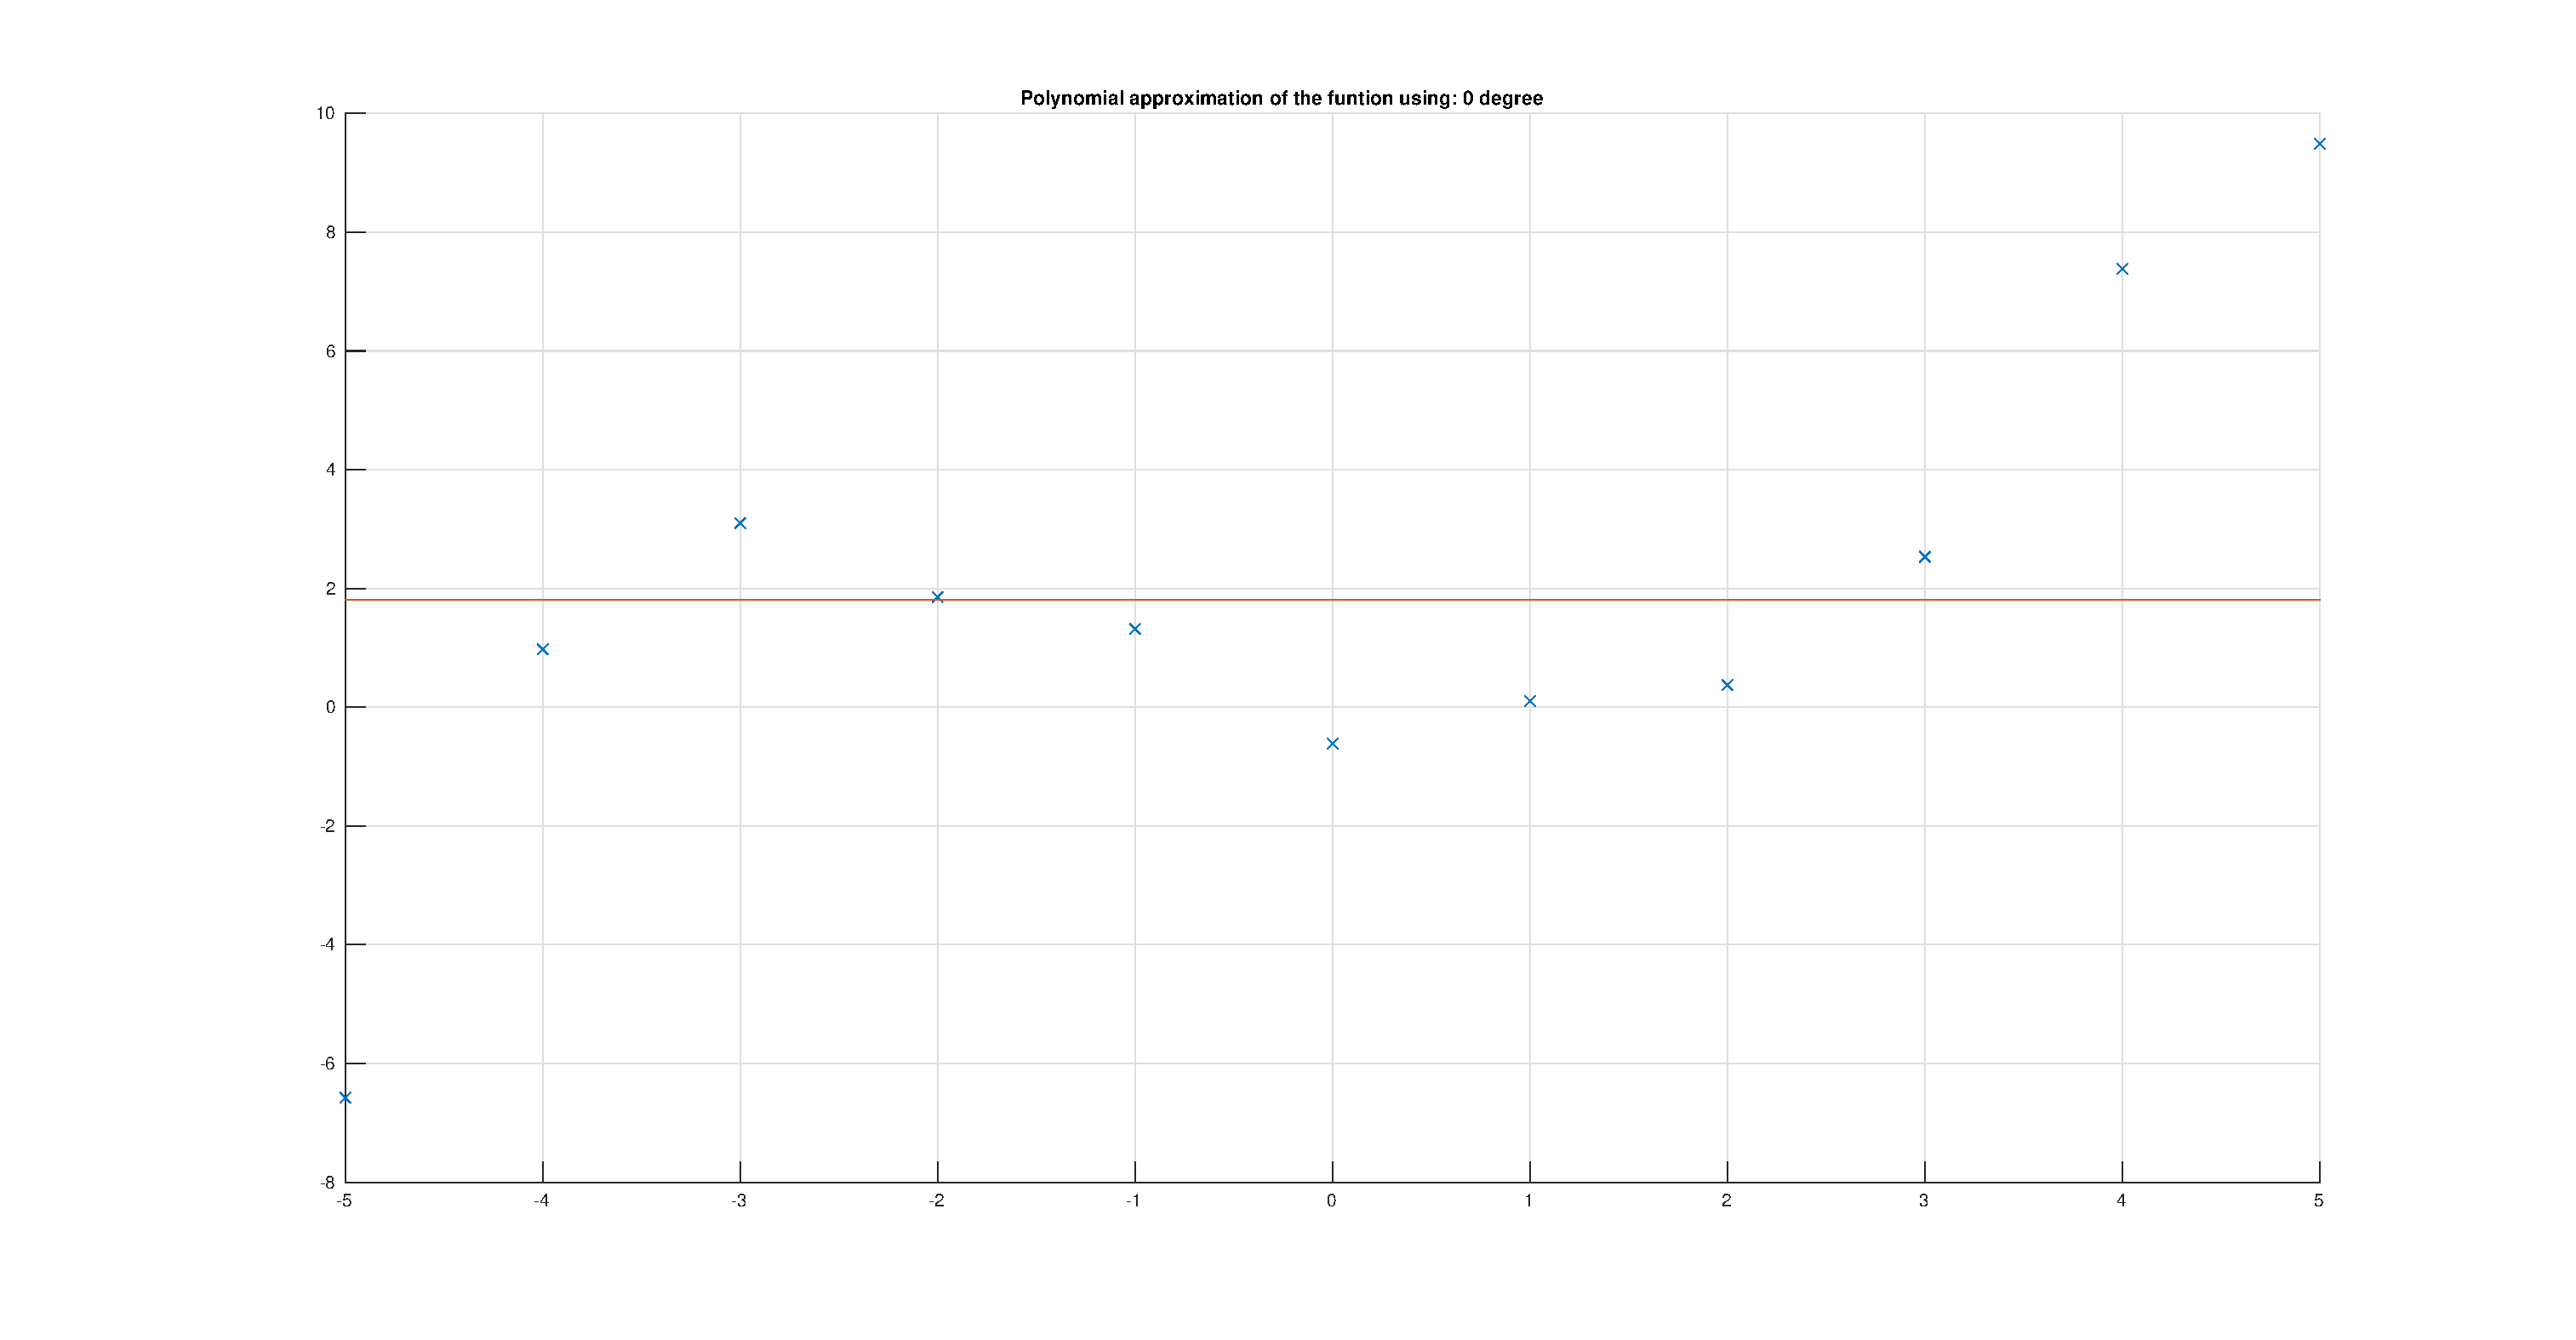
\includegraphics[scale=0.25]{10.eps}
\end{center}

\begin{center}
   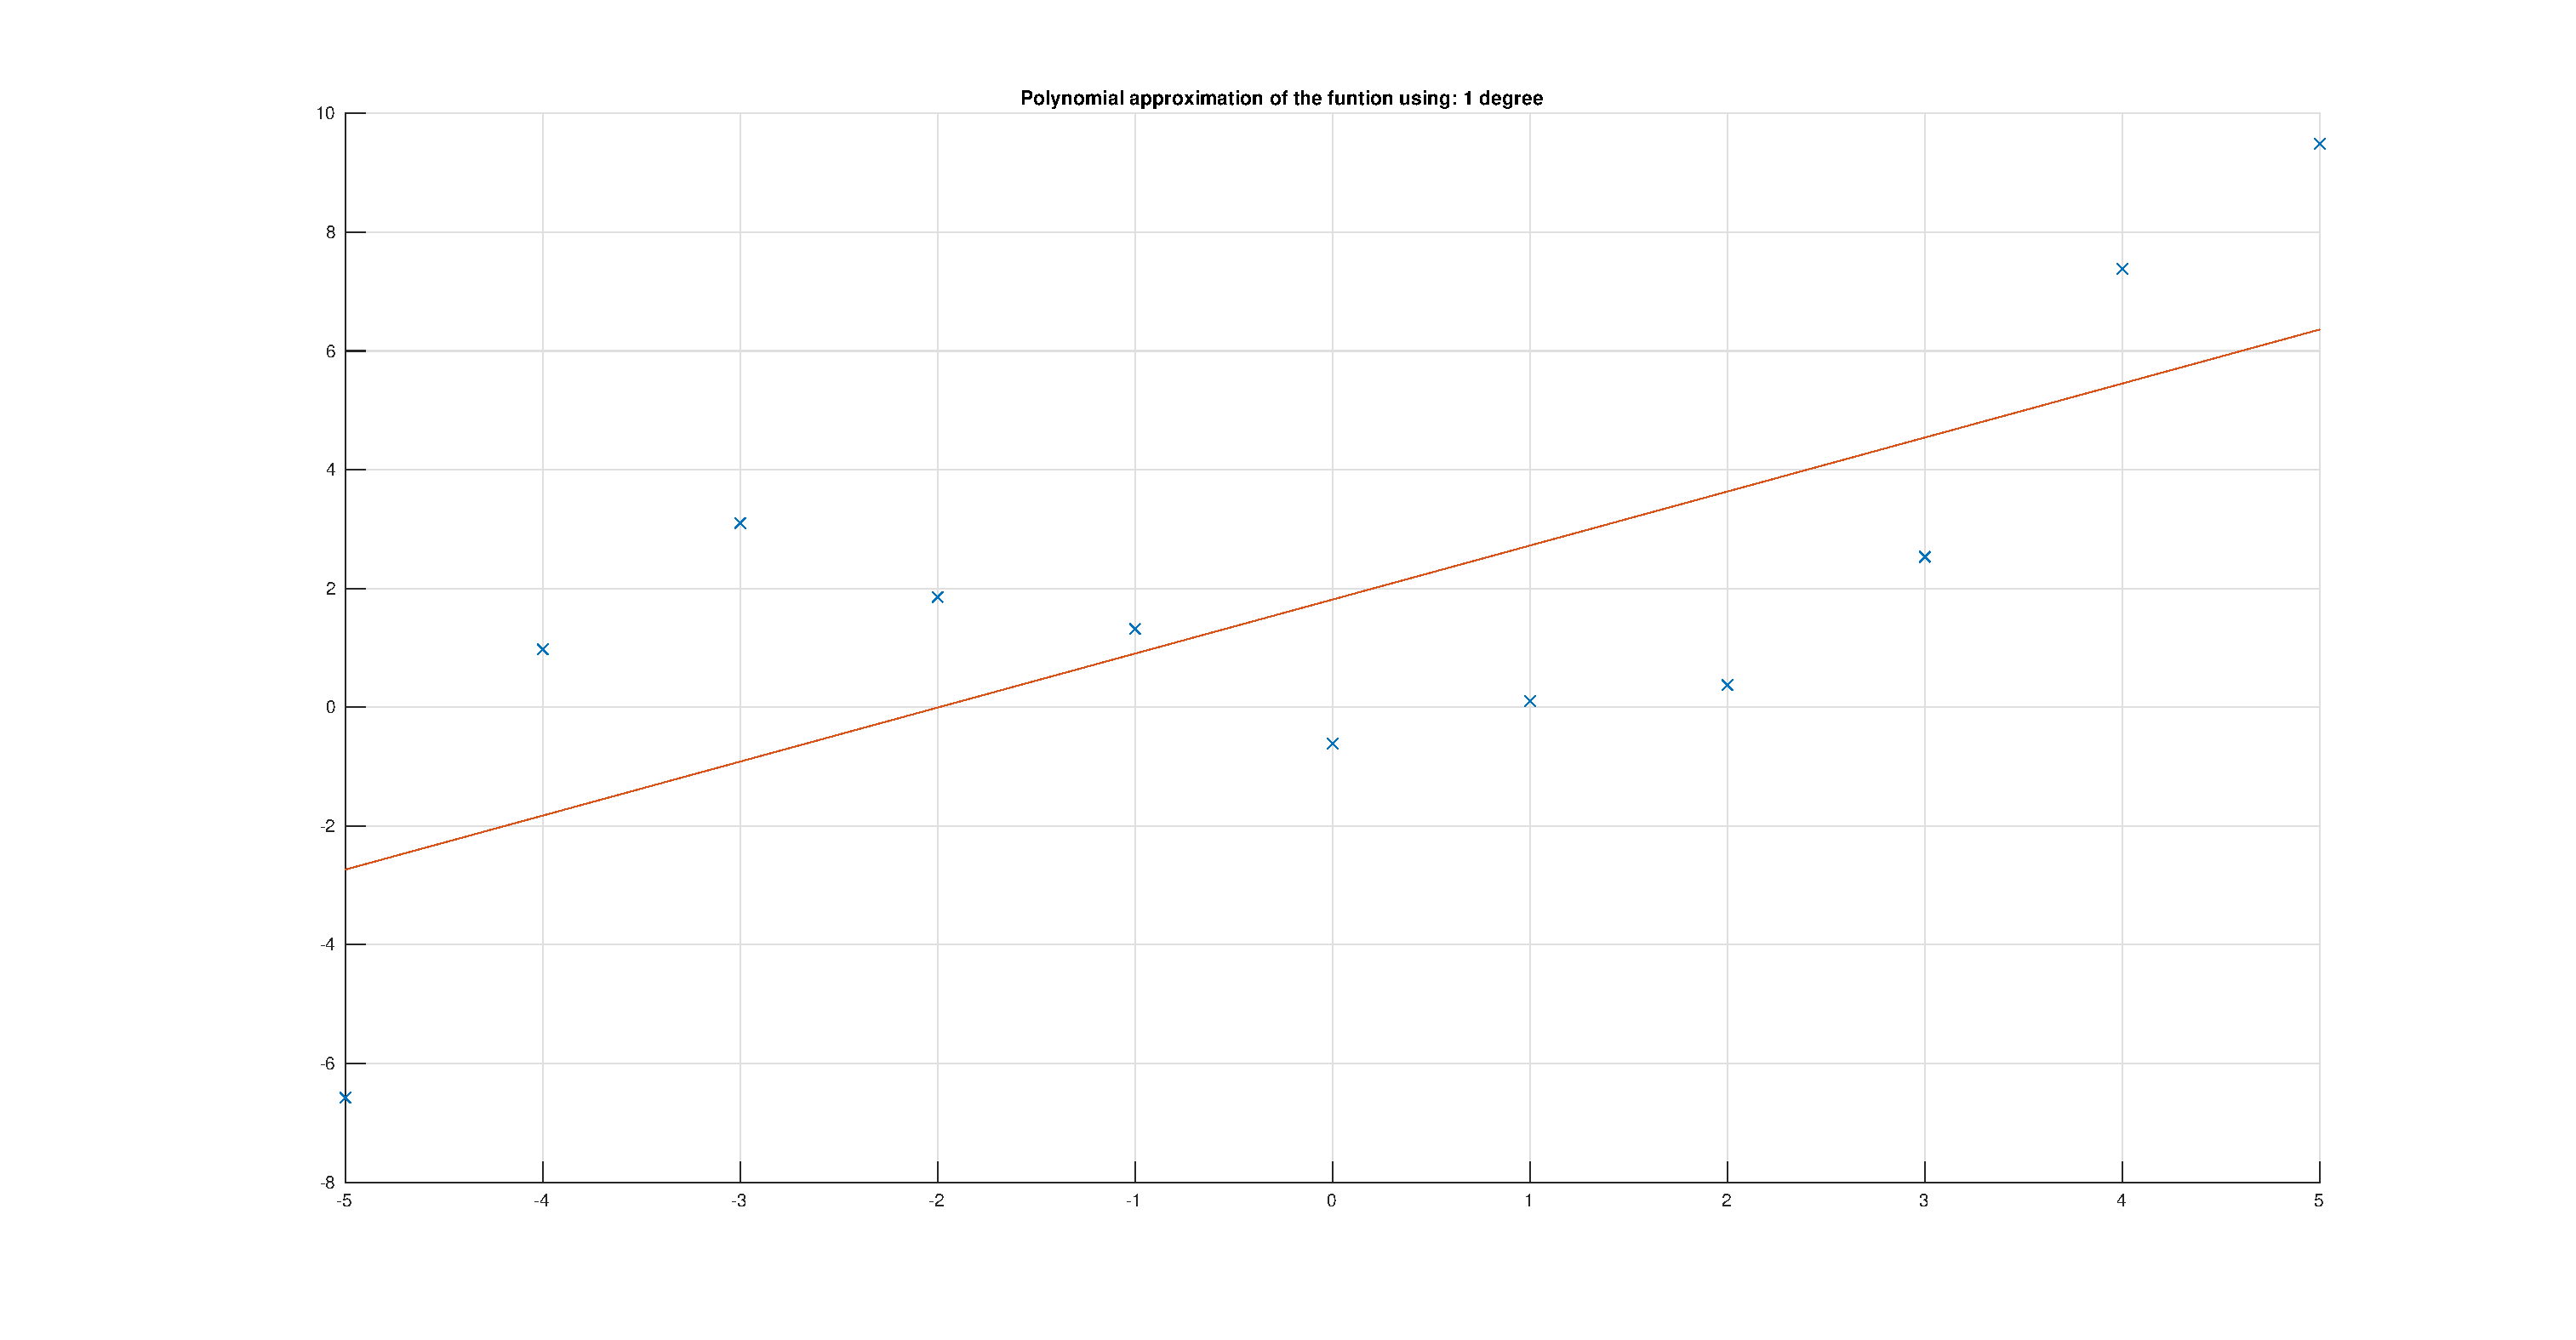
\includegraphics[scale=0.25]{11.eps}
\end{center}

\begin{center}
   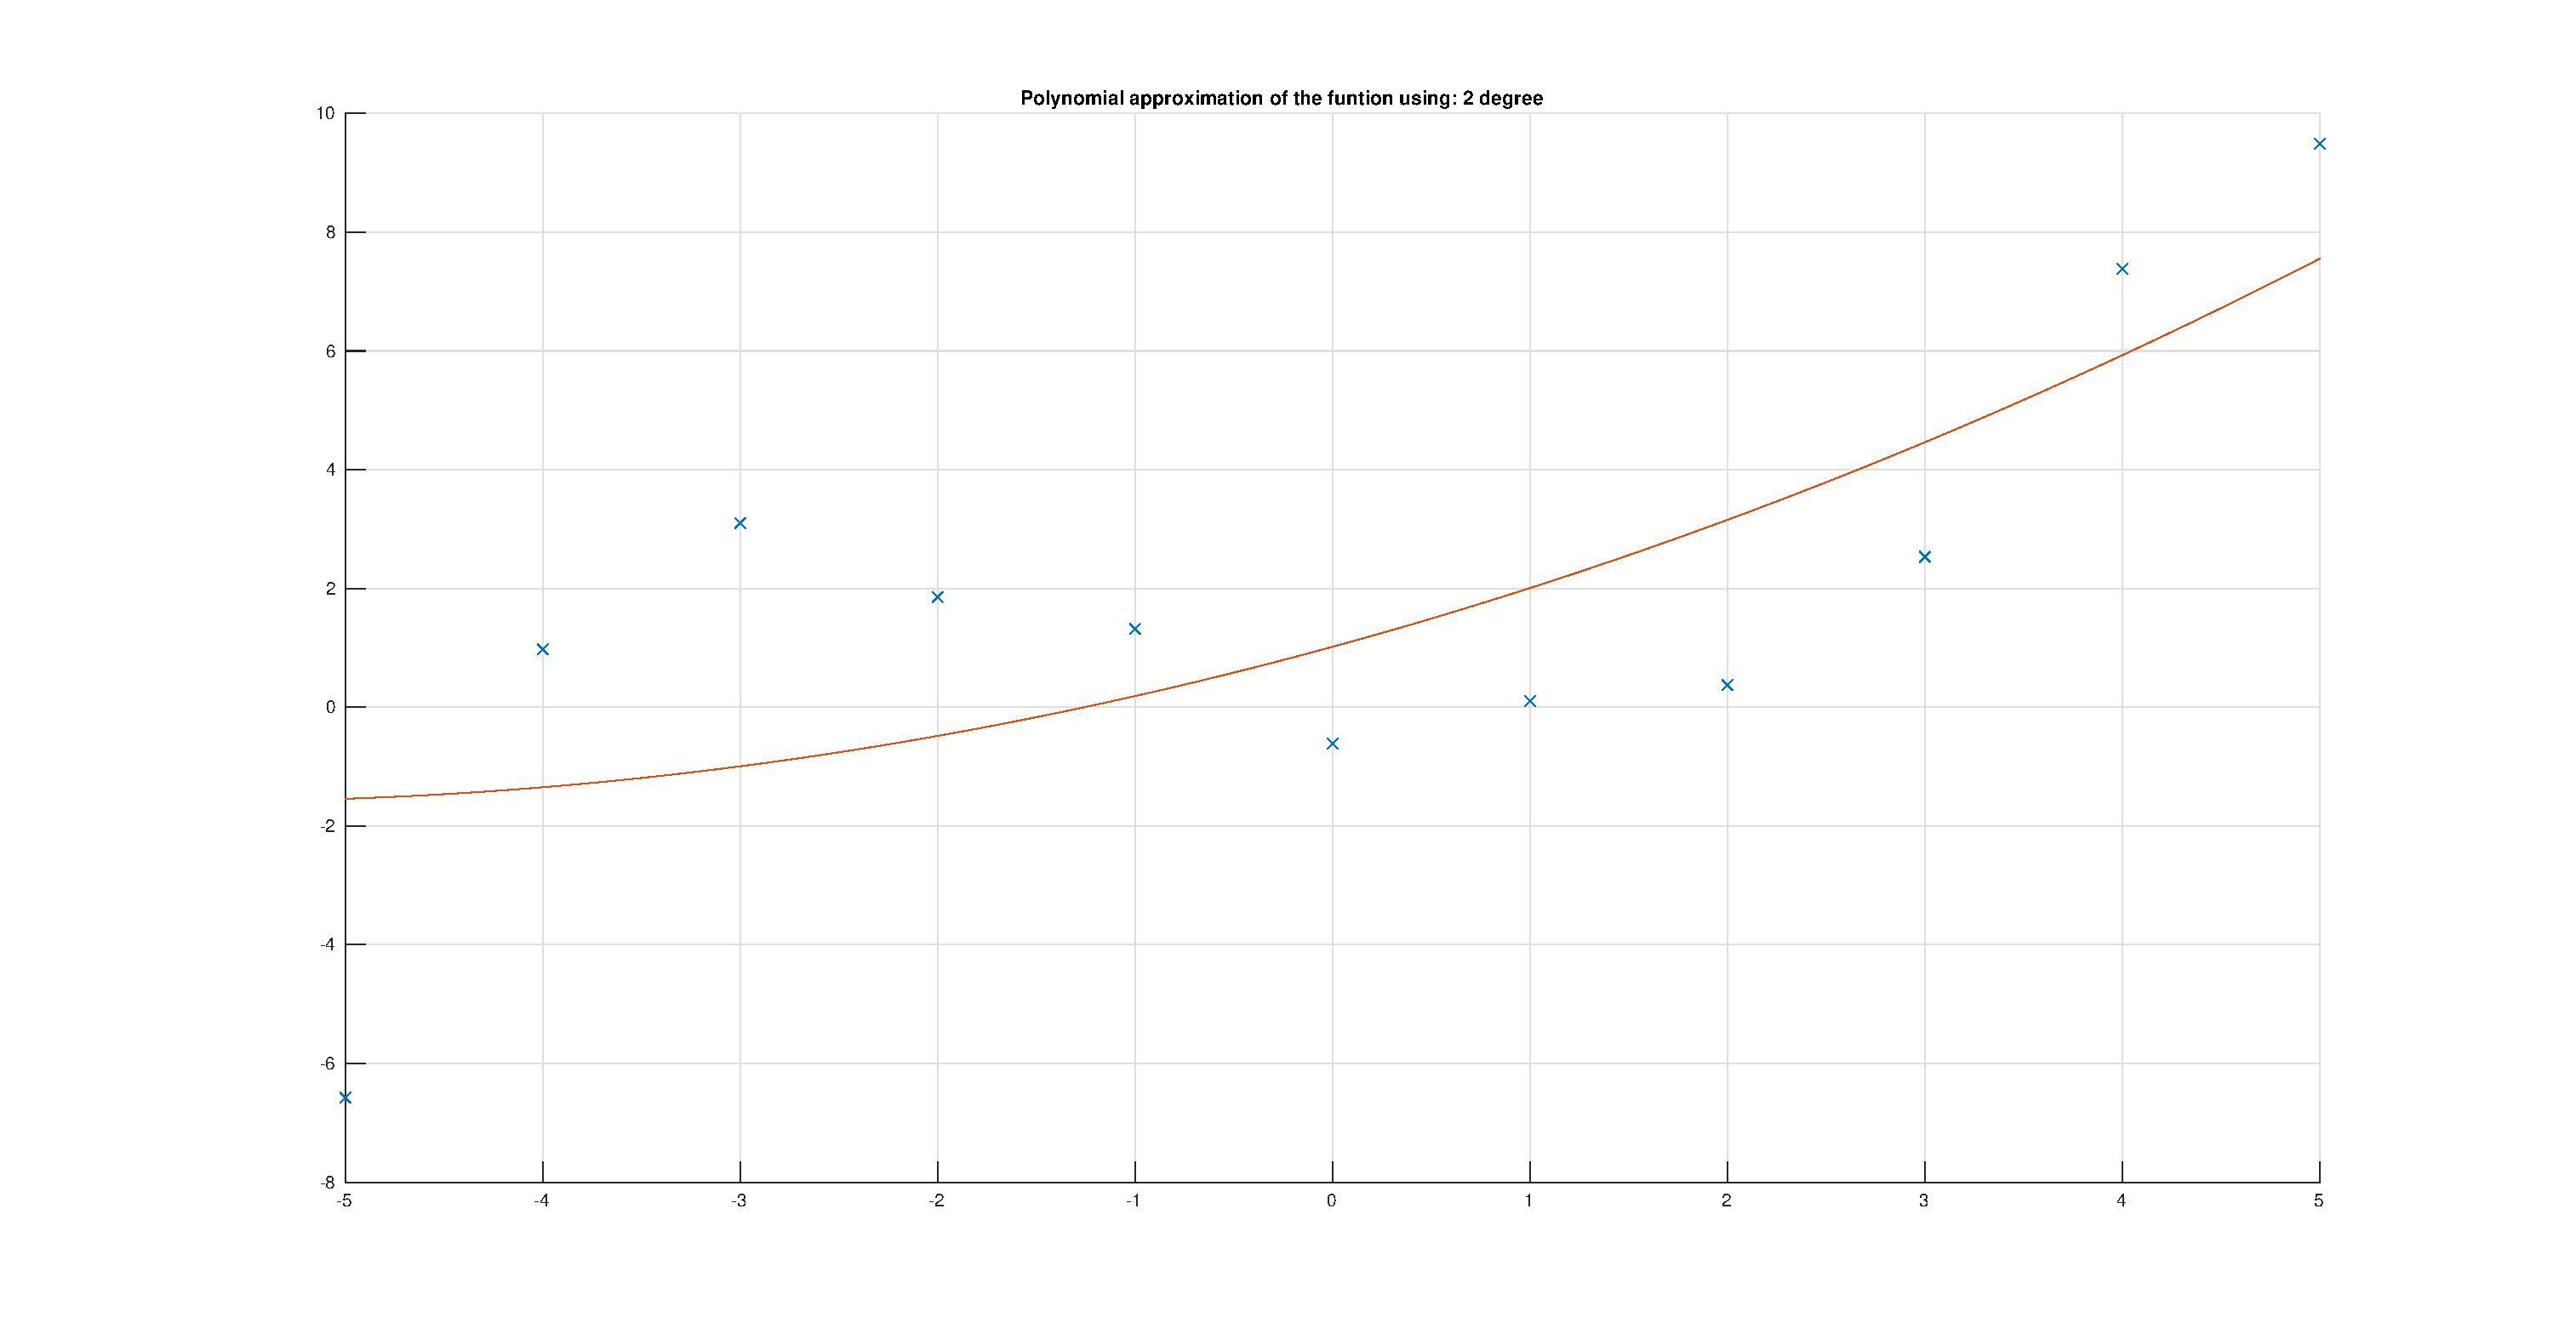
\includegraphics[scale=0.25]{12.eps}
\end{center}

\begin{center}
   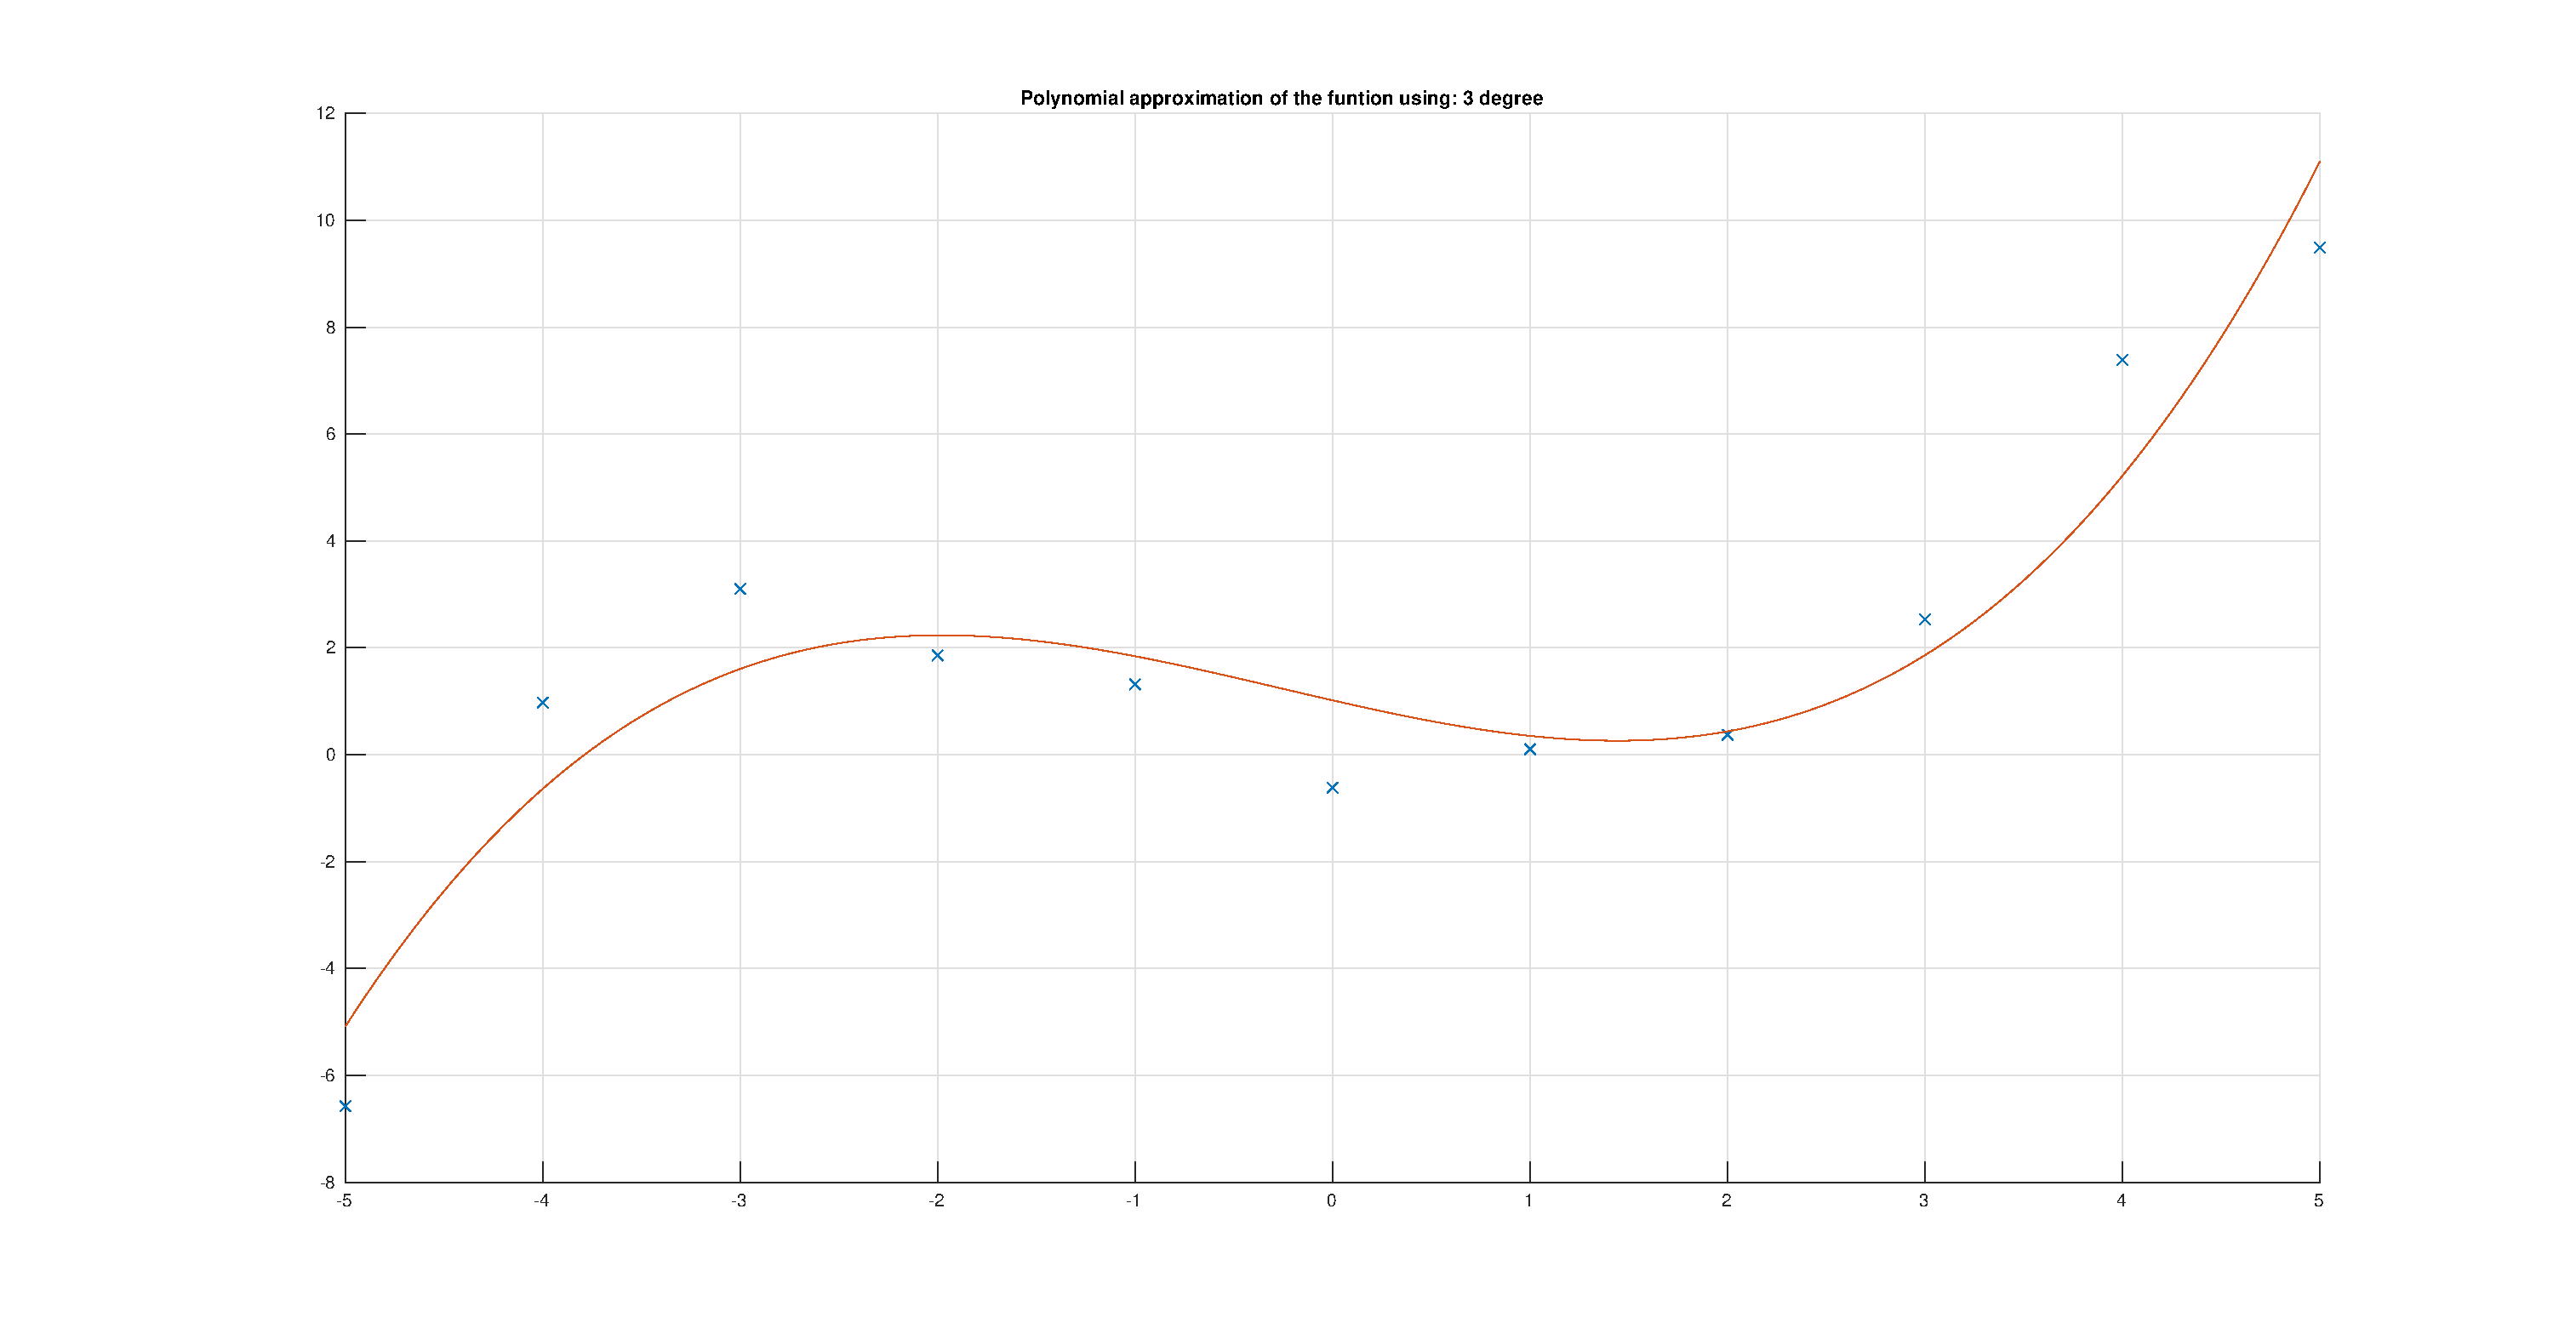
\includegraphics[scale=0.25]{13.eps}
\end{center}

\begin{center}
   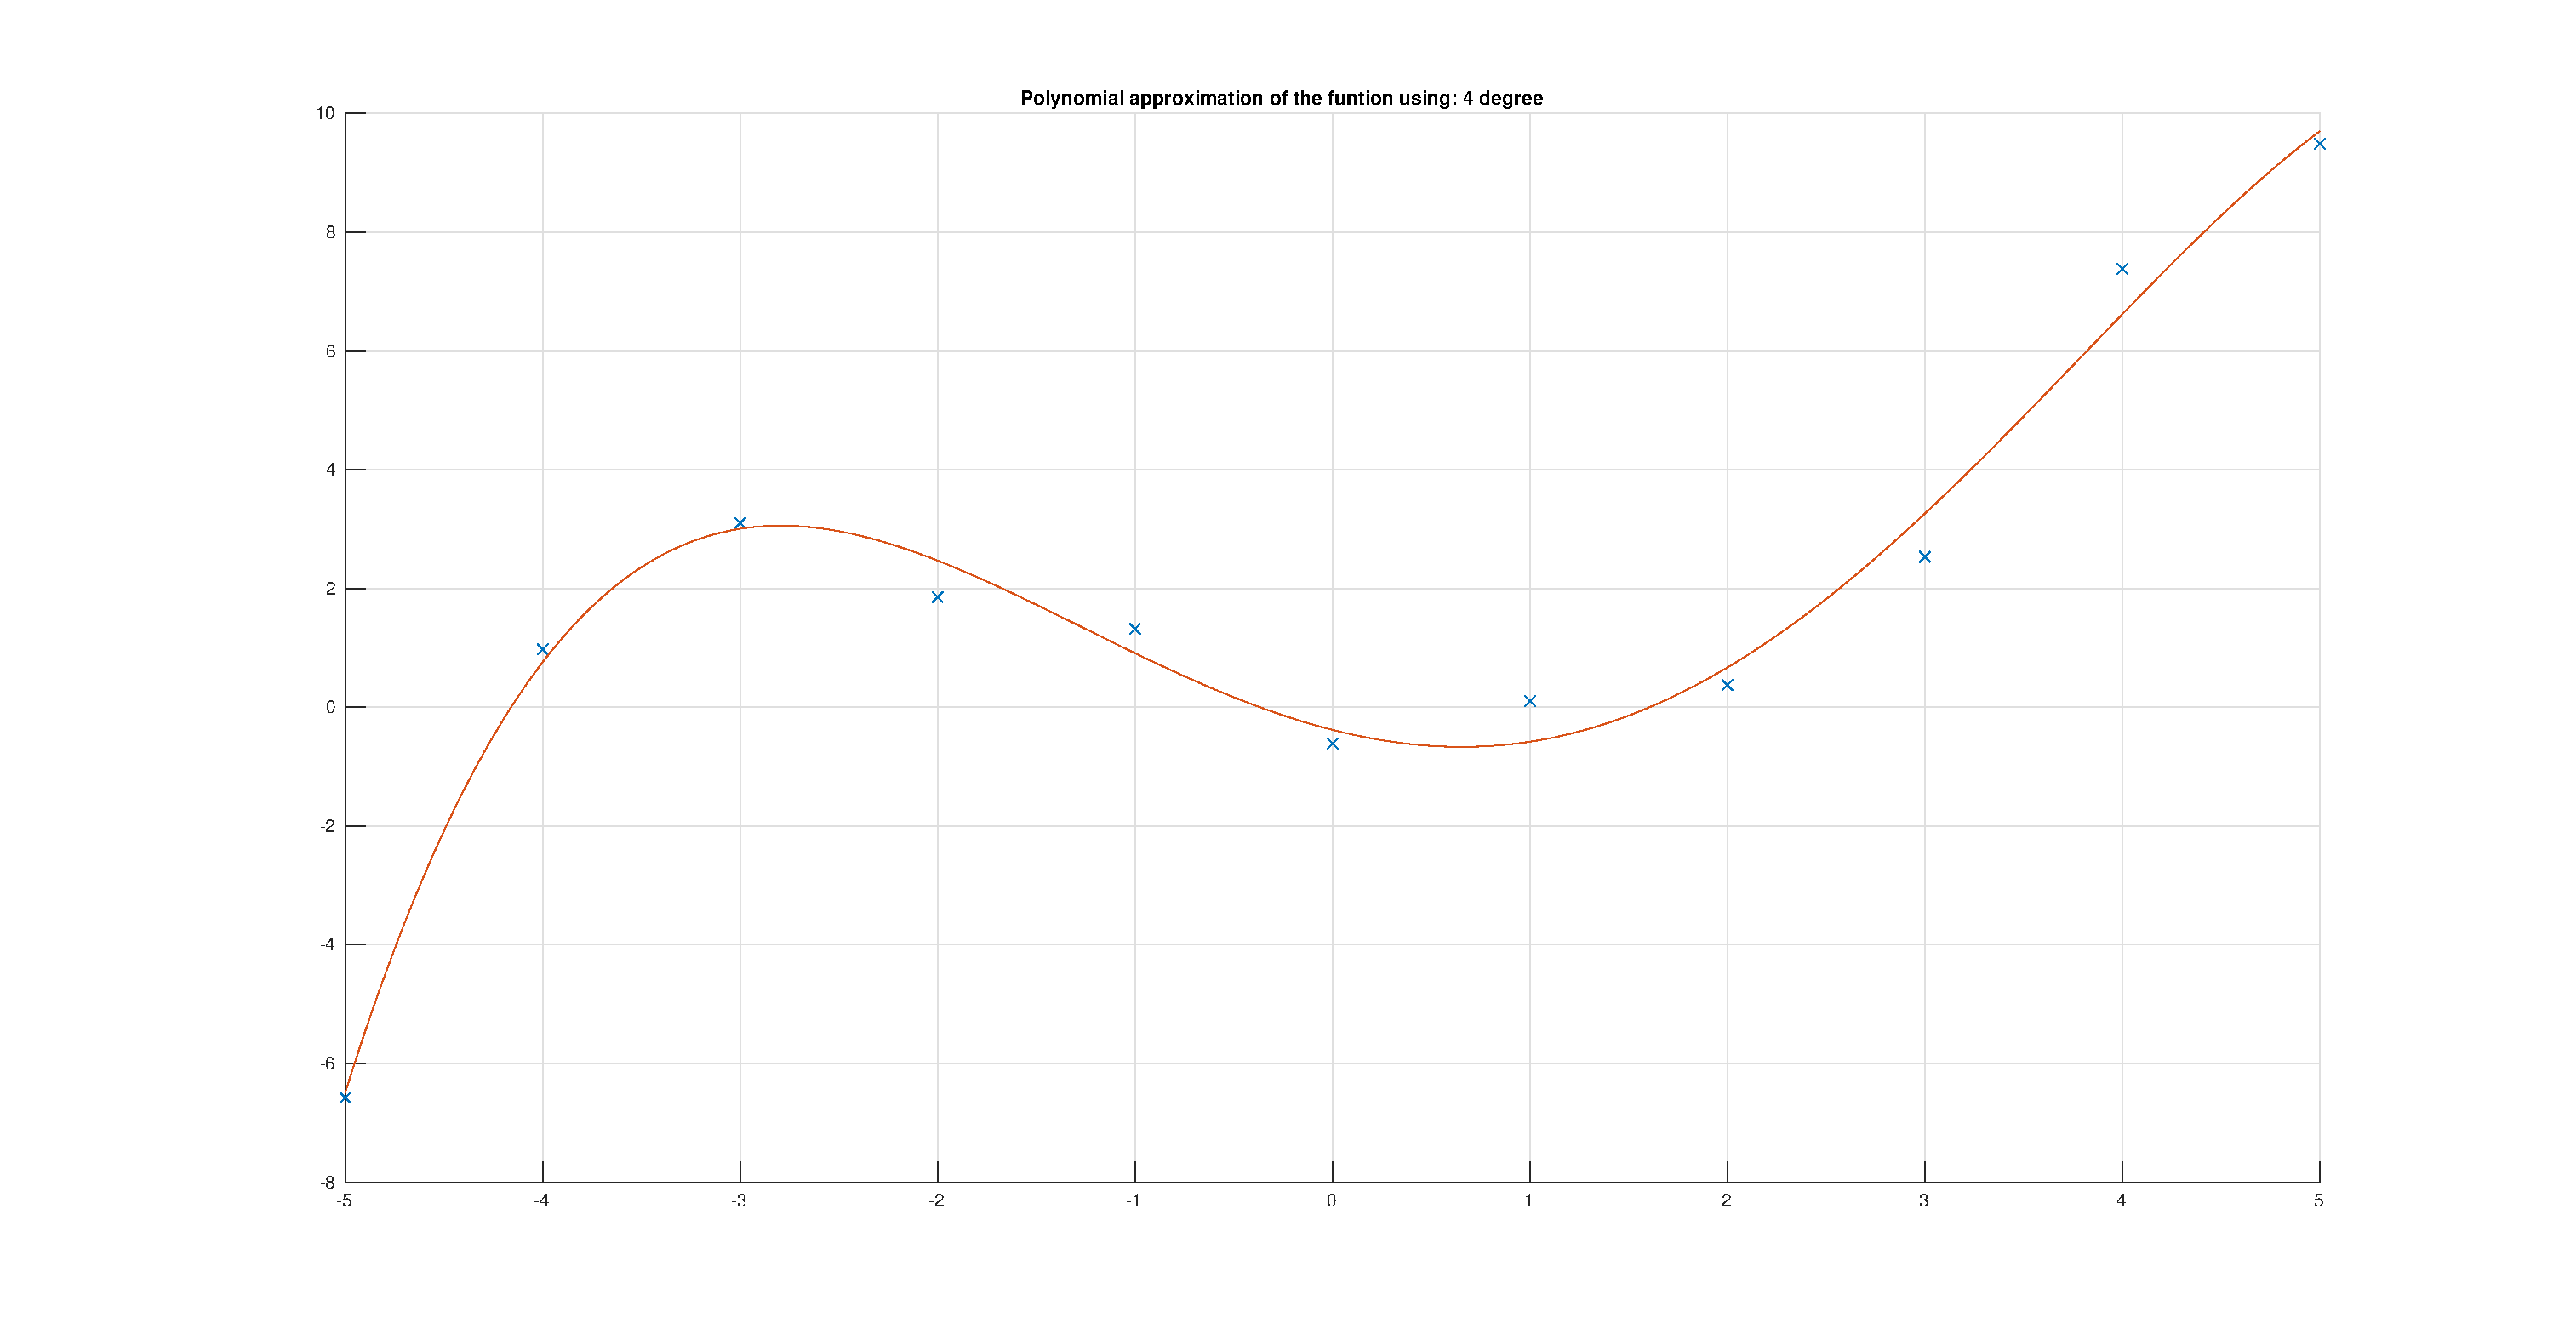
\includegraphics[scale=0.25]{14.eps}
\end{center}

\begin{center}
   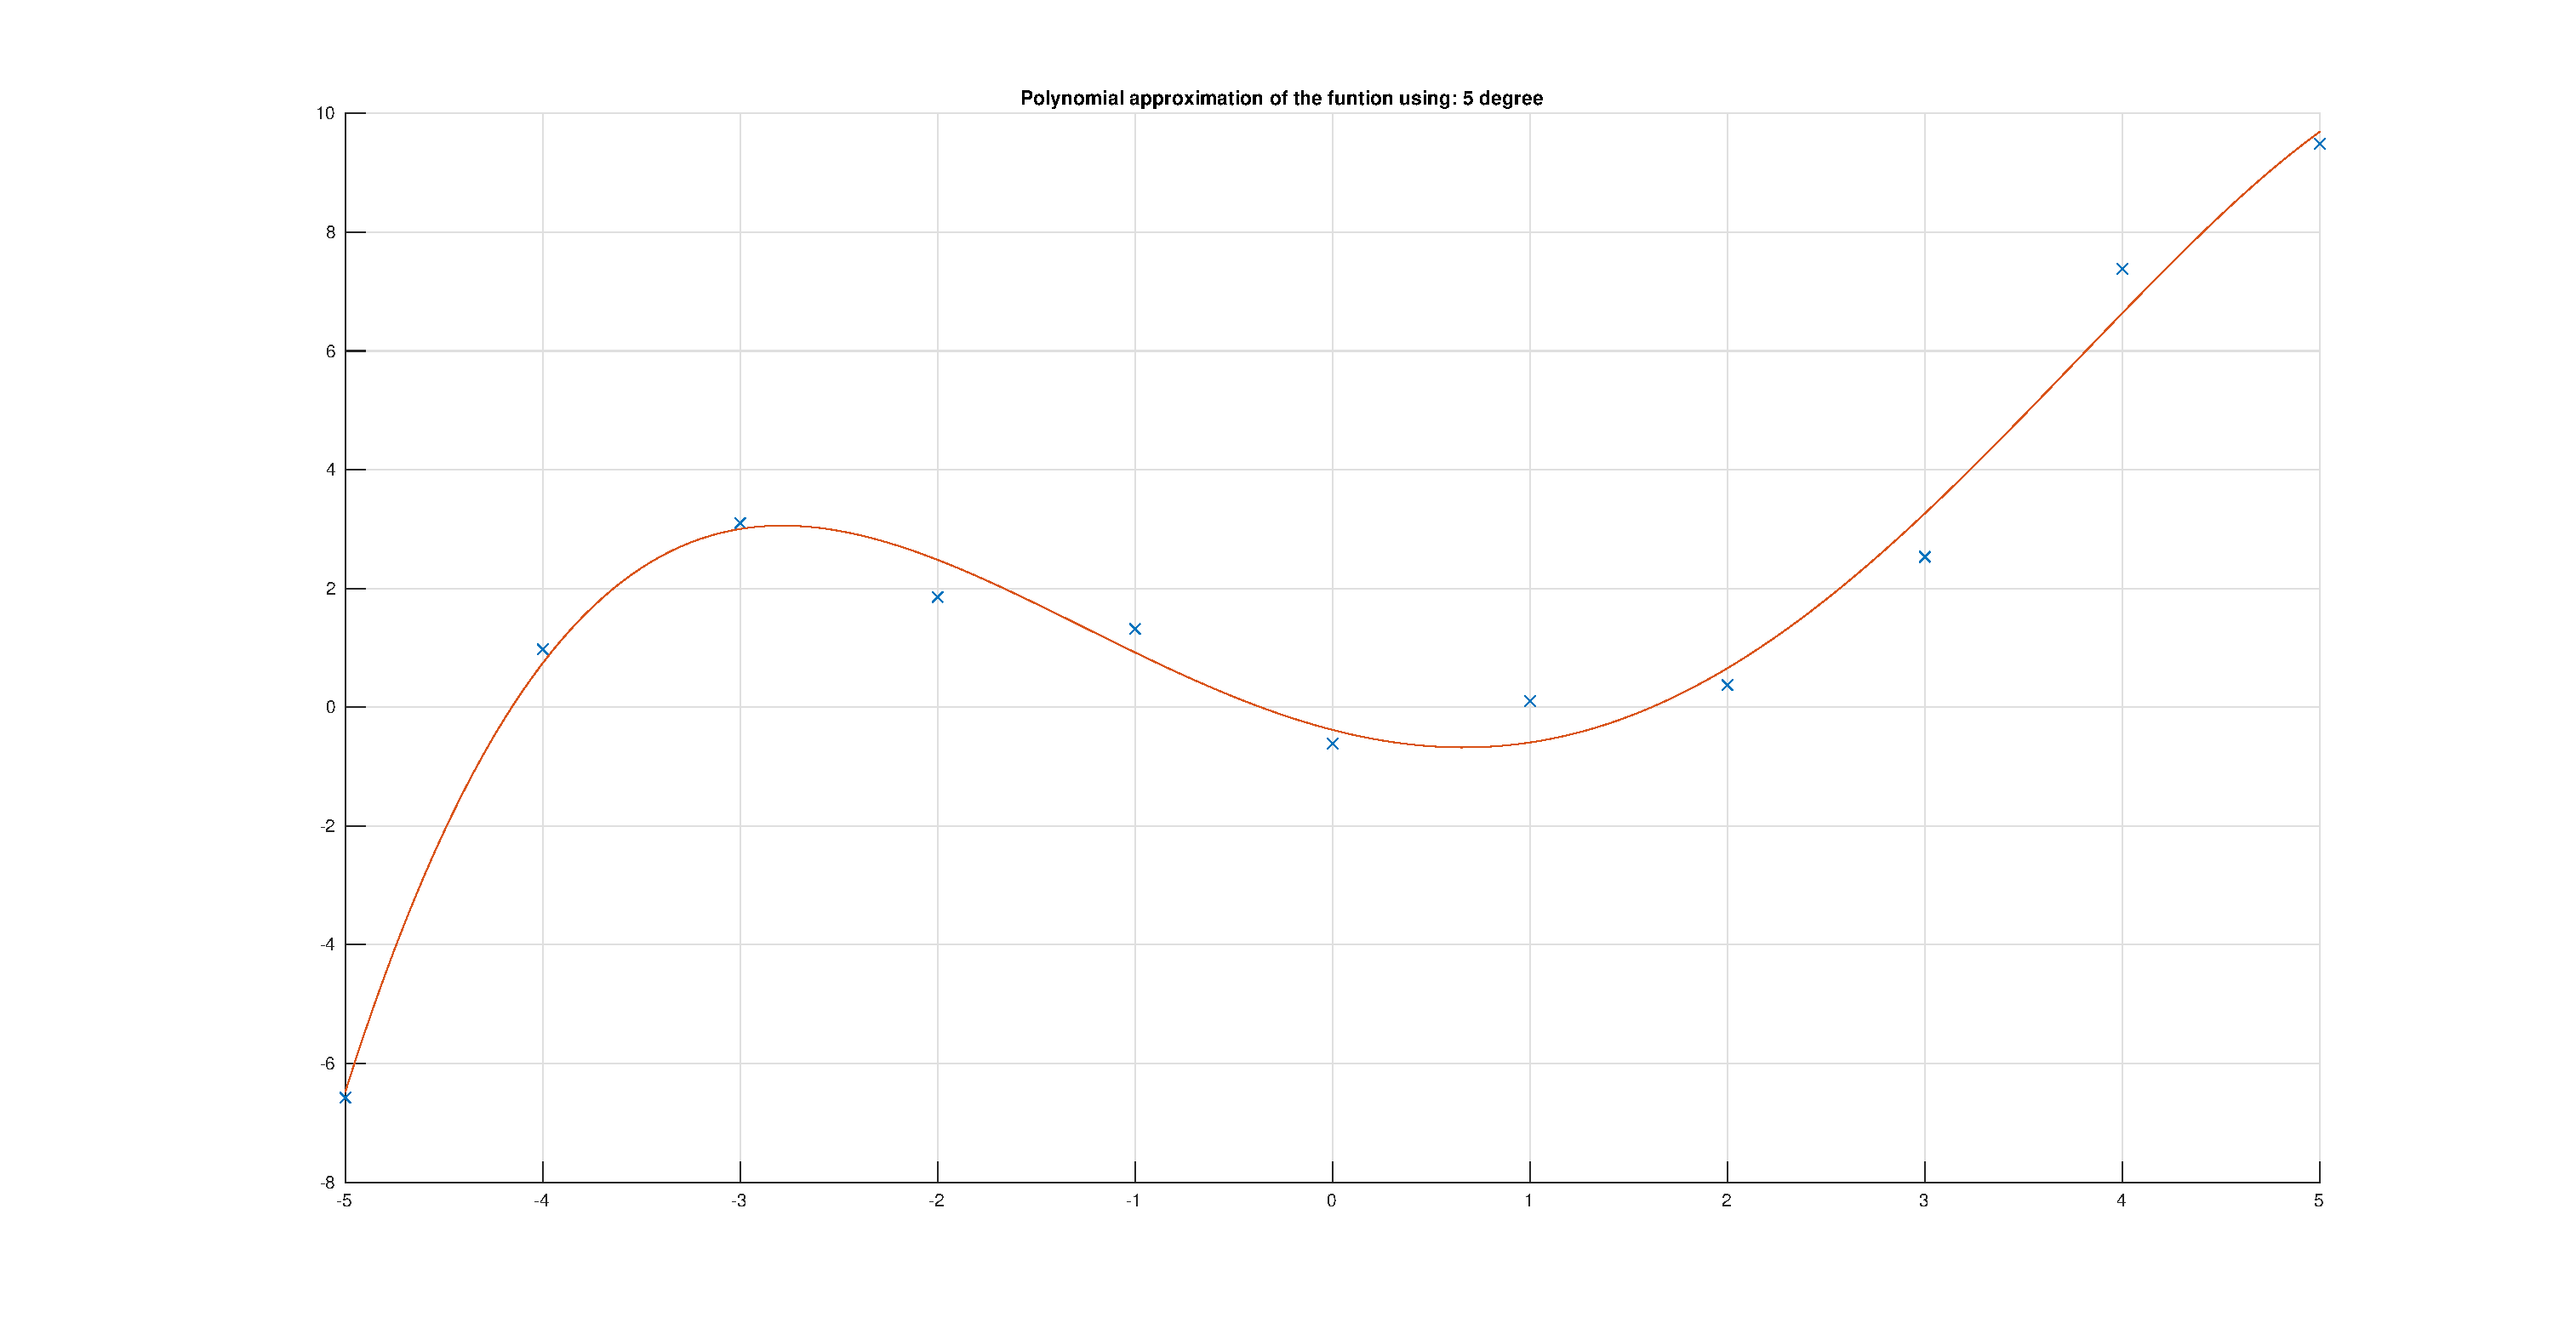
\includegraphics[scale=0.25]{15.eps}
\end{center}

\begin{center}
   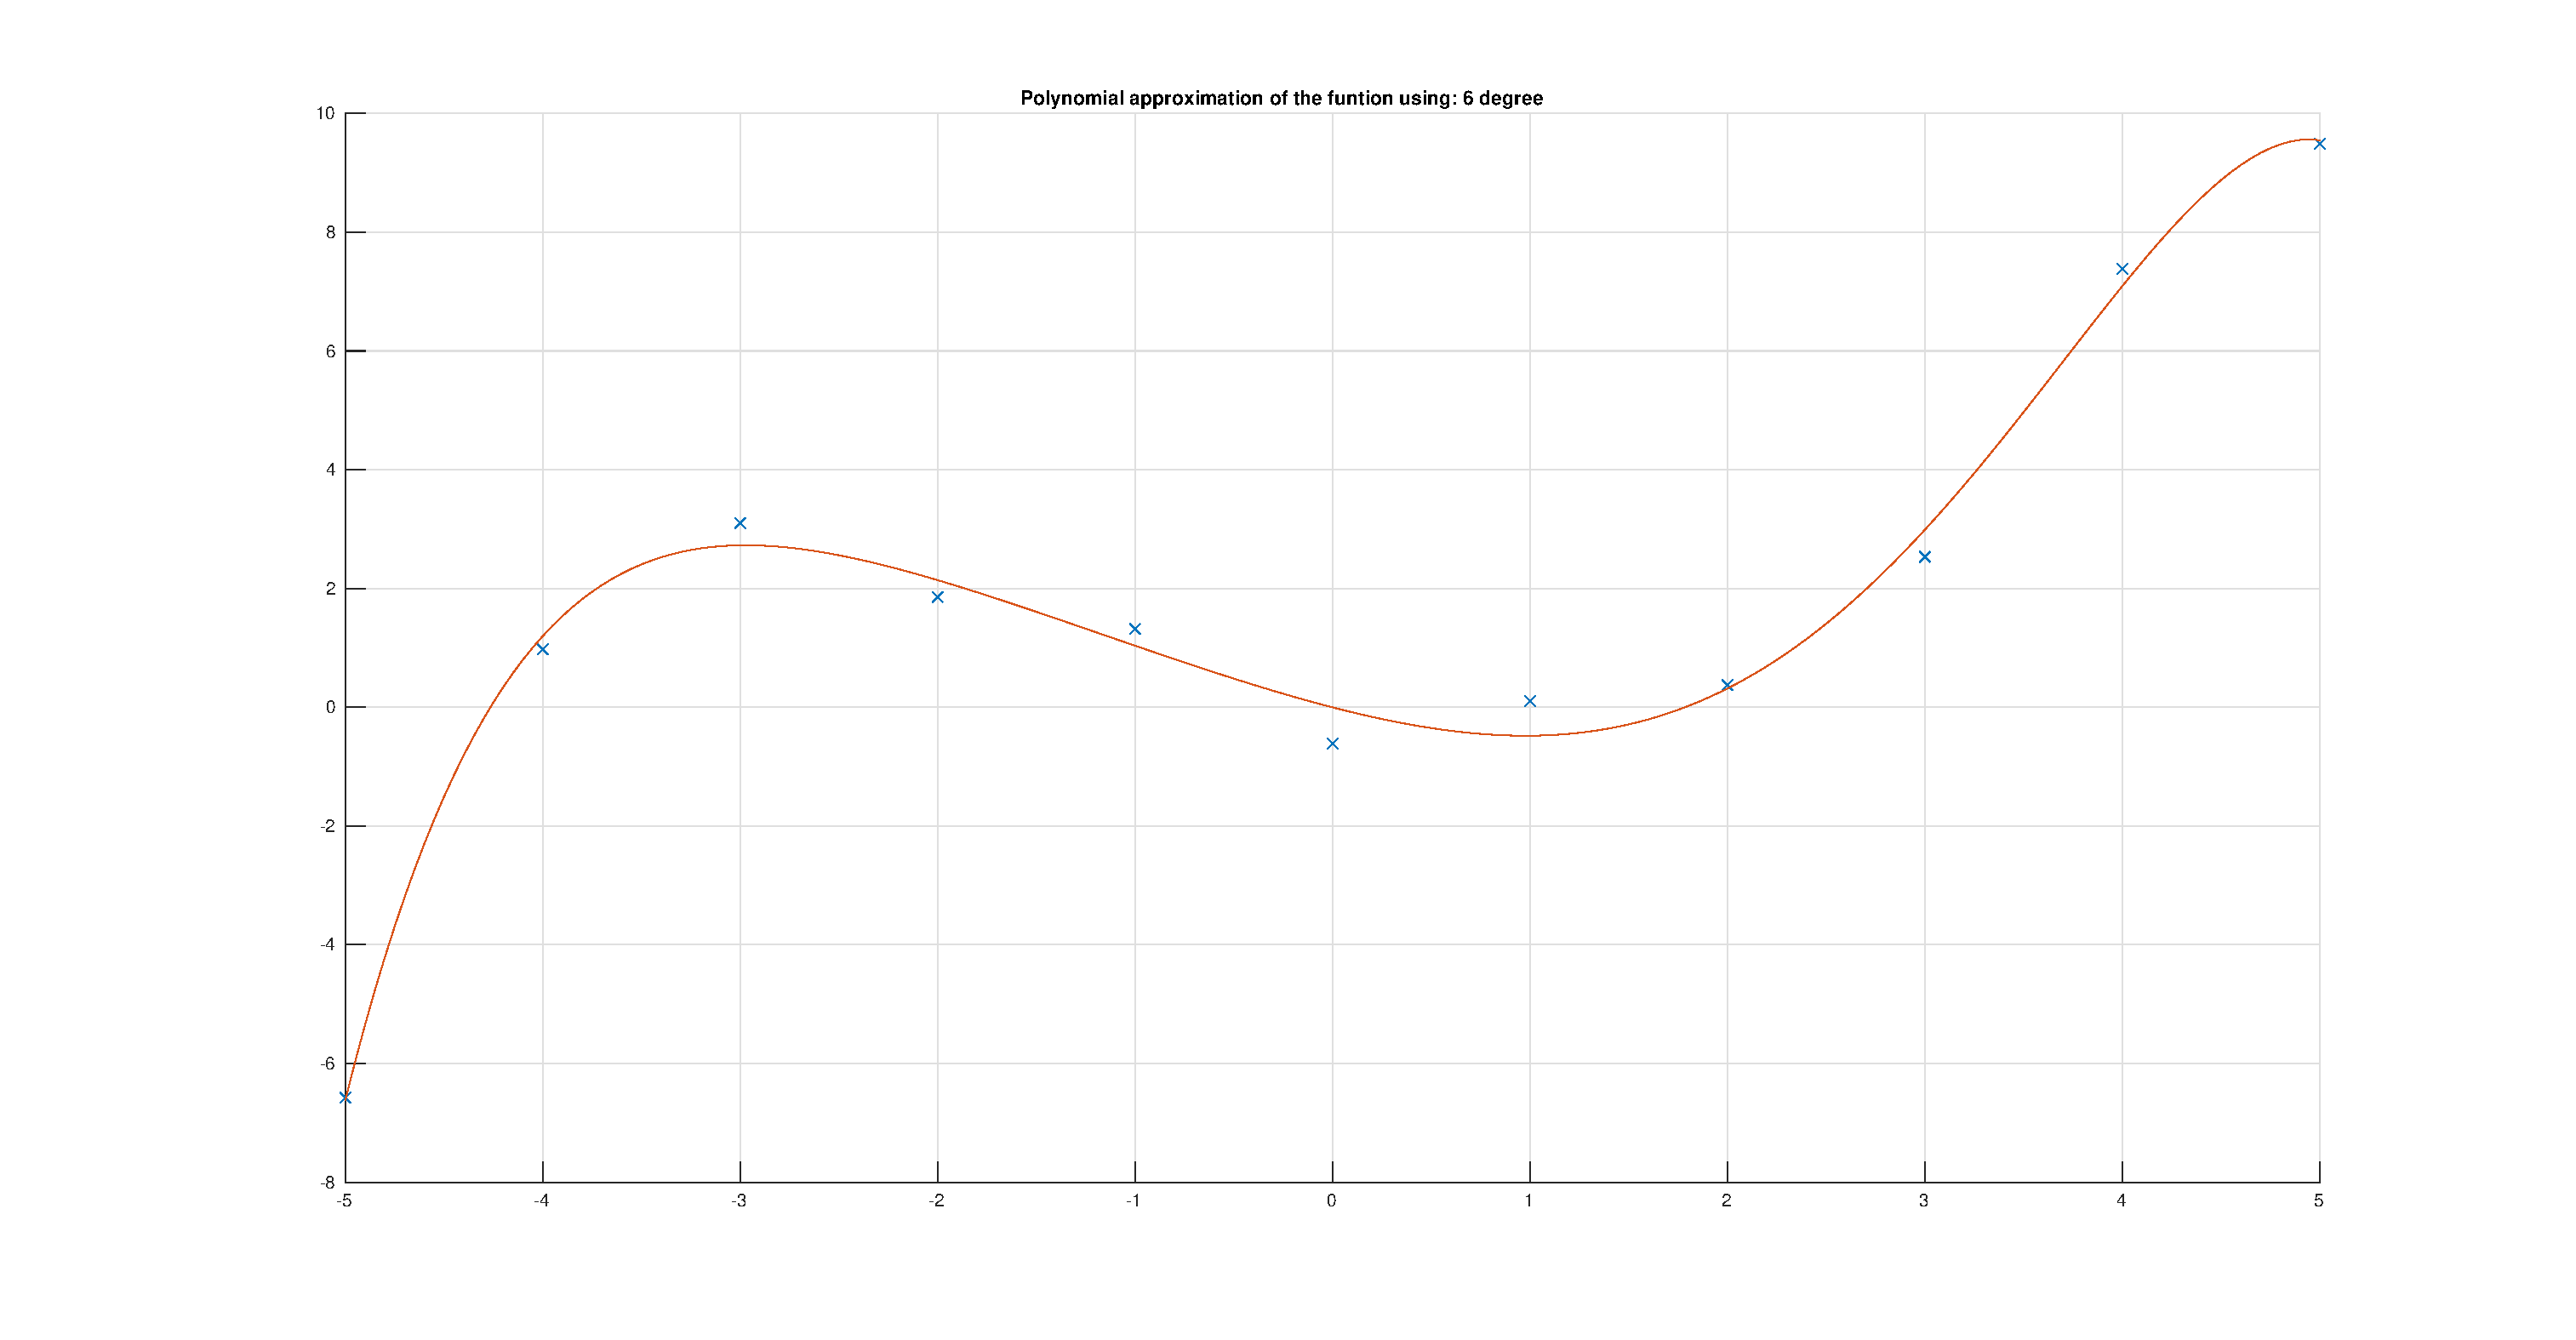
\includegraphics[scale=0.25]{16.eps}
\end{center}

\begin{center}
   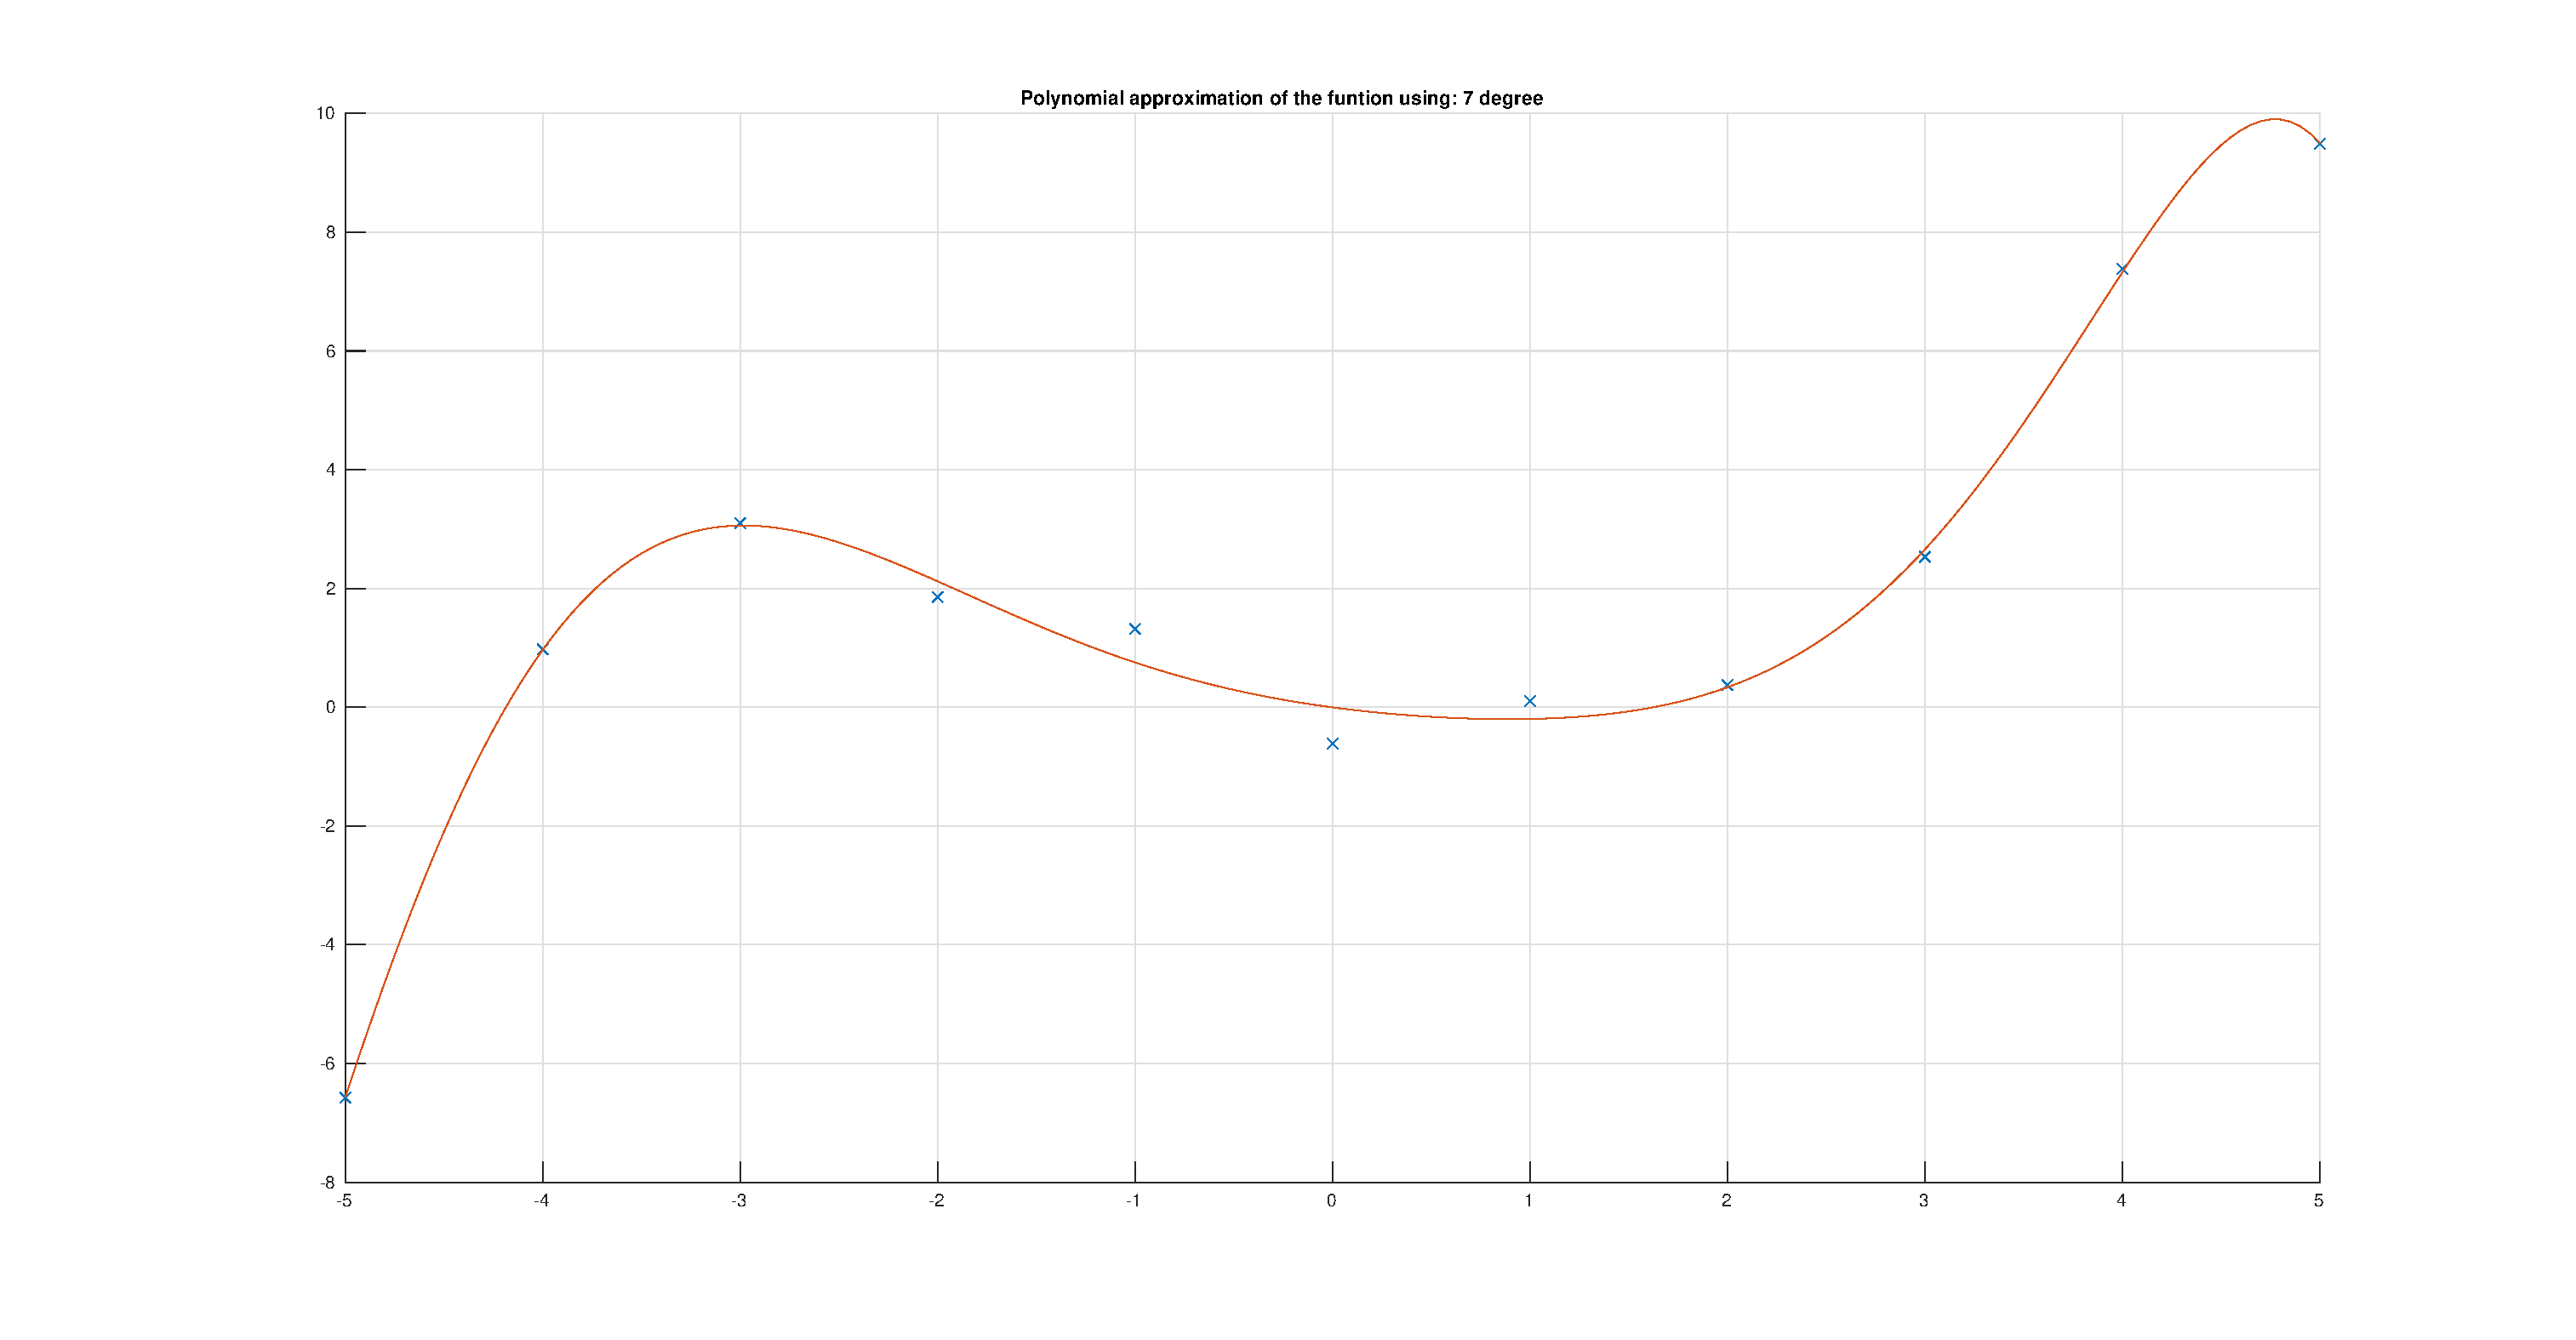
\includegraphics[scale=0.25]{17.eps}
\end{center}

\begin{center}
   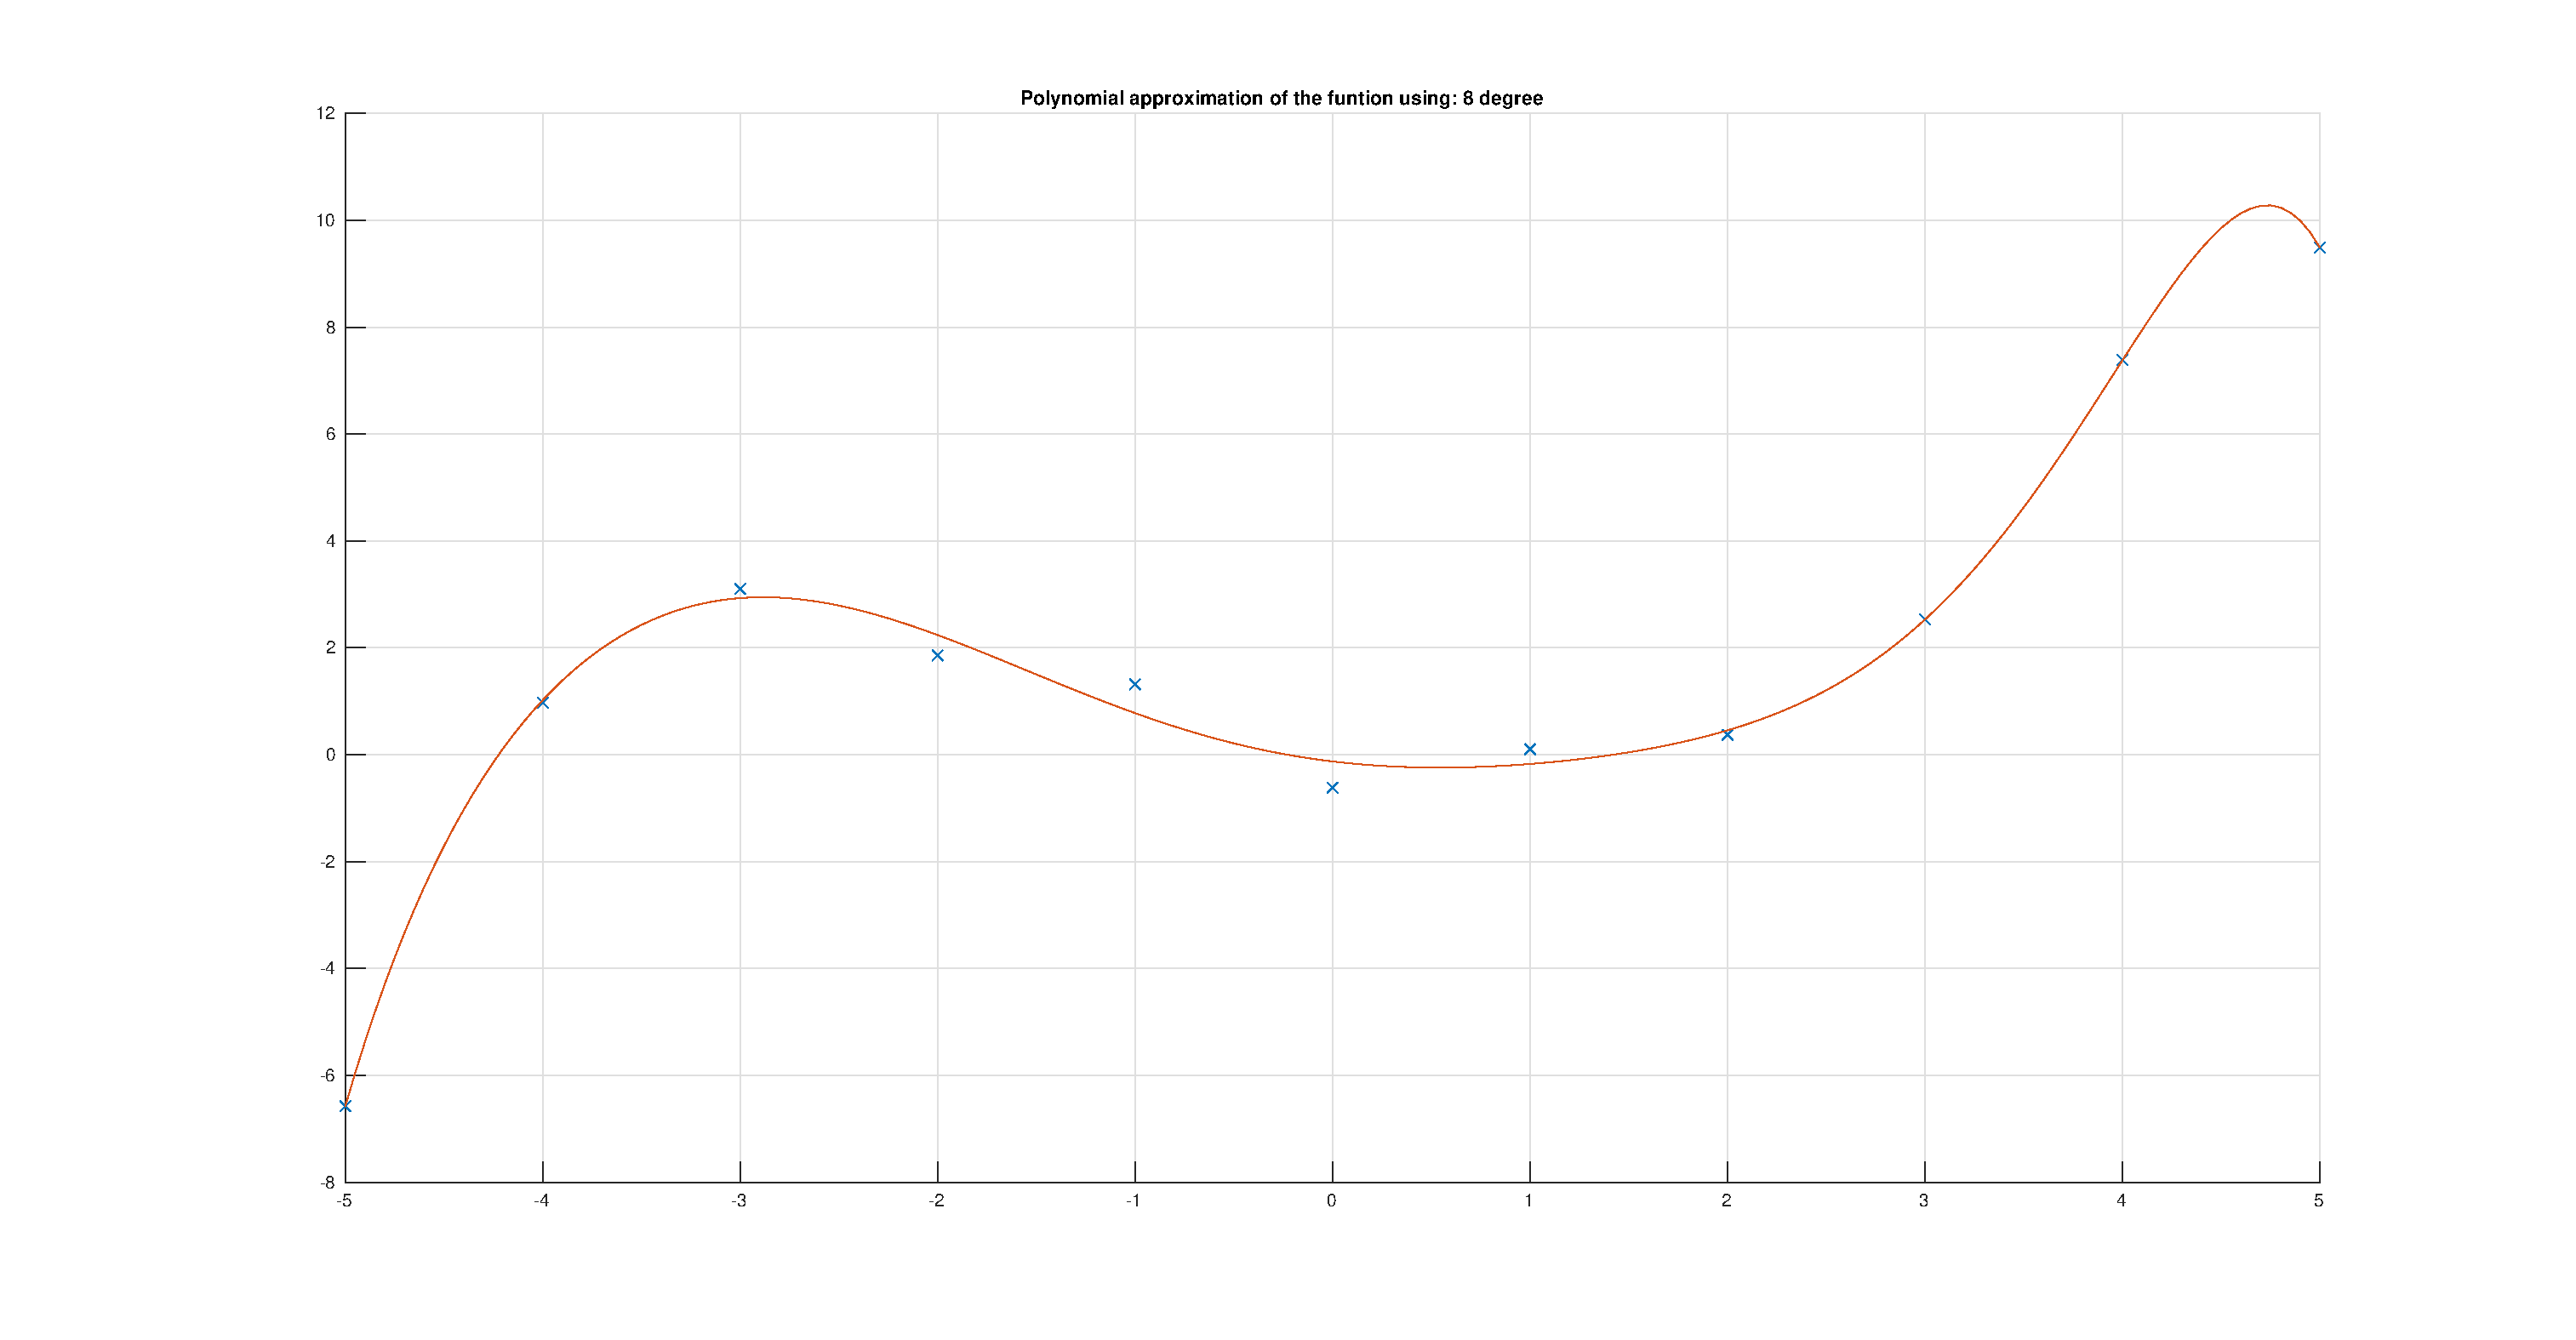
\includegraphics[scale=0.25]{18.eps}
\end{center}

\begin{center}
   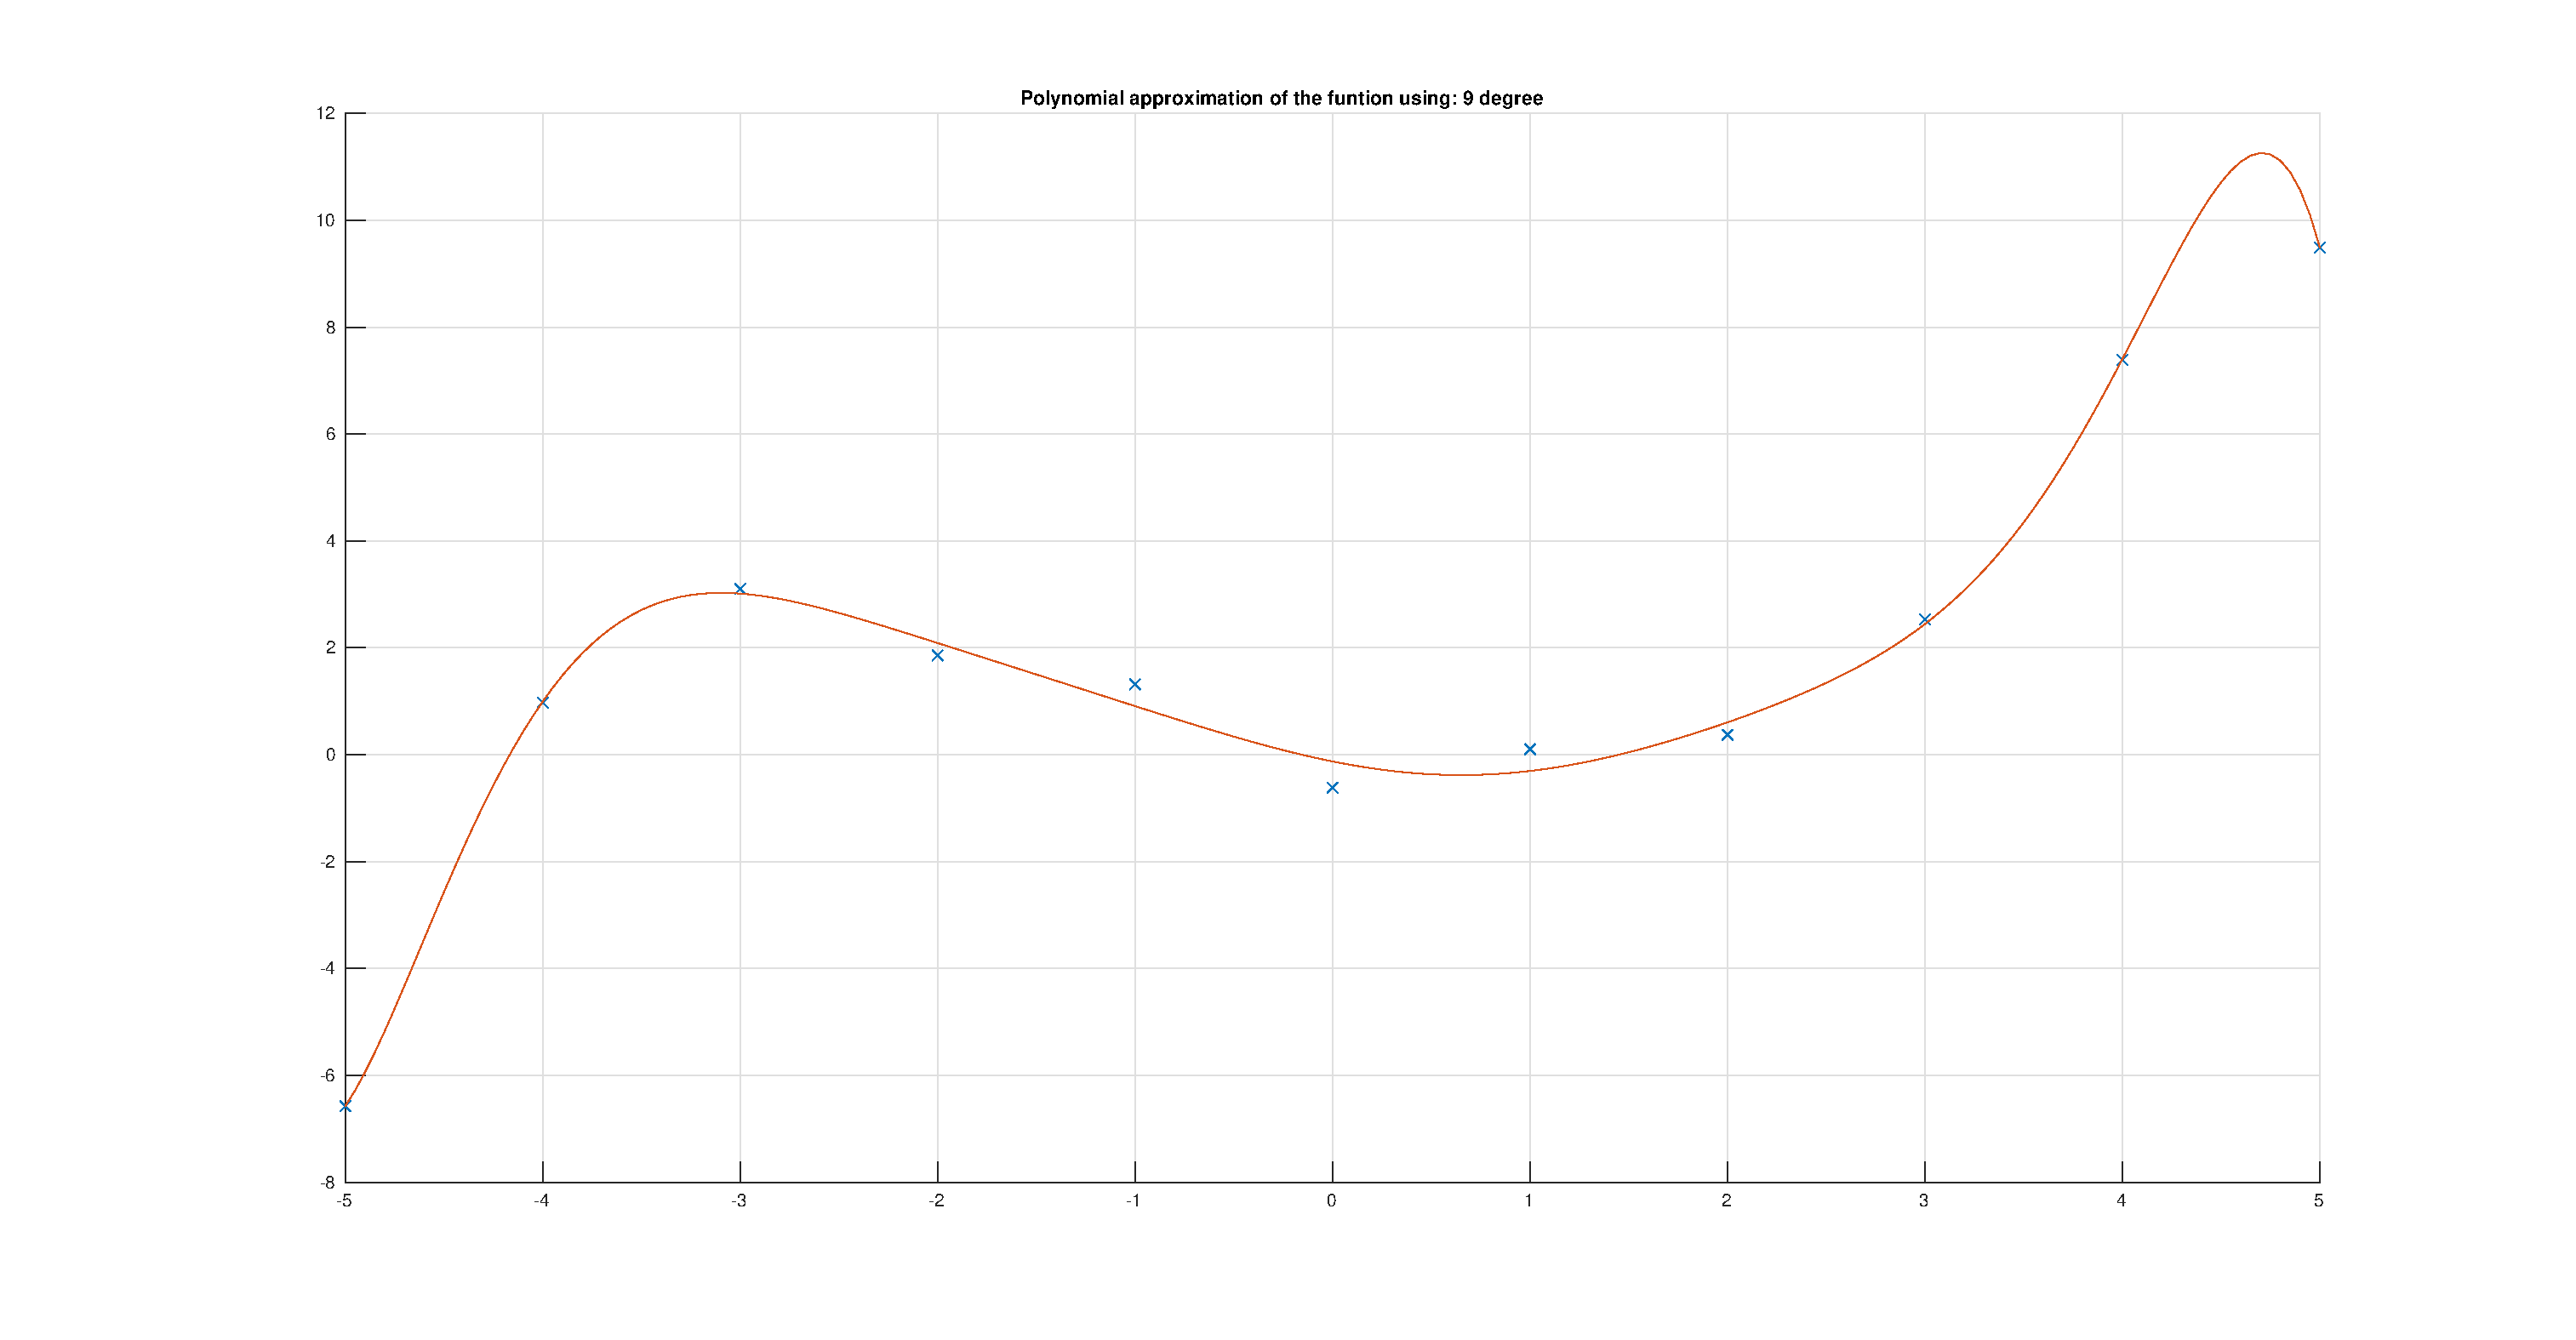
\includegraphics[scale=0.25]{19.eps}
\end{center}

\begin{center}
   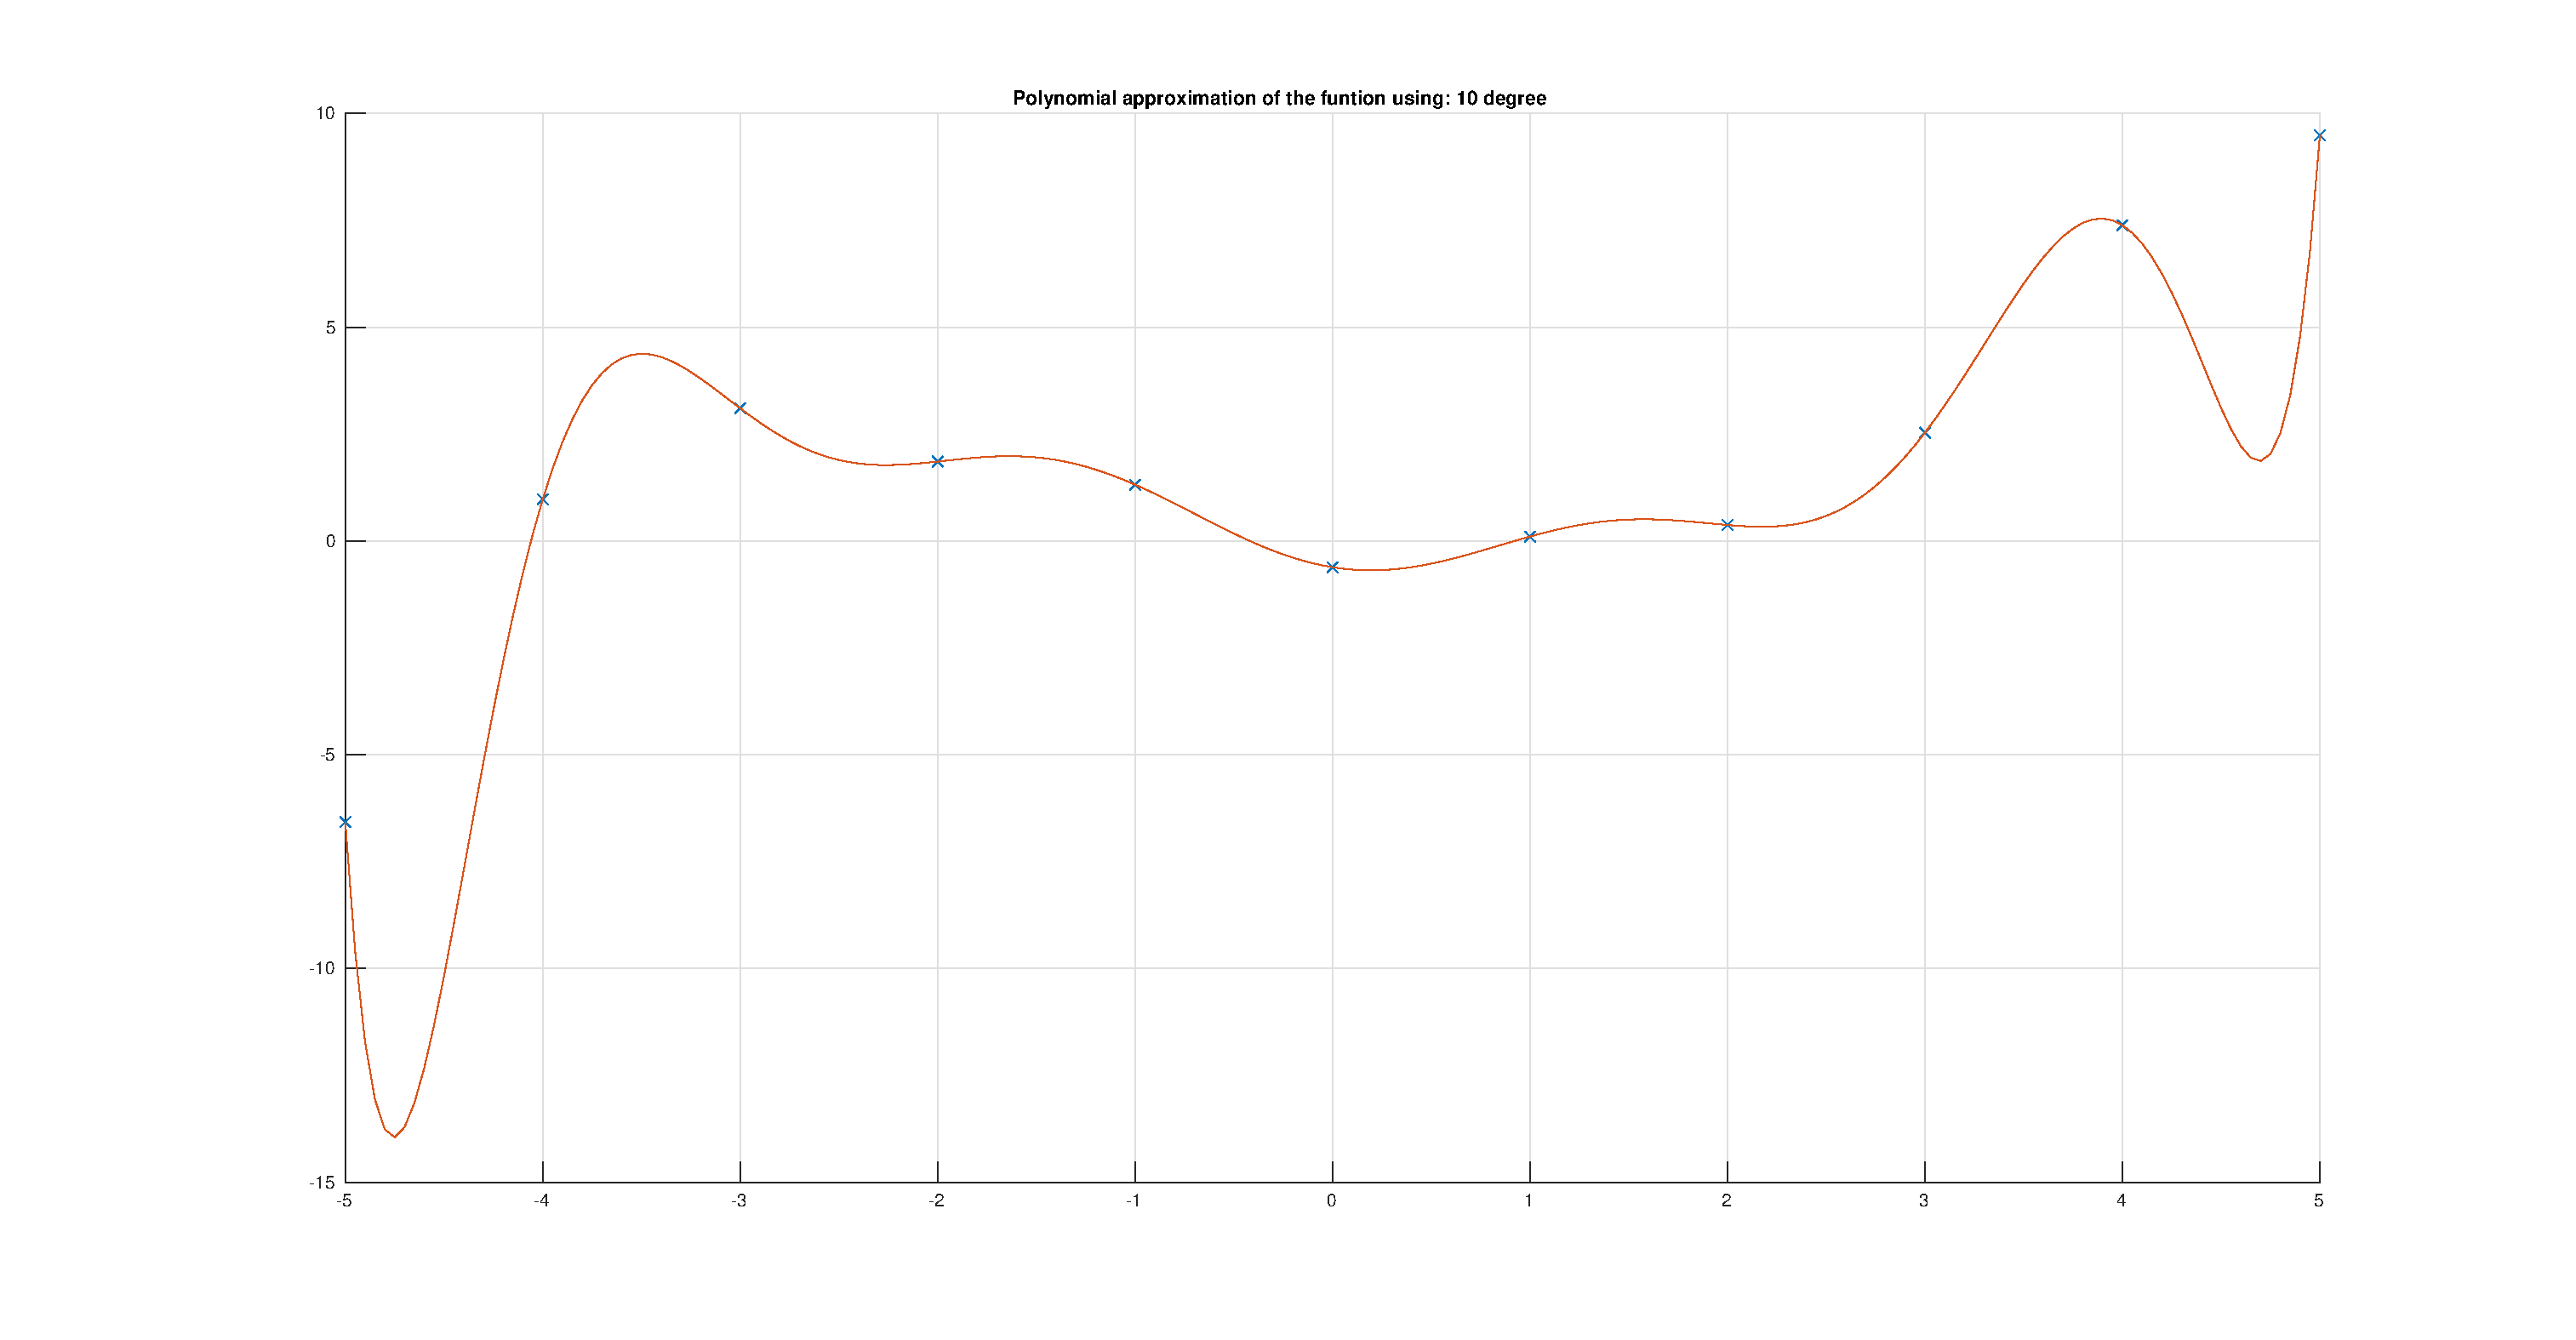
\includegraphics[scale=0.25]{110.eps}
\end{center}

\begin{center}
  \begin{tabular}{| c | c | c |}
\hline

Degree & Error & Condition number of Gram's Matrix \\
\hline
0& 13.2040& 1\\
\hline
1& 9.1281& 10\\
\hline
2& 8.8257&   408.7796\\
\hline
3& 4.2365& 8.5584e+03\\
\hline
4& 1.5418&  3.1798e+05\\
\hline
5& 1.5413& 7.4675e+06\\
\hline
6& 1.1689& 2.8316e+08\\
\hline
7& 0.9345& 7.6462e+09\\
\hline
8& 0.8883& 3.3055e+11\\
\hline
9& 0.8334& 1.5167e+13\\
\hline
10& 6.3645e-13& 9.2930e+14\\
\hline
  \end{tabular}
\end{center}







\chapter{Determine trajectory of the motion}


\section{a) Runge-Kutta method of $4^{th}$ order and Adams PC}
\subsection{Problem}
We are given following equations:
\[ \frac{dx_1}{dt} = x_2 + x_1(0.5 - x_1^2 - x_2^2) \]
\[ \frac{dx_2}{dt} = -x_1 + x_2(0.5 - x_1^2 - x_2^2) \]

And we have to determine the trajectory of the motion on interval $[0, 15]$ with following initial conditions:
$ x_1(0) = 8; x_2(0) = 9 $
In this section we will use Runge-Kutta method of $4^{th}$ order and Adams PC with different step-sizes until we find an optimal constant step size - when the decrease of the step size does not influence the solution significantly.

\subsection{Theoretical Introdution}
Determining the trajectory of the motion in this example can be mathematically described as solving a system of first order ordinary differential equations with given initical conditions. That is why we use Runge-Kutta method of order 4 which deals with exactly this kind of problem.
\subsubsection{Runge-Kutta method of order 4}
Any single step method are defined by the following formula, where h is a fixed step-size:
\[ y_{n+1} = y_n + \Phi_f(x_n, y_n, h) \]
where:
\[ x_n = x_0 + nh \]
\[ y(x_0) = y_0 = y_a \]
where $y_a$ is given.
Runge-Kutta method of order 4 - RK4 method looks like this:
\[ y_{n+1} = y_n + \frac{1}{6}(k_1 + 2k_2+2k_3+k_4) \]
\[ k_1 = f(x_n, y_n) \]
\[ k_3 = f(x_n + \frac{1}{2}h, y_n + \frac{1}{2}hk_1) \]
\[ k_2 = f(x_n + \frac{1}{2}h, y_n + \frac{1}{2}hk_2) \]
\[ k_4 = f(x_n + h, y_n + hk_3) \]


\subsection{Adams PC method}
Adams method with $P_kEC_kE$ algorithm has the following form: \\
P: \[  y_n^{[0]} = y_{n-1} + h\sum_{j=1}^k \beta_jf_{n-j} \]
E: \[  f_n^{[0]} = f(x_n, y_n^{[0]}) \]
C: \[  y_n = y_{n-1} + h \sum_{j=1}^k \beta_j^* f_{n-j} + h \beta_0^* f_n^{[0]}\]
E: \[  f_n = f(x_n, y_n) \]

When compared to explicit and implicit adams method PC metho has smaller absolute stability intervals than implicit method, while having significant advantage in calculations cost.



\section{b) Runge-Kutta method of $4^{th}$ order with variable step size automatically adjusted}
\subsection{Problem}
We are given following equations:
\[ \frac{dx_1}{dt} = x_2 + x_1(0.5 - x_1^2 - x_2^2) \]
\[ \frac{dx_2}{dt} = -x_1 + x_2(0.5 - x_1^2 - x_2^2) \]
And we have to determine the trajectory of the motion on interval $[0, 15]$ with following initial conditions:
$ x_1(0) = 8; x_2(0) = 9 $
In this section we will use Runge-Kutta method of $4^{th}$ order with step size automatically adjusted by the algorithm, with error estimation made according to the step-doubling rule.
\subsection{Theoretical Introdution}
Since Runge-Kutta method was explained in previous task I will focus on step-doubling rule.
Everytime we increase step size we receive less accurate results at the benefit of less calculations cost, this means that we need to have reasonable approach to setting step size to maximise accuracy and minimize calculations cost. We will use step-doubling rule in this example.

\subsubsection{Error estimation using step doubling-approach}
For every step of size $h$ we perform two additional steps of size $\frac{h}{2}$. We denote: \\
$y_n^{1}$ as a new point obtained using the original step-size $h$ \\
$y_n^{2}$ as a new point obtained using steps of the size $\frac{h}{2}$ \\
$r^{(1)}$ - approximation error affter the single step $h$ \\
$r^{(2)}$ - summed approximation errors after the two smaller steps of length $\frac{h}{2}$ each. \\
We have: \\
\newpage
After a single step:
\[ y(x_n + h) = y_n^{(1)} + \frac{r_n^{p+1}(0)}{(p+1)!}h^{p+1} + O(h^{p+2}) \]
After a double step:
\[  y(x_n+h) \simeq y_n^{(2)} + 2\frac{r_n^{p+1}(0)}{(p+1)!}(\frac{h}{2})^{p+1} + O(h^{p+2}) \]

We evaluate unknown coefficient from the first equation $ \frac{r_n^{p+1}(0)}{(p+1)!} $ and insert it into second one:
\[ y(x_n+h) = y_n^{(2)} + \frac{h^{p+1}}{2^p}\frac{(x_n+h) - y_n^{(1)}}{h^{p+1} + O(h^{p+2})} \]
We continue further and receive:
\[ y(x_n + h)(1-\frac{1}{2^p}) = y_n^{(2)}(1-\frac{1}{2^p}) + \frac{y_n^{2}}{2^p} - \frac{y_n^{(1)}}{2^p} + O(h^{p+2}) \]
We multiply by $\frac{2^p}{2^p - 1}$ and get:
\begin{equation}
y(x_n+h) = y_n^{(2)} + \frac{ y_n^{(2)} - y_n^{(1)} }{ 2^p - 1 } + O(h^{p+2})
\end{equation}
We also obtain for first equation in a similar way:
 \[ y(x_n+h) = y_n^{(1)} + 2^p\frac{y_n^{(2)} - y_n^{(1)}}{2^p - 1} + O(h^{p+2}) \]
Assuming we take the main part of the error we get error estimate:
\[ \delta_n(h) = \frac{2^p}{2^p-1}(y_n^{(2)} - y_n^{(1)}) \]
But from the equation (2.1) we can treat expression:
\[ \delta_n(2 \times \frac{h}{2}) = \frac{ y_n^{(2)} - y_n^{(1)}}{2^p - 1} \]
as en estimate of the error of two consecutive steps of size $\frac{h}{2}$
\subsubsection{Actual correction of the step size}
In general formula for main part of the approximation error where:
\\ $h$ - length of a step
\[ \gamma = \frac{r_n^{(p+1)}(0)}{(p+1)!} \]
Looks like this:
\[ \delta_n(h) = \gamma h^{p+1} \]
If we change step-size to $\alpha h$ then we get:
\[ \delta_n(\alpha h) = \gamma (\alpha h)^{p+1} \]
Then:
\[ \delta_n(\alpha h) = \alpha^{p+1} \delta_n (h) \]
We assume tolerance $\epsilon$:
\[ |\delta_n(\alpha h)| = \epsilon \]
We get:
\[ \alpha^{p+1}|\delta_n(h)| = \epsilon \]
Coefficient $\alpha$ for the step-size correction can be evaluated in such a way:
\[ \alpha = (\frac{\epsilon}{|\delta_n (h)|})^{\frac{1}{p+1}} \]

This method is also correct for RK4 method when $\delta_n(h) = \delta_n(2 \times \frac{h}{2}) $
We should also take into considertaion lack of accuracy we do so by using safety factor $s$:
\[ h_{n+1} = s \alpha h_n \]
where $ s < 1 $
For RK4 we use $ s \approx 0.9 $ \\
We define accuracy parameters in such a way:
\[ \epsilon = |y_n| \epsilon_r + \epsilon_a \]
where $\epsilon_r$ is relative tolerance and $\epsilon_a$ is absolute tolerance. \\
In case of set of more than on differential equations we must use worst case approach so the equations that need smallest step-size define step-size for all other equations.
\newpage
For RK methods we have following parameters:
\[ \delta_n(h)_i = \frac{(y_i)_n^{(2)} - (y_i)_n^{(1)}}{2^p - 1} \]
\[ \epsilon_i = |(y_i)_n^{(2)}| \epsilon_r + \epsilon_a \]
\[ \alpha = \min_{1 \leq i \leq m} (\frac{\epsilon_i}{|\delta_n(h)_i}|)^{\frac{1}{p+1}} \]

\section{Results}

\begin{center}
   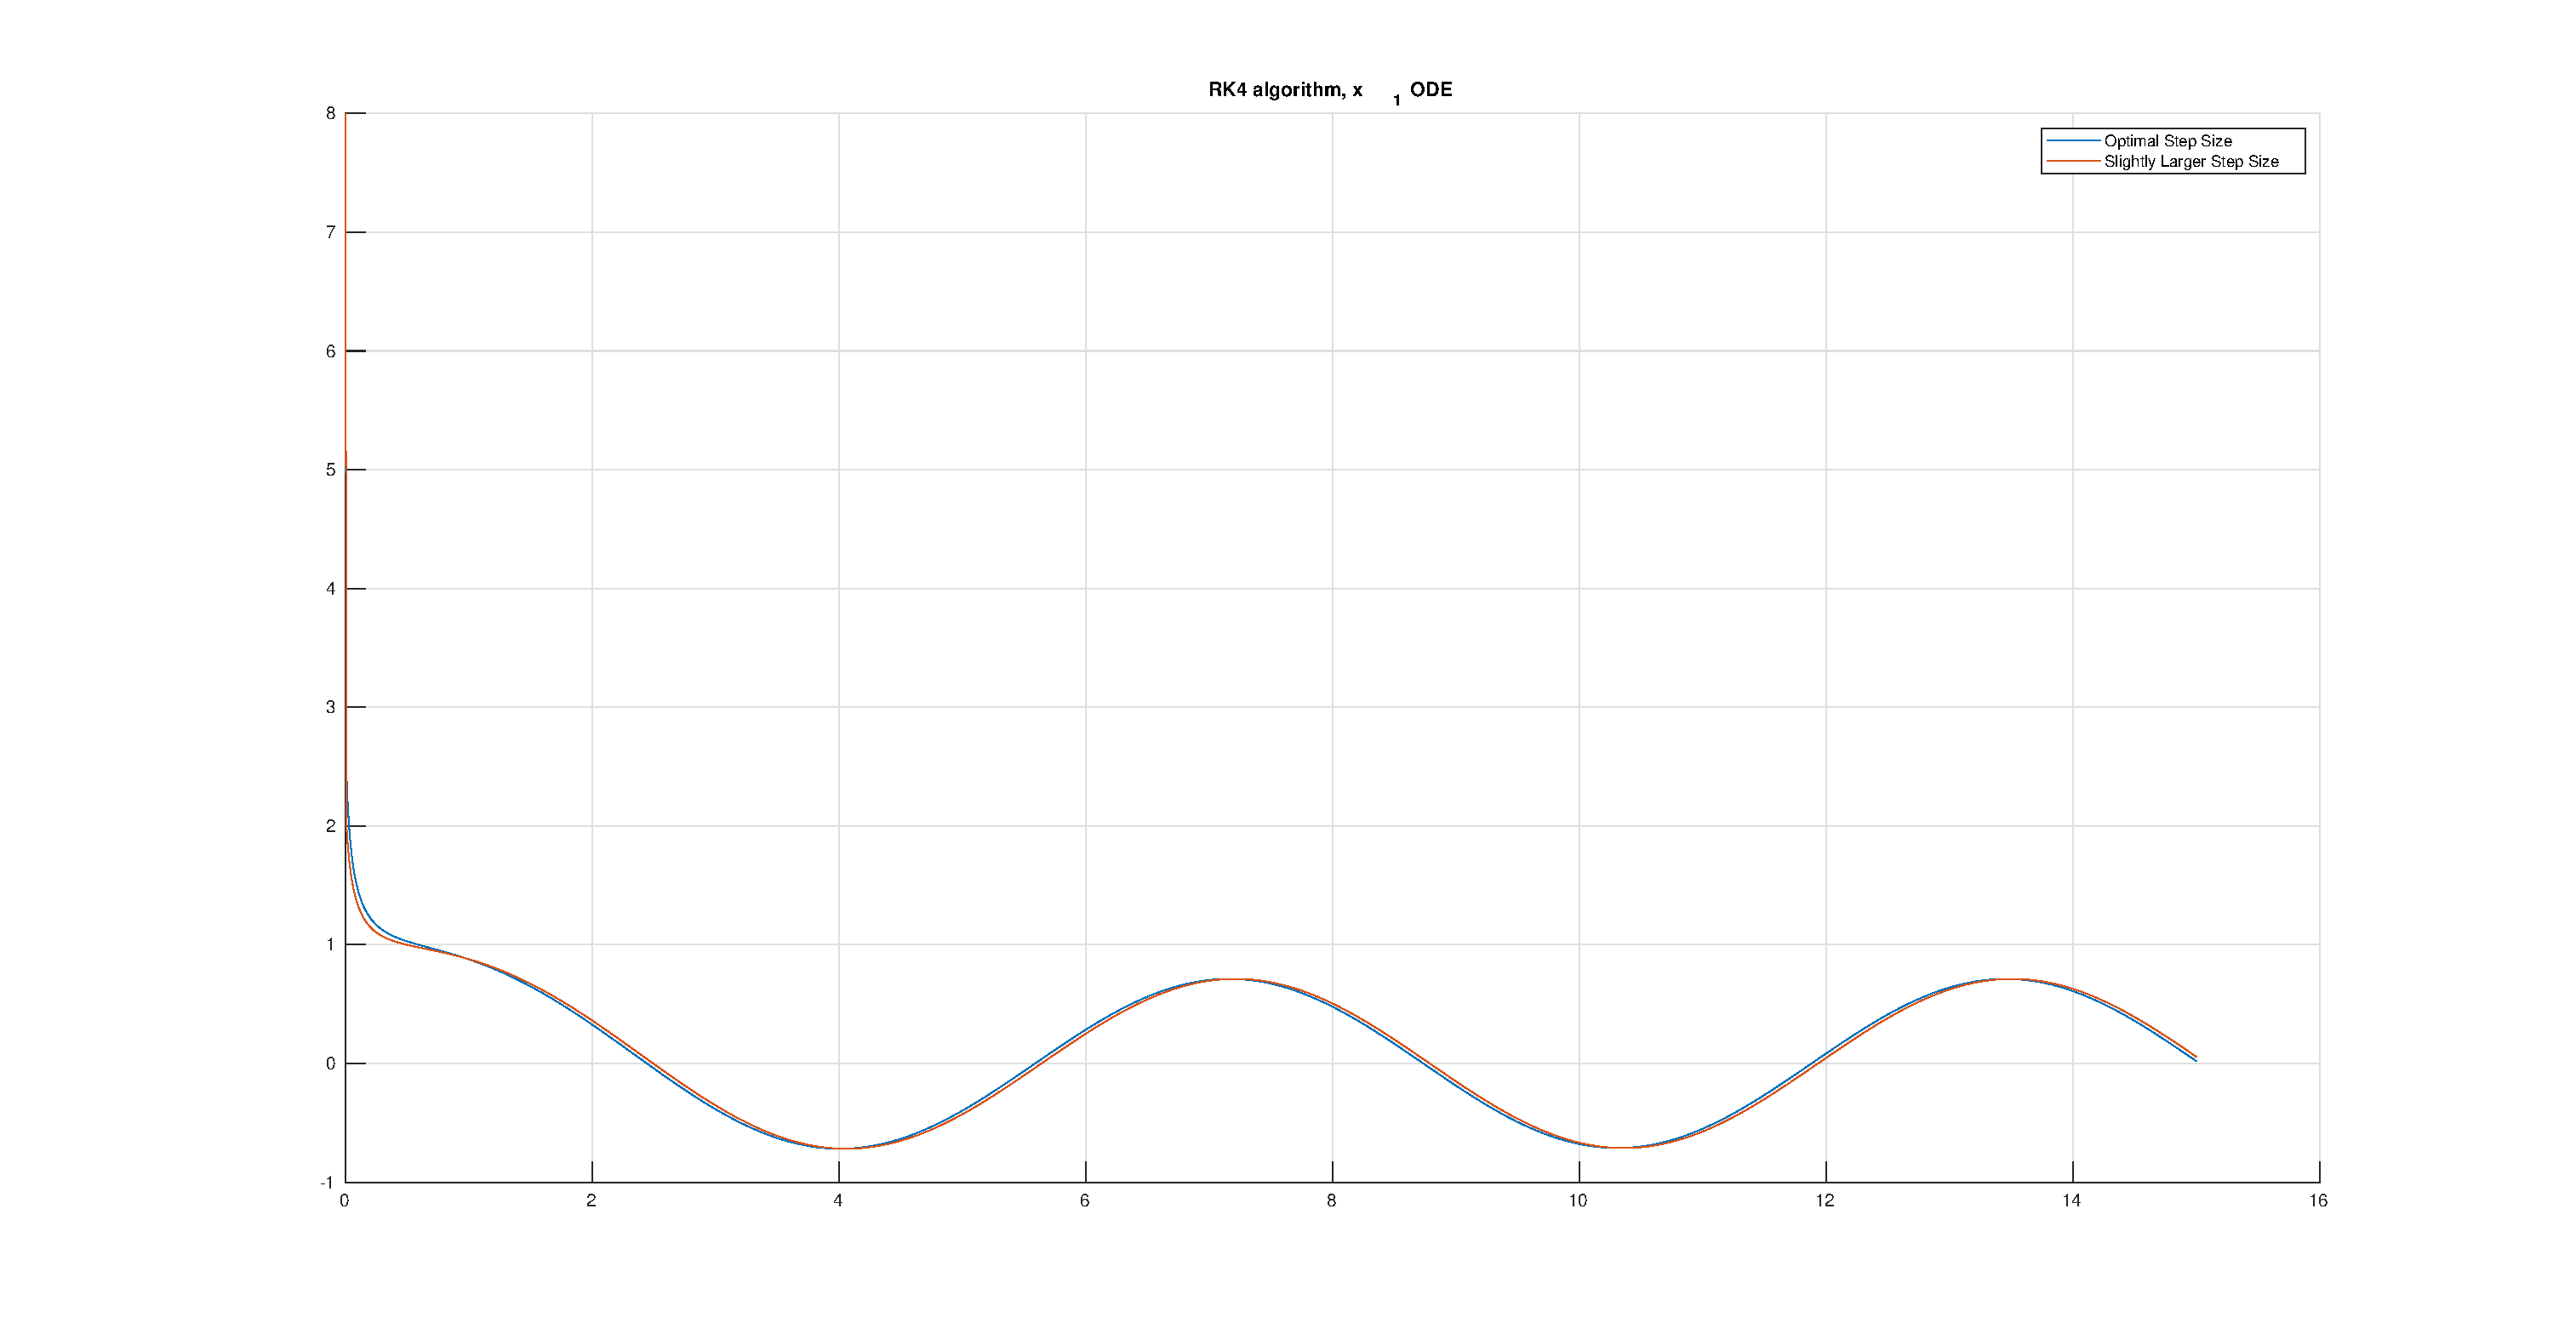
\includegraphics[scale=0.25]{20.eps}
\end{center}

\begin{center}
   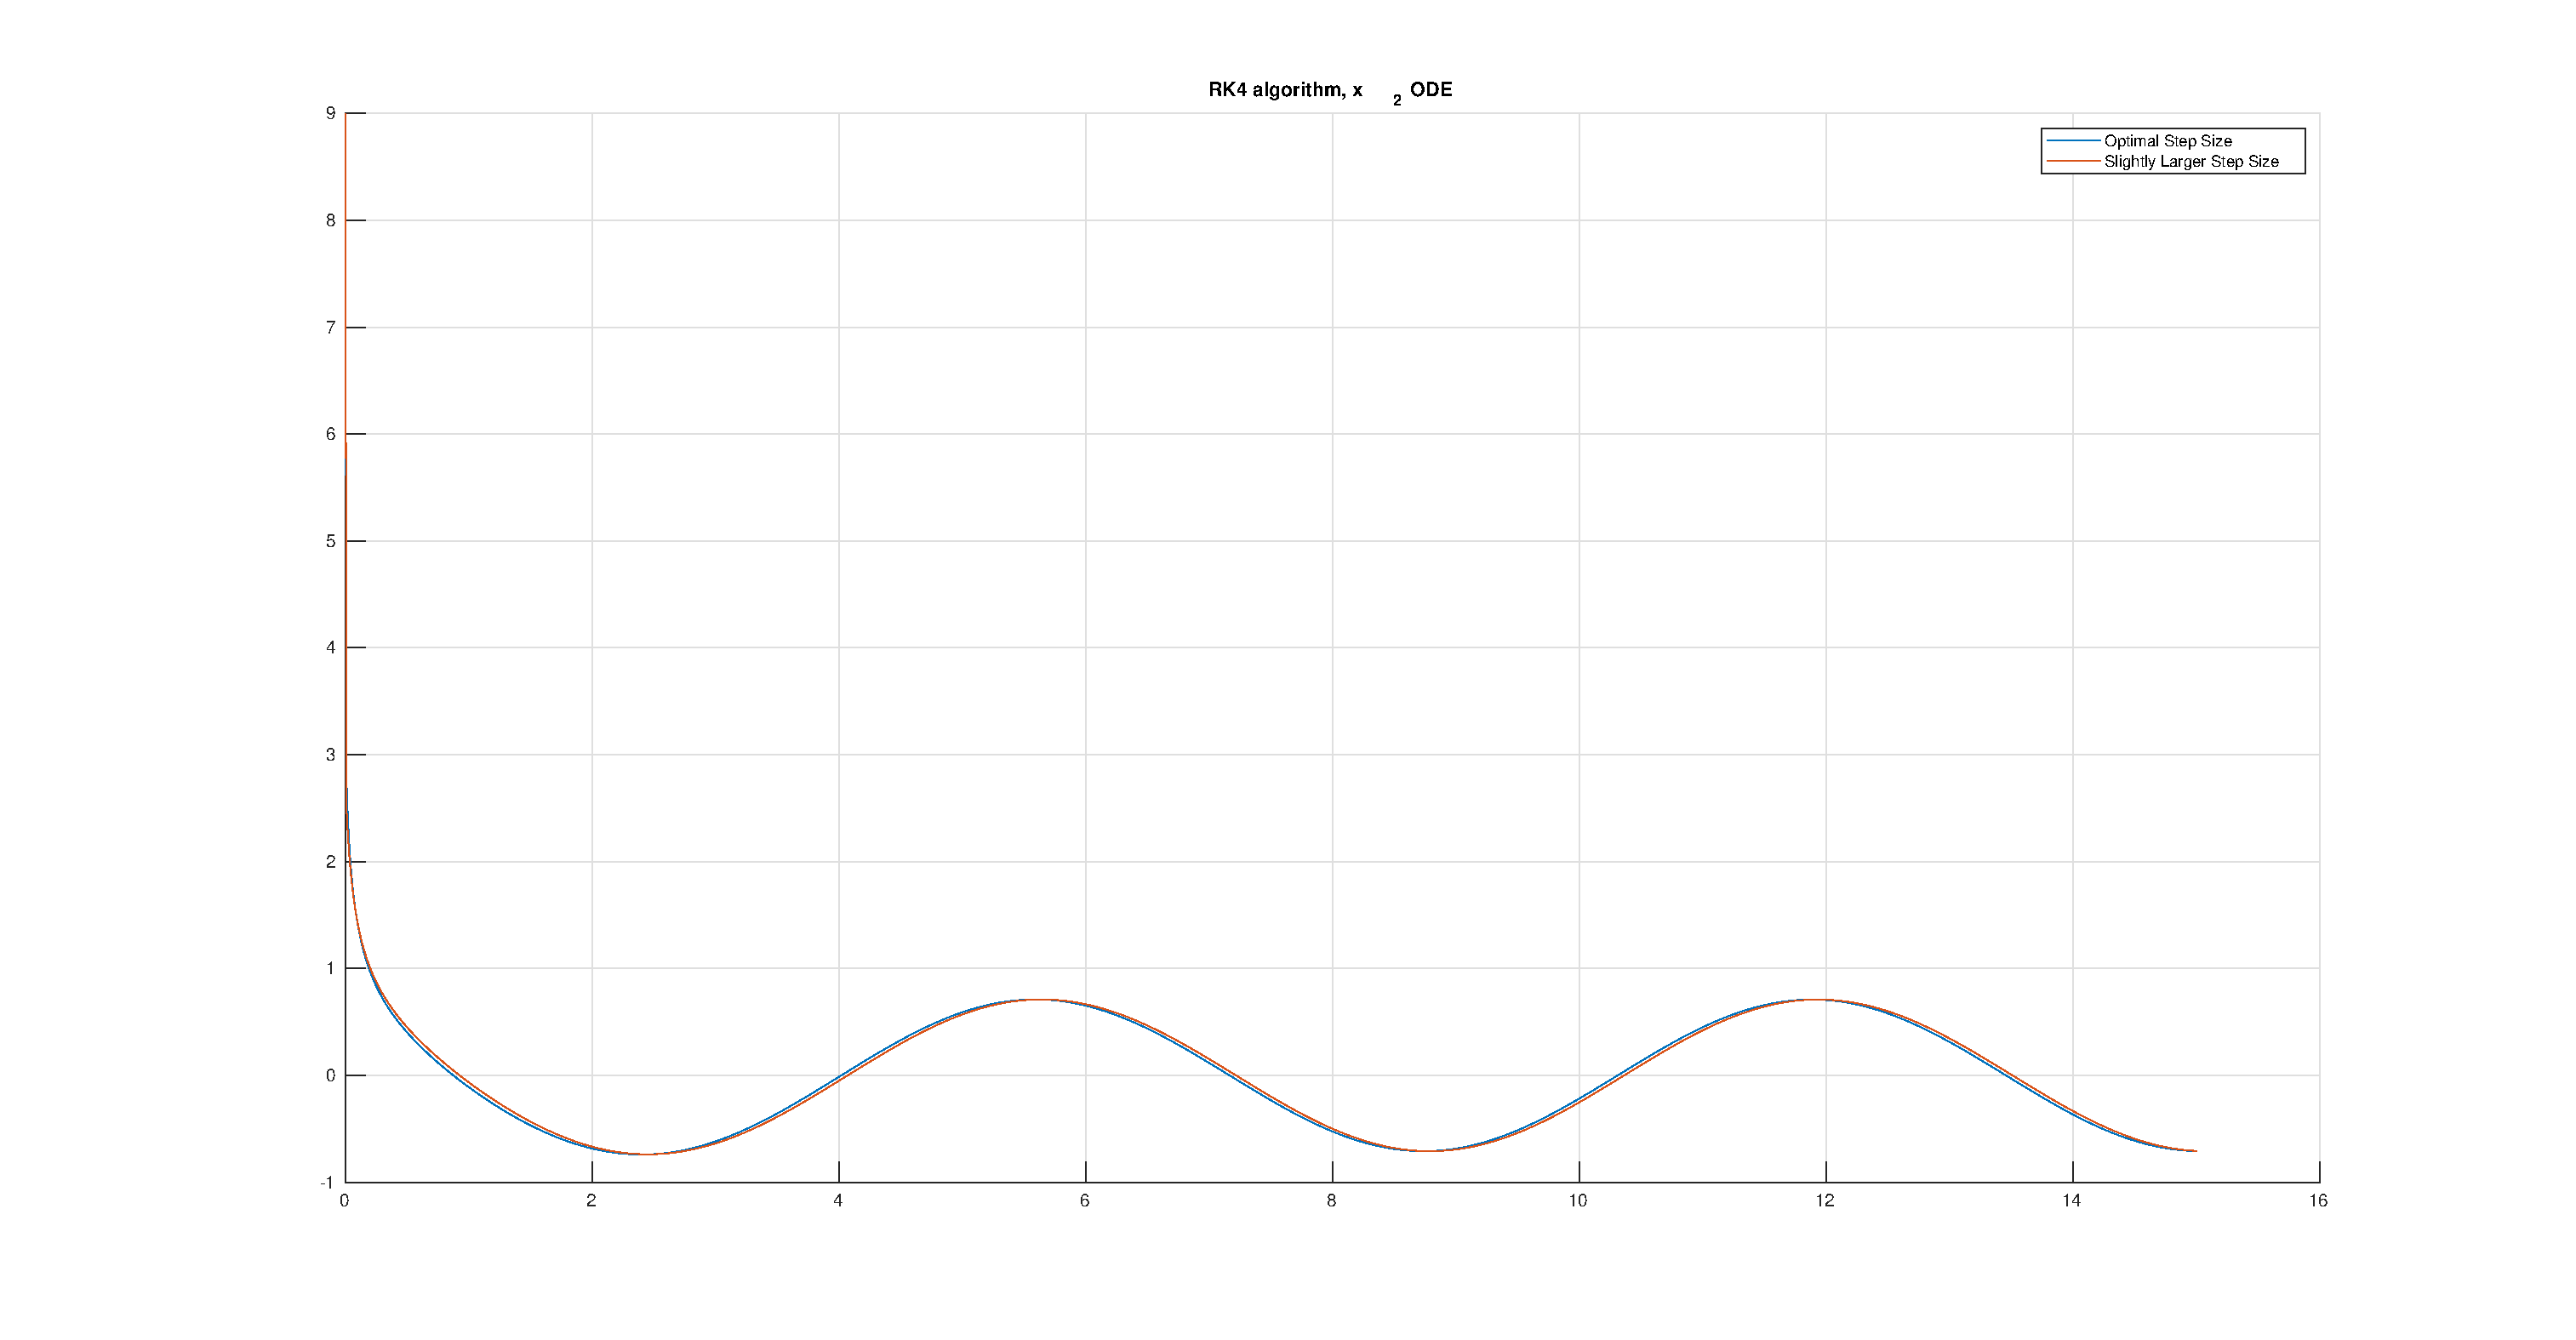
\includegraphics[scale=0.25]{21.eps}
\end{center}

\begin{center}
   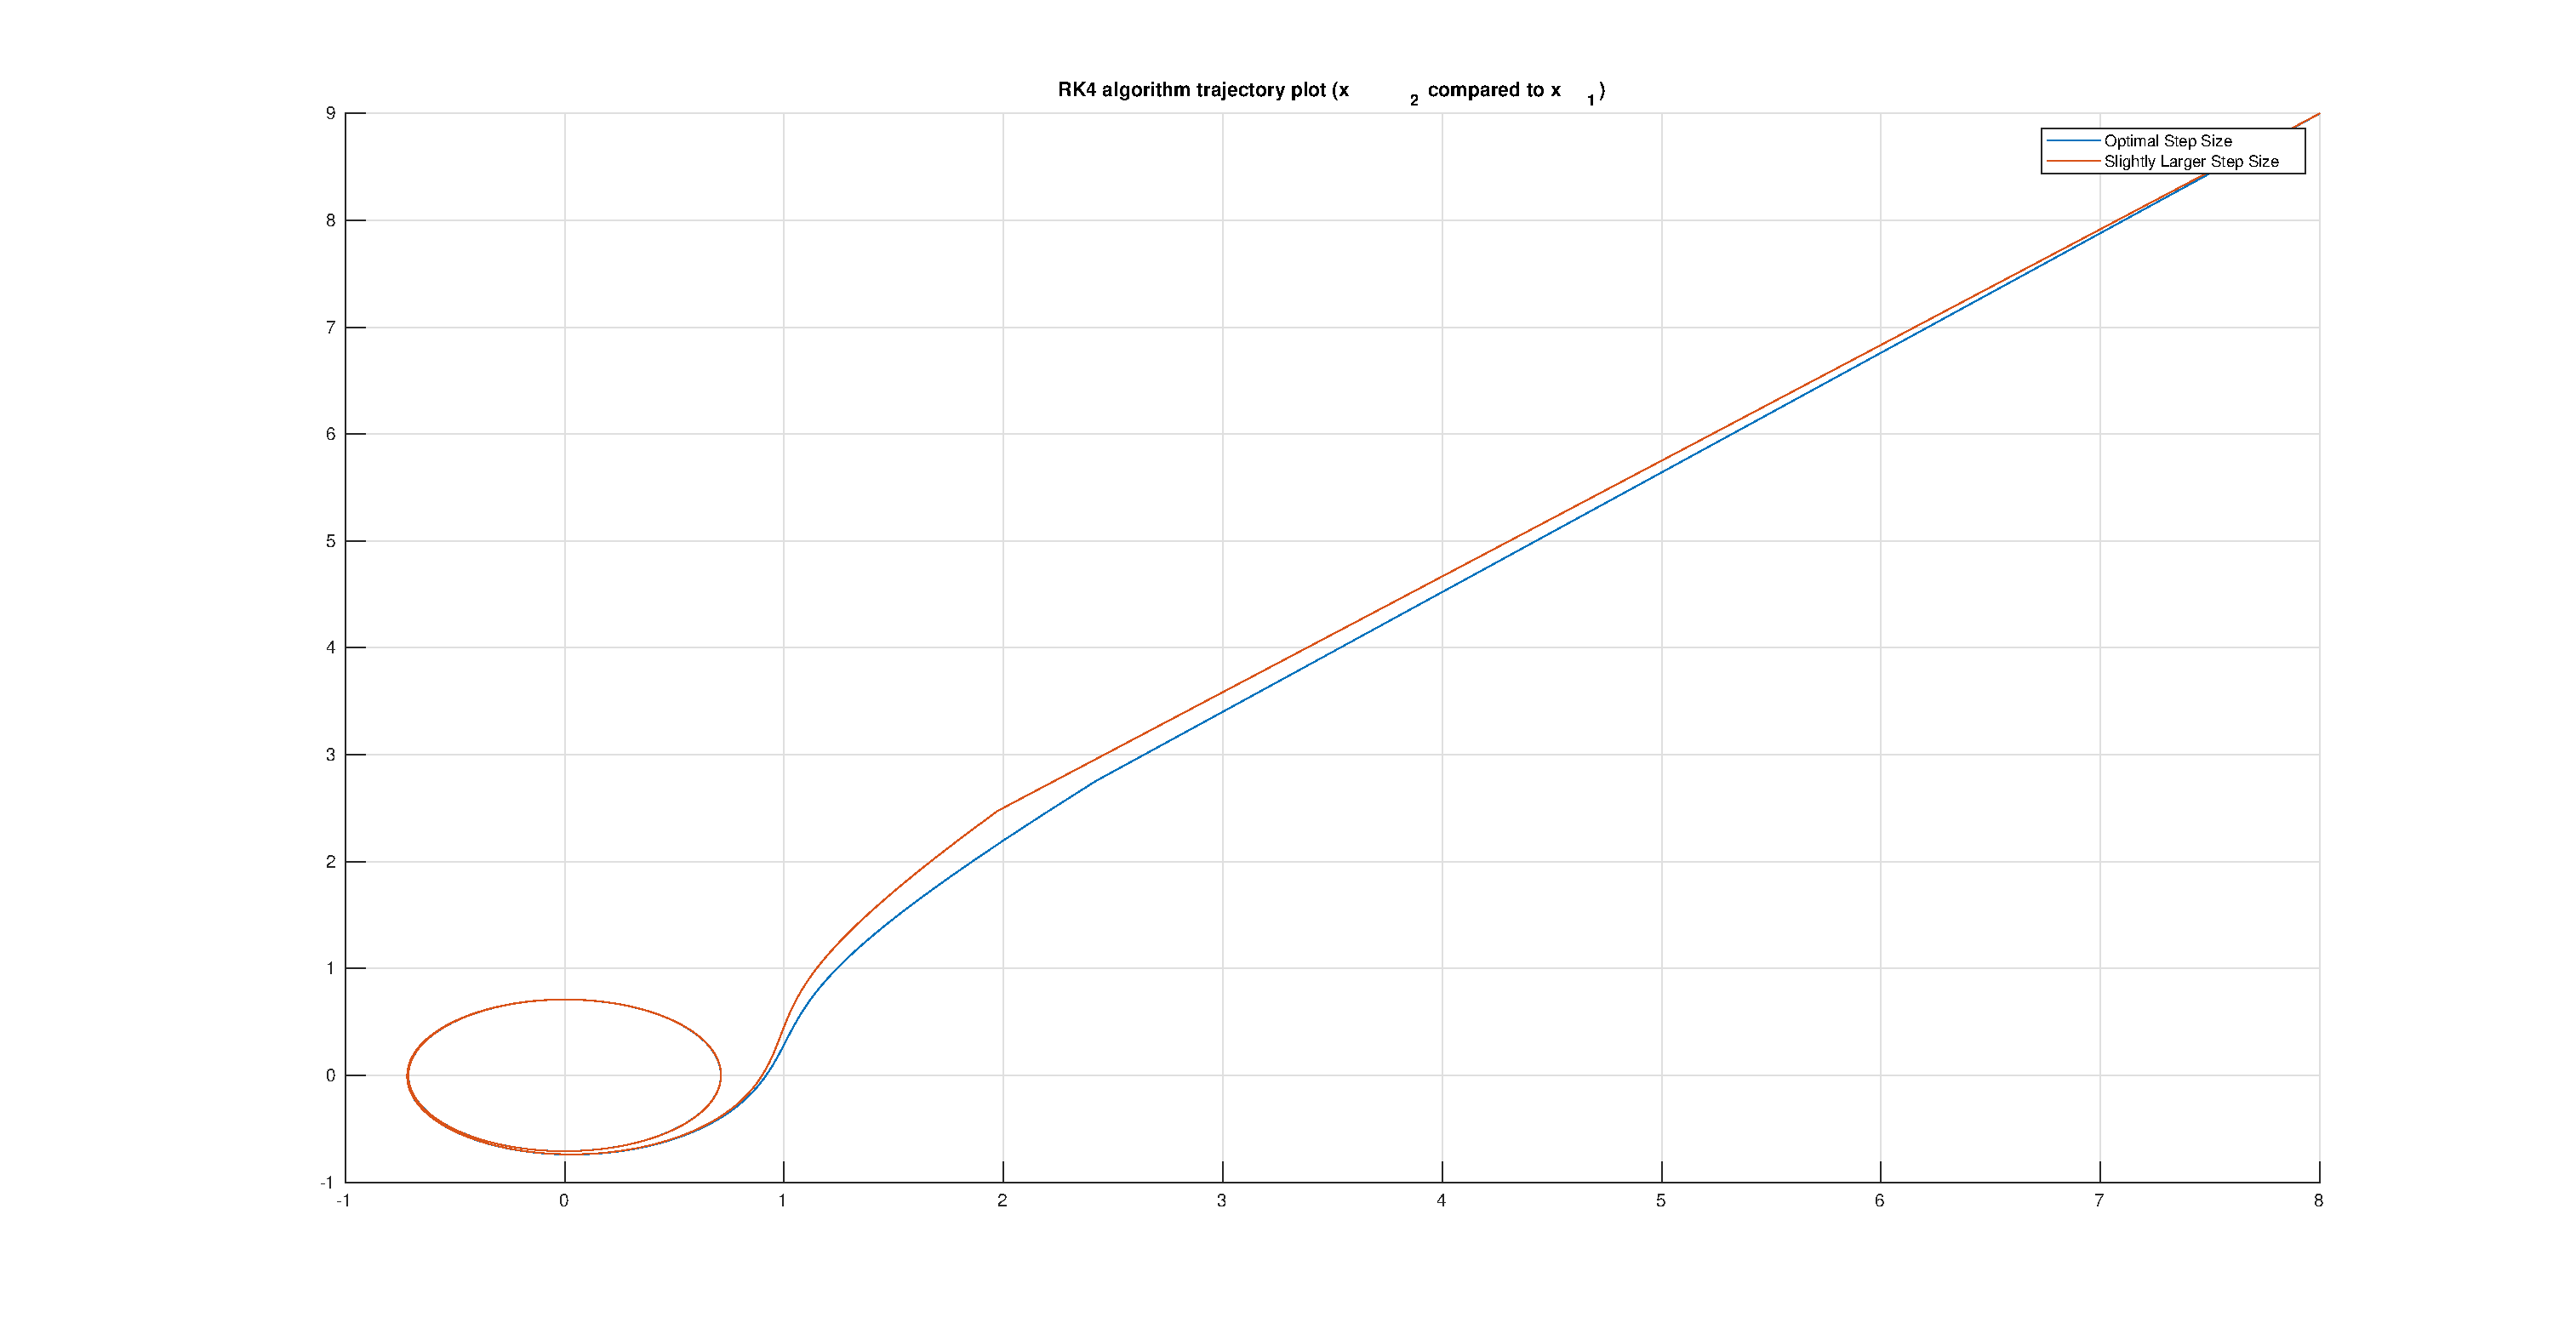
\includegraphics[scale=0.25]{22.eps}
\end{center}

\begin{center}
   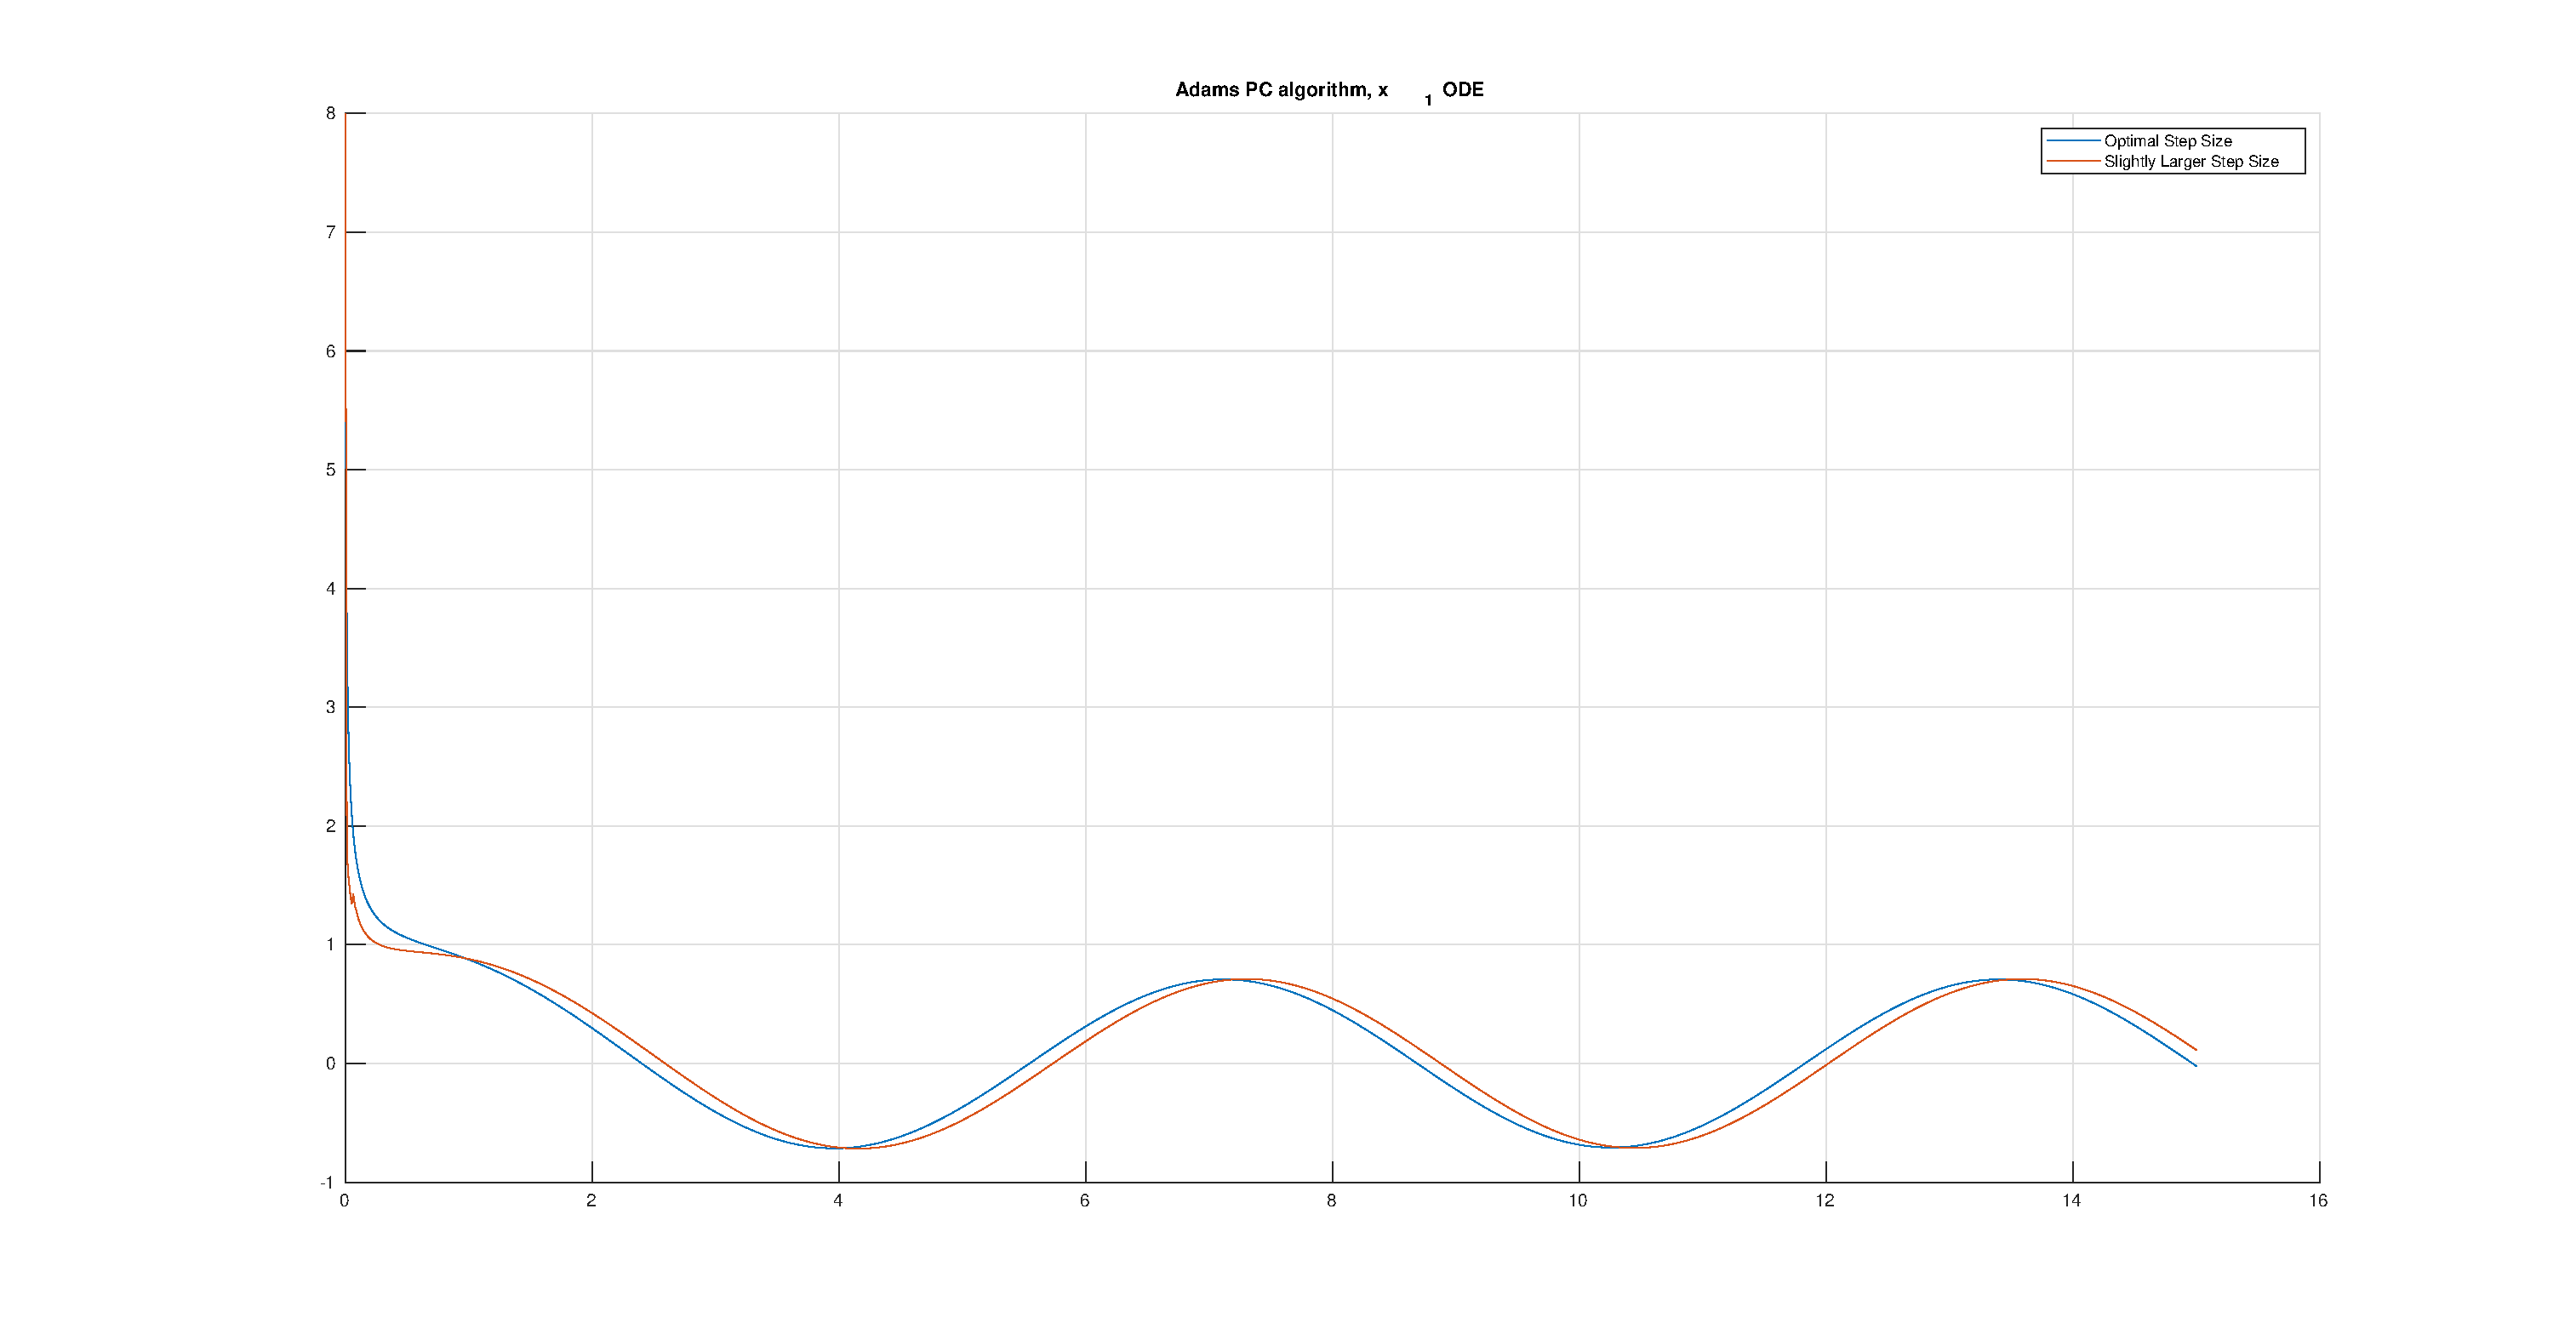
\includegraphics[scale=0.25]{23.eps}
\end{center}

\begin{center}
   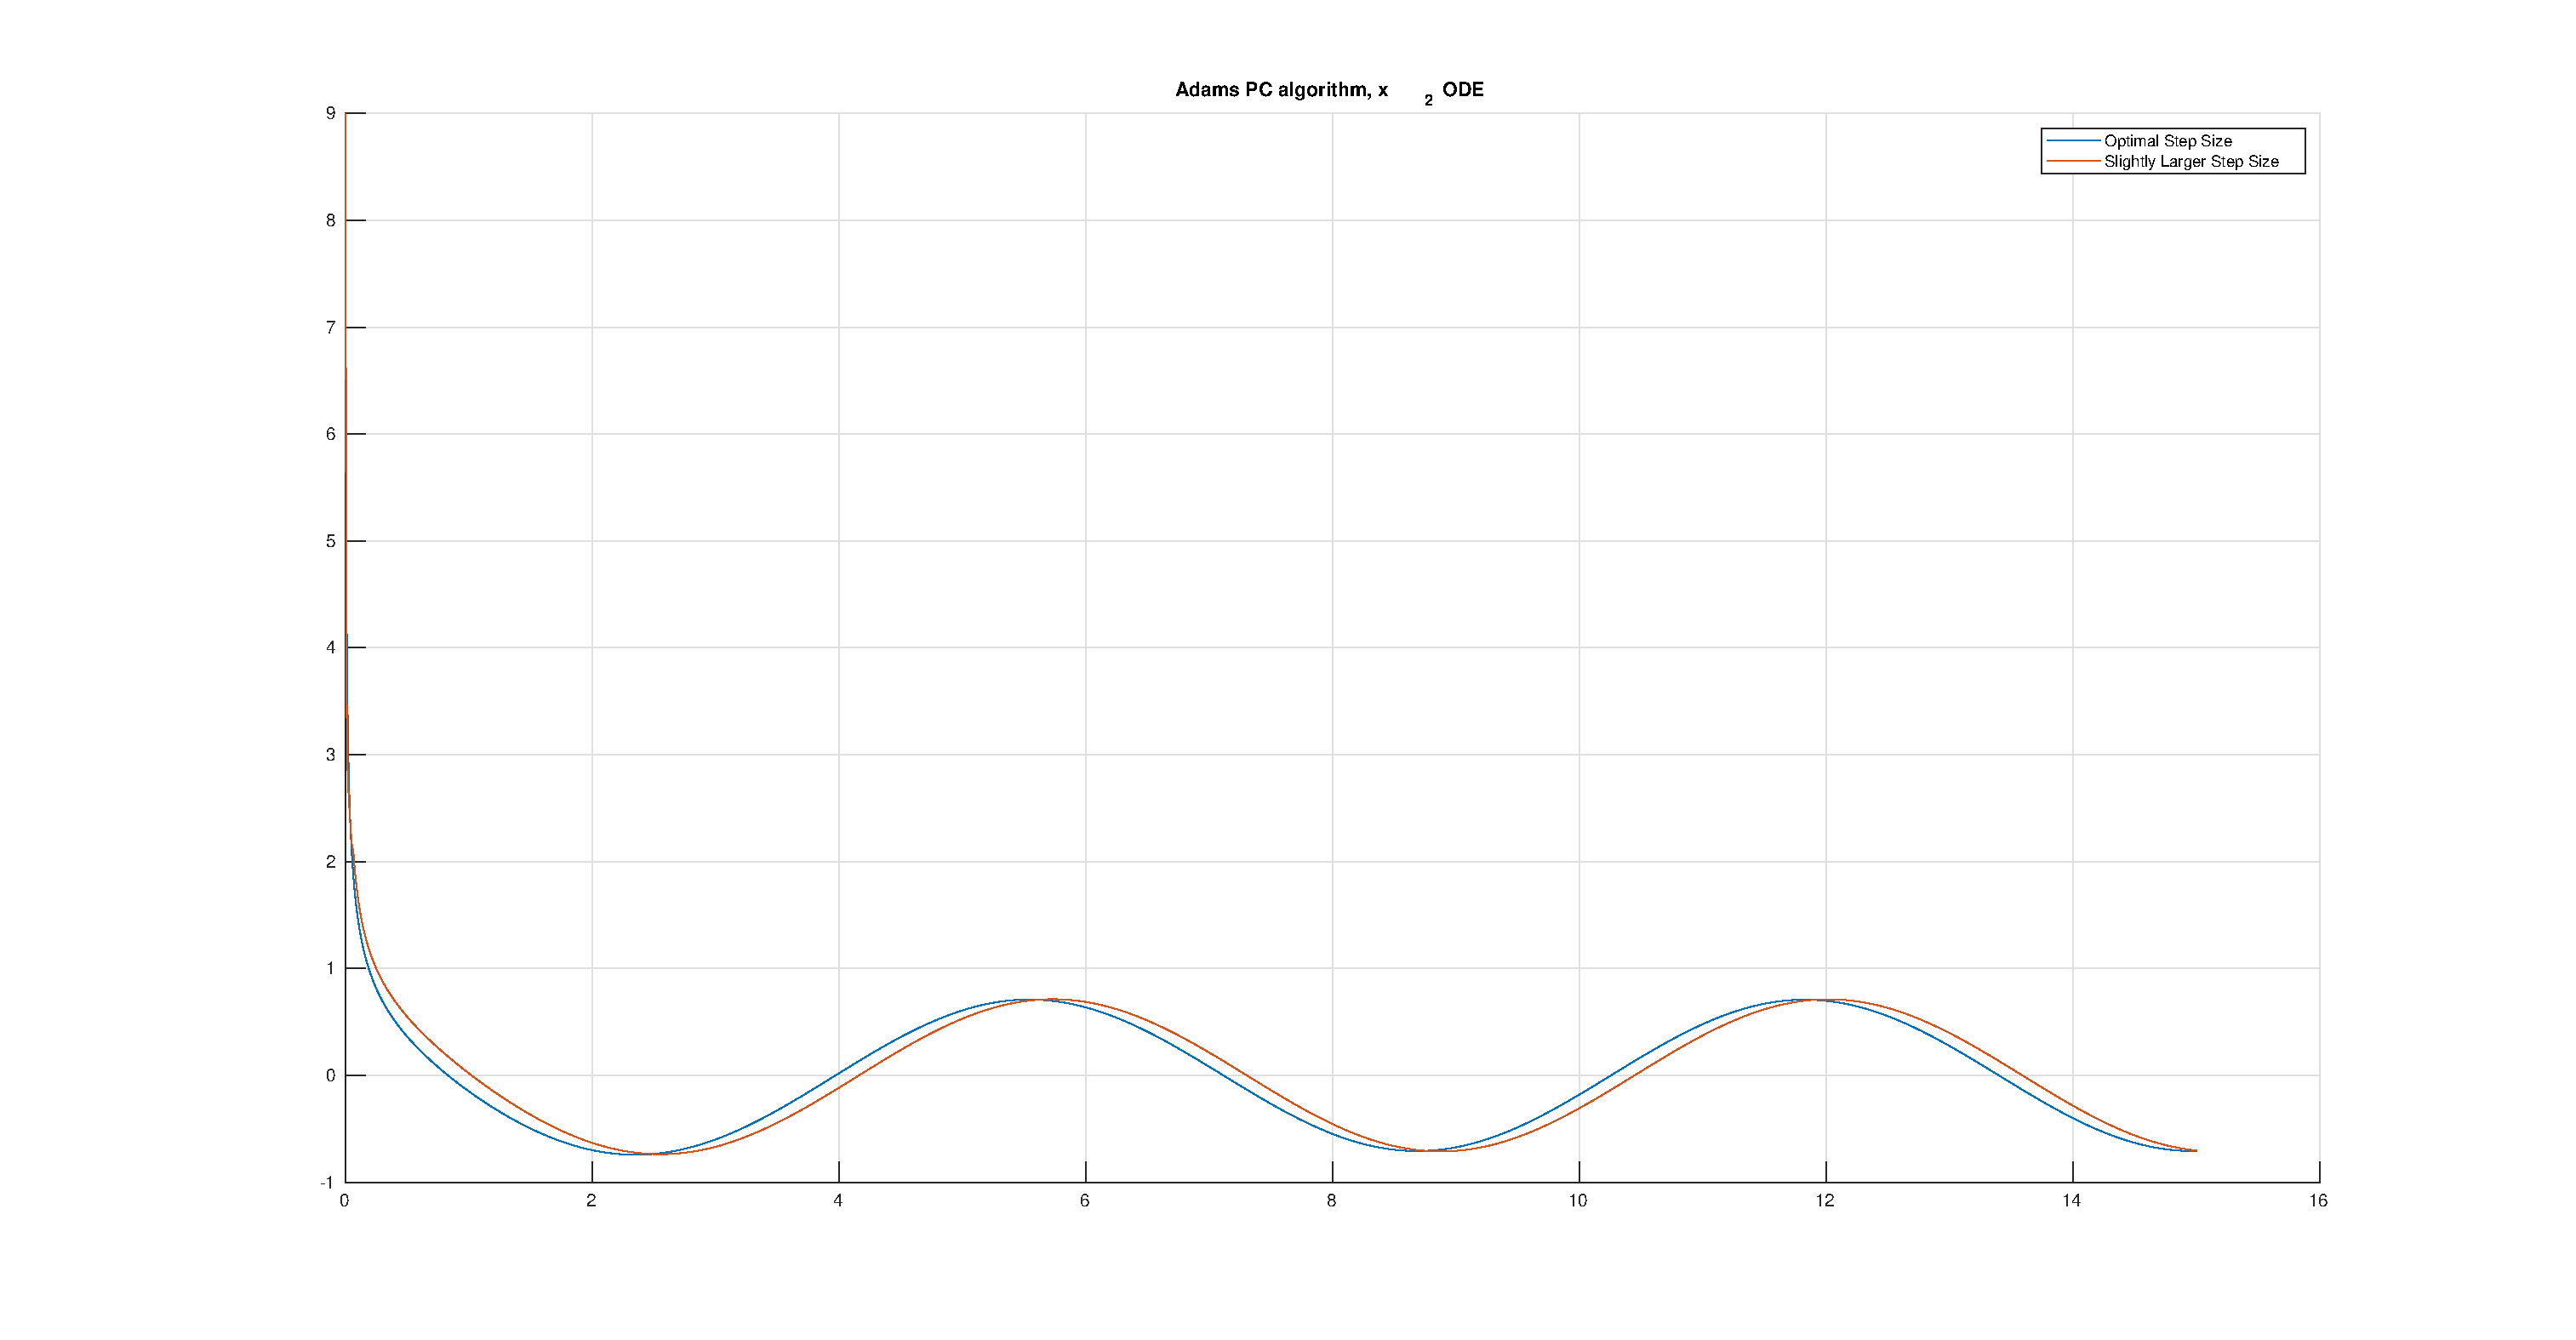
\includegraphics[scale=0.25]{24.eps}
\end{center}

\begin{center}
   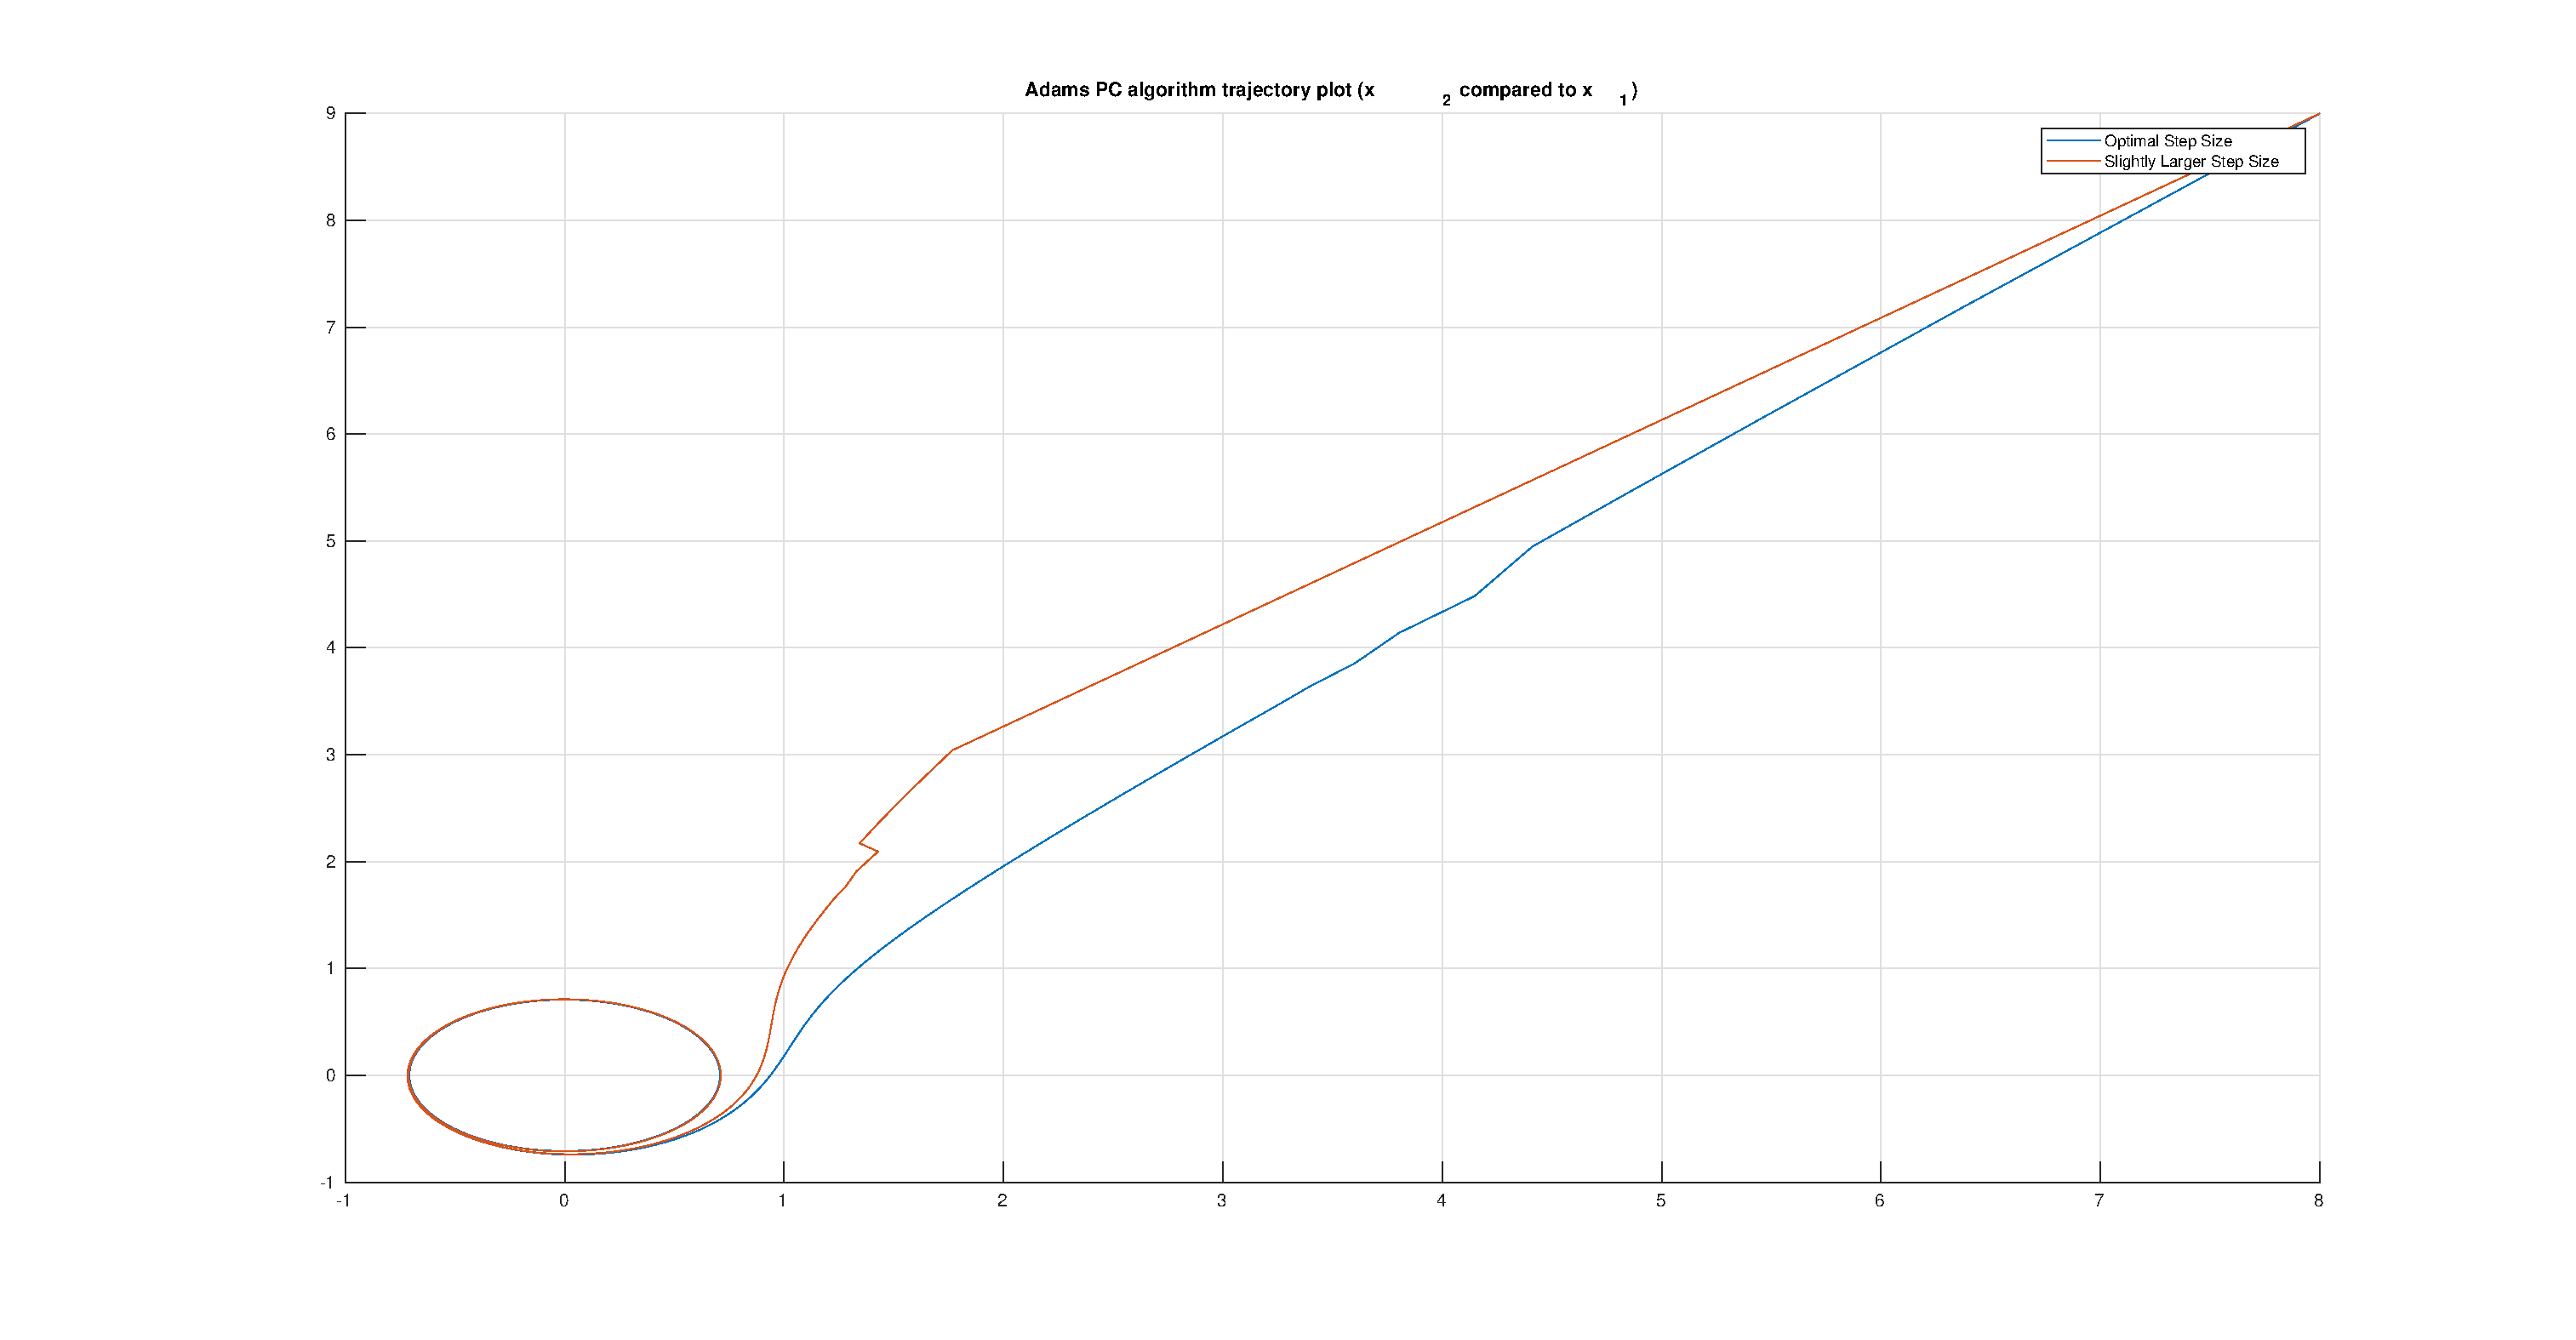
\includegraphics[scale=0.25]{25.eps}
\end{center}

\begin{center}
   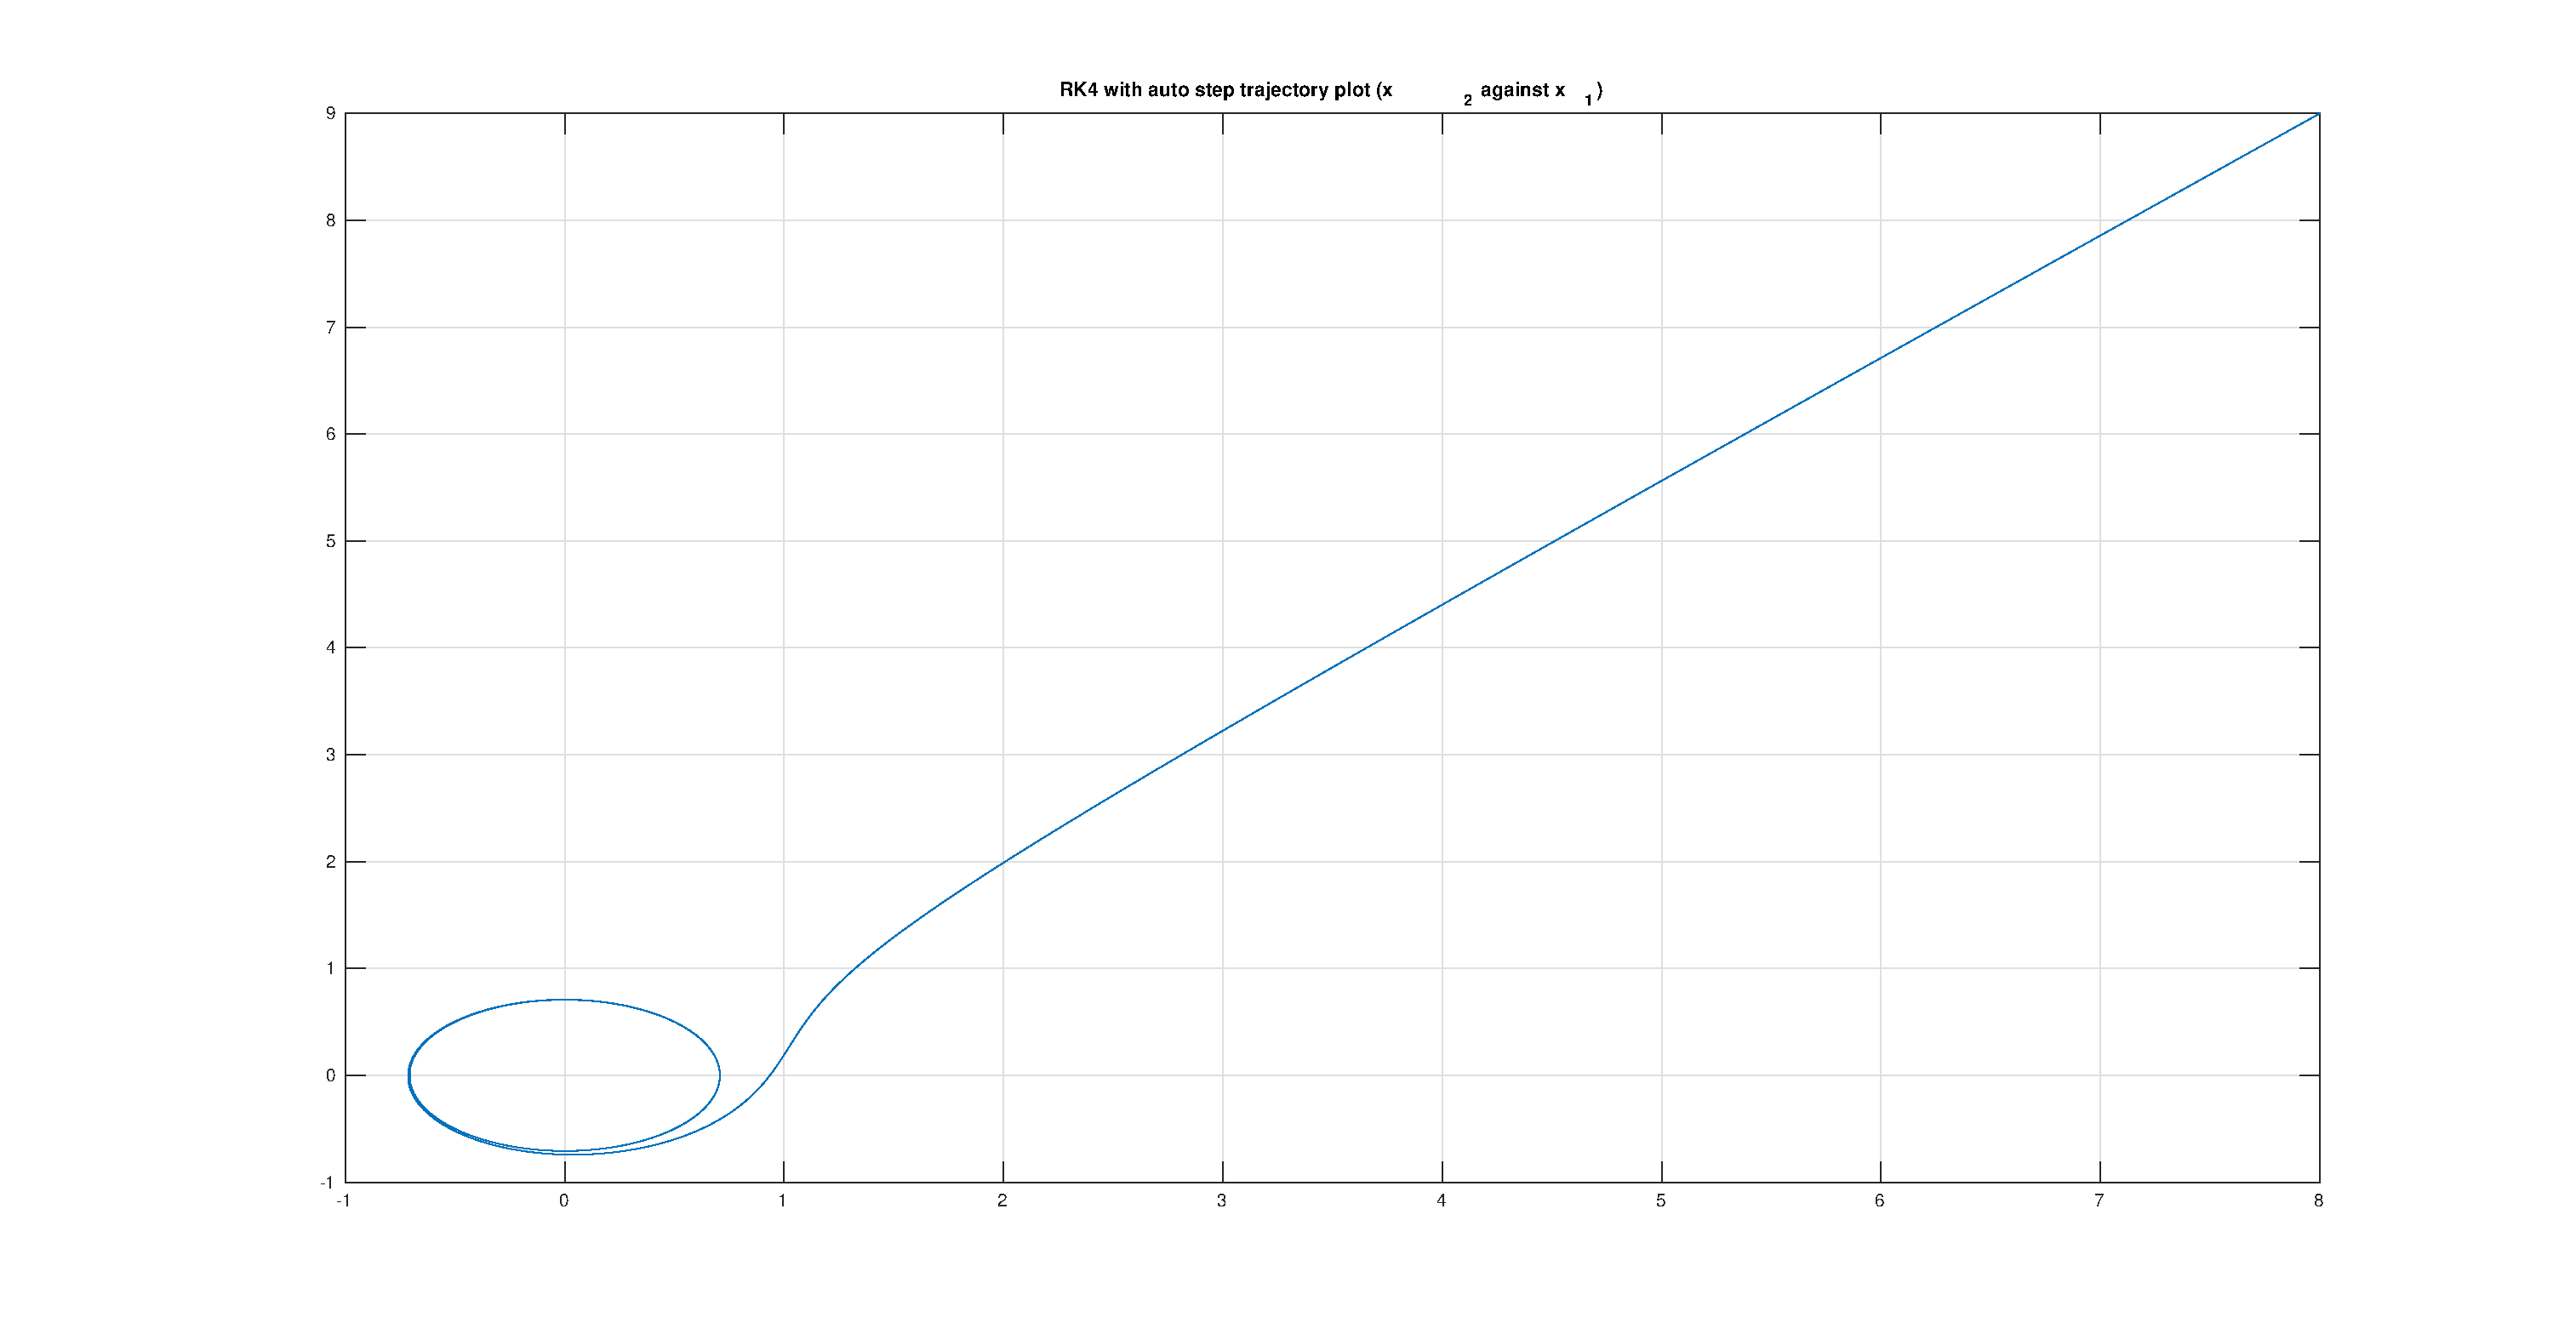
\includegraphics[scale=0.25]{26.eps}
\end{center}

\begin{center}
   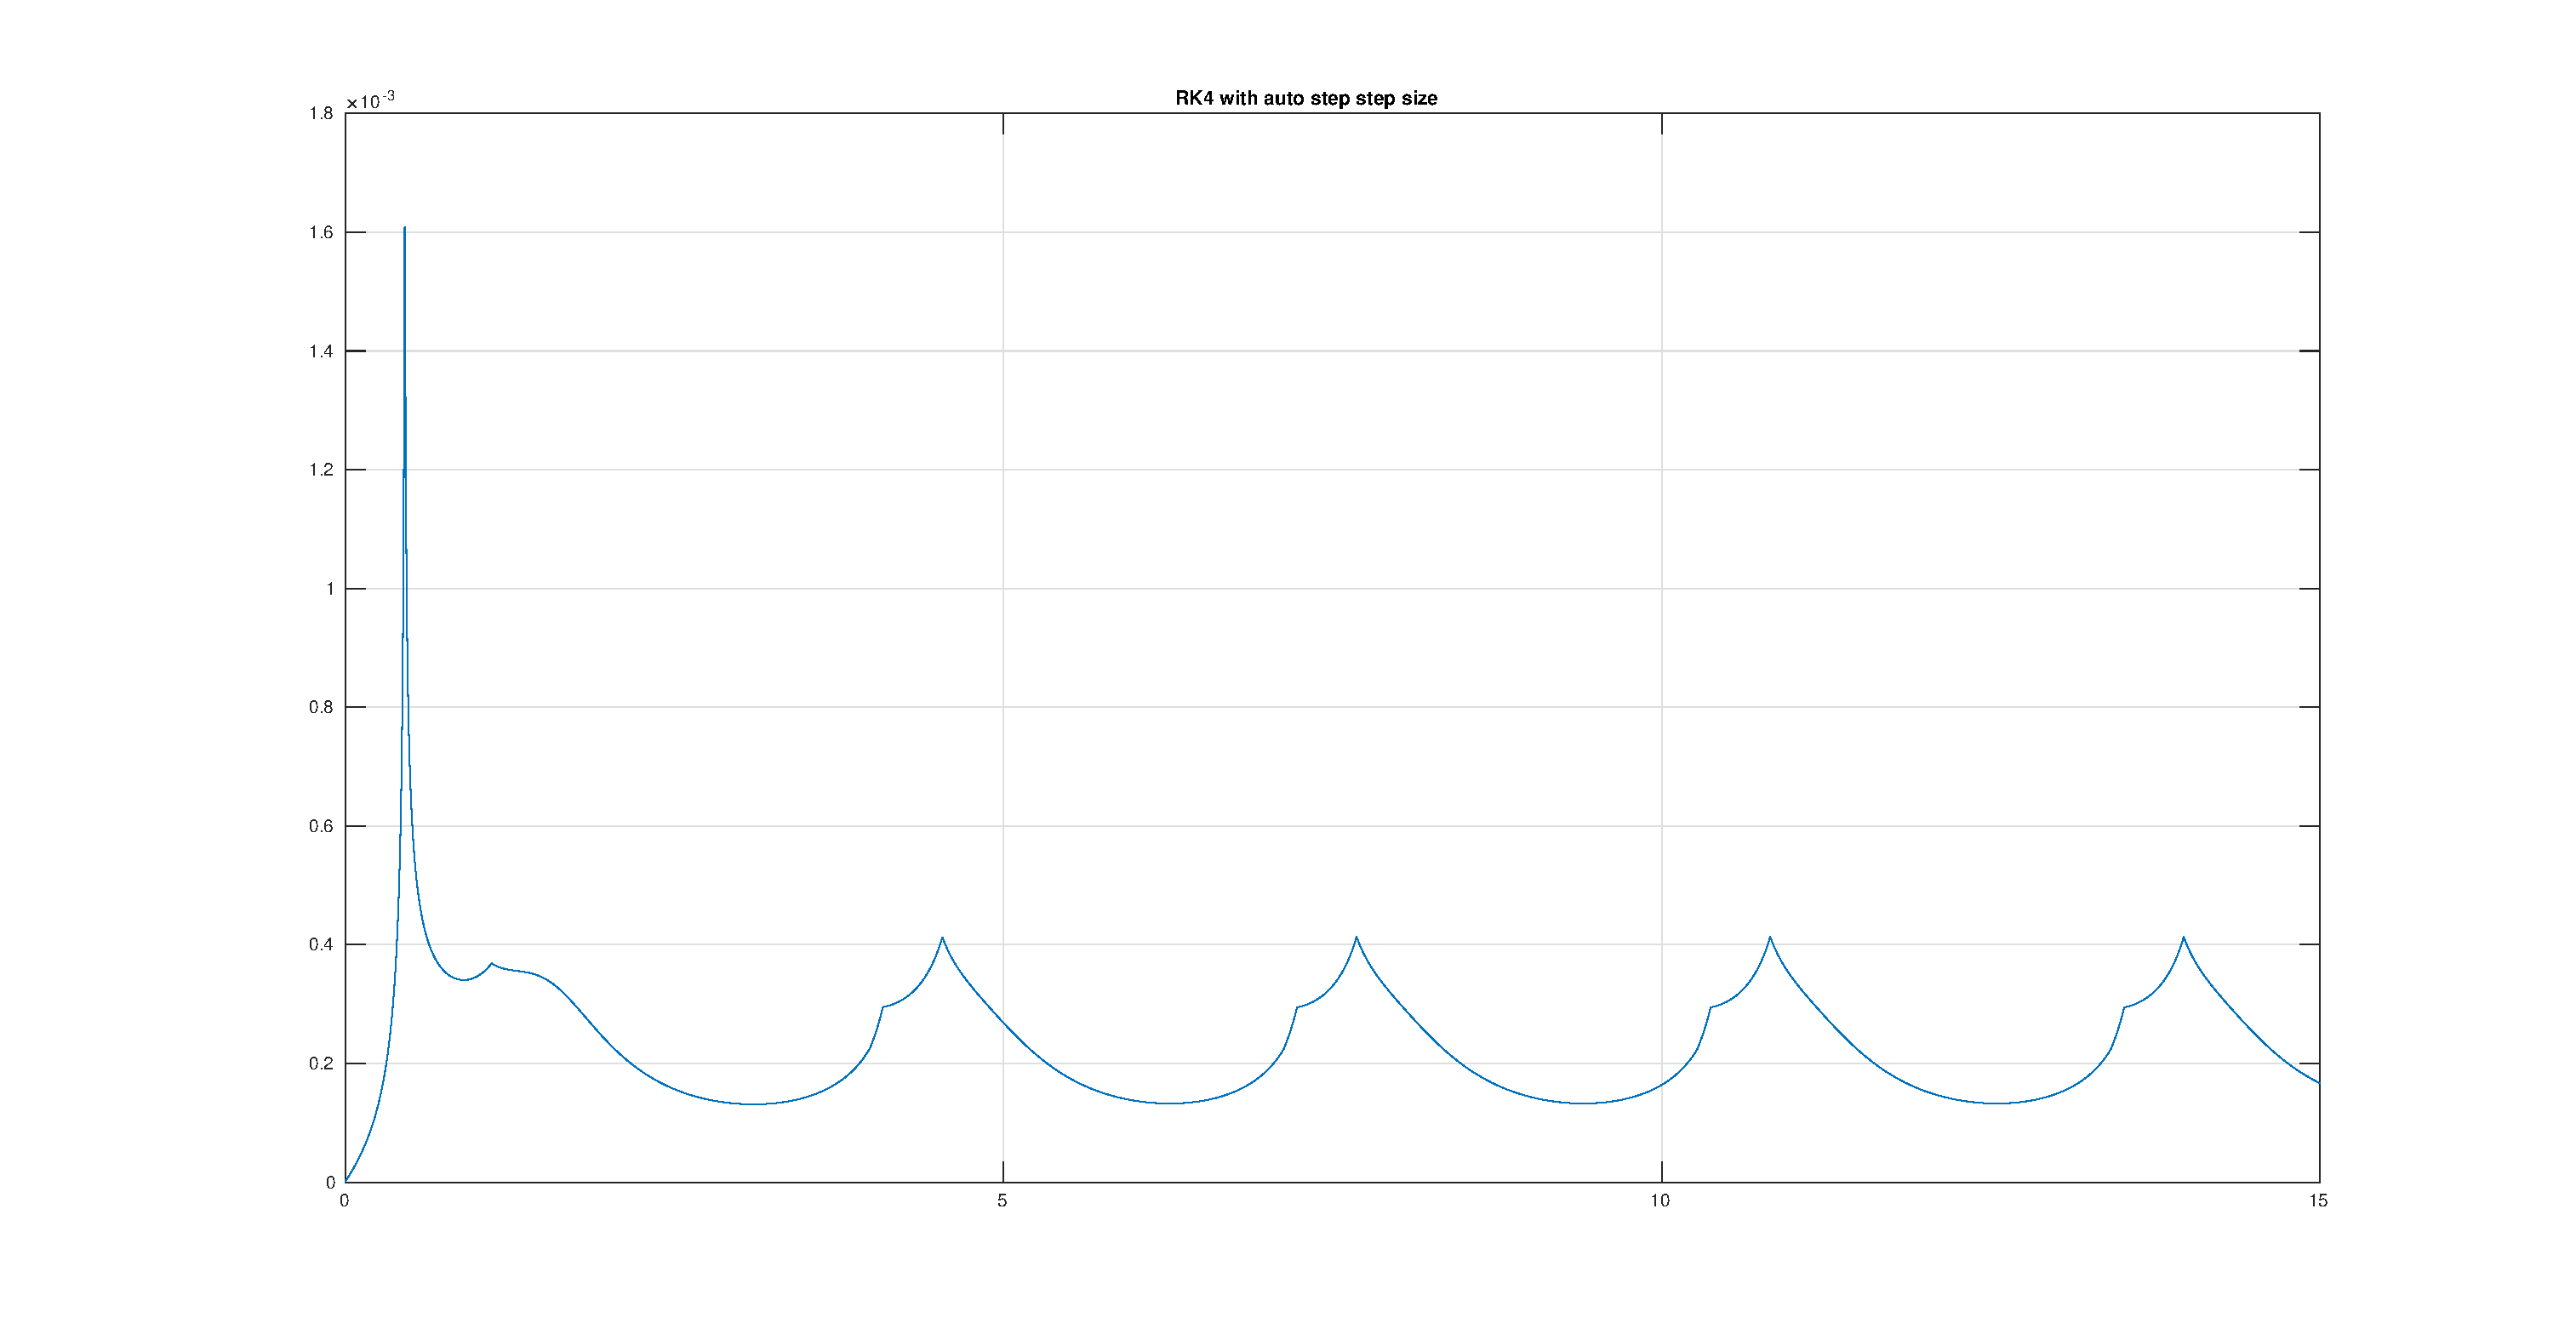
\includegraphics[scale=0.25]{27.eps}
\end{center}

\begin{center}
   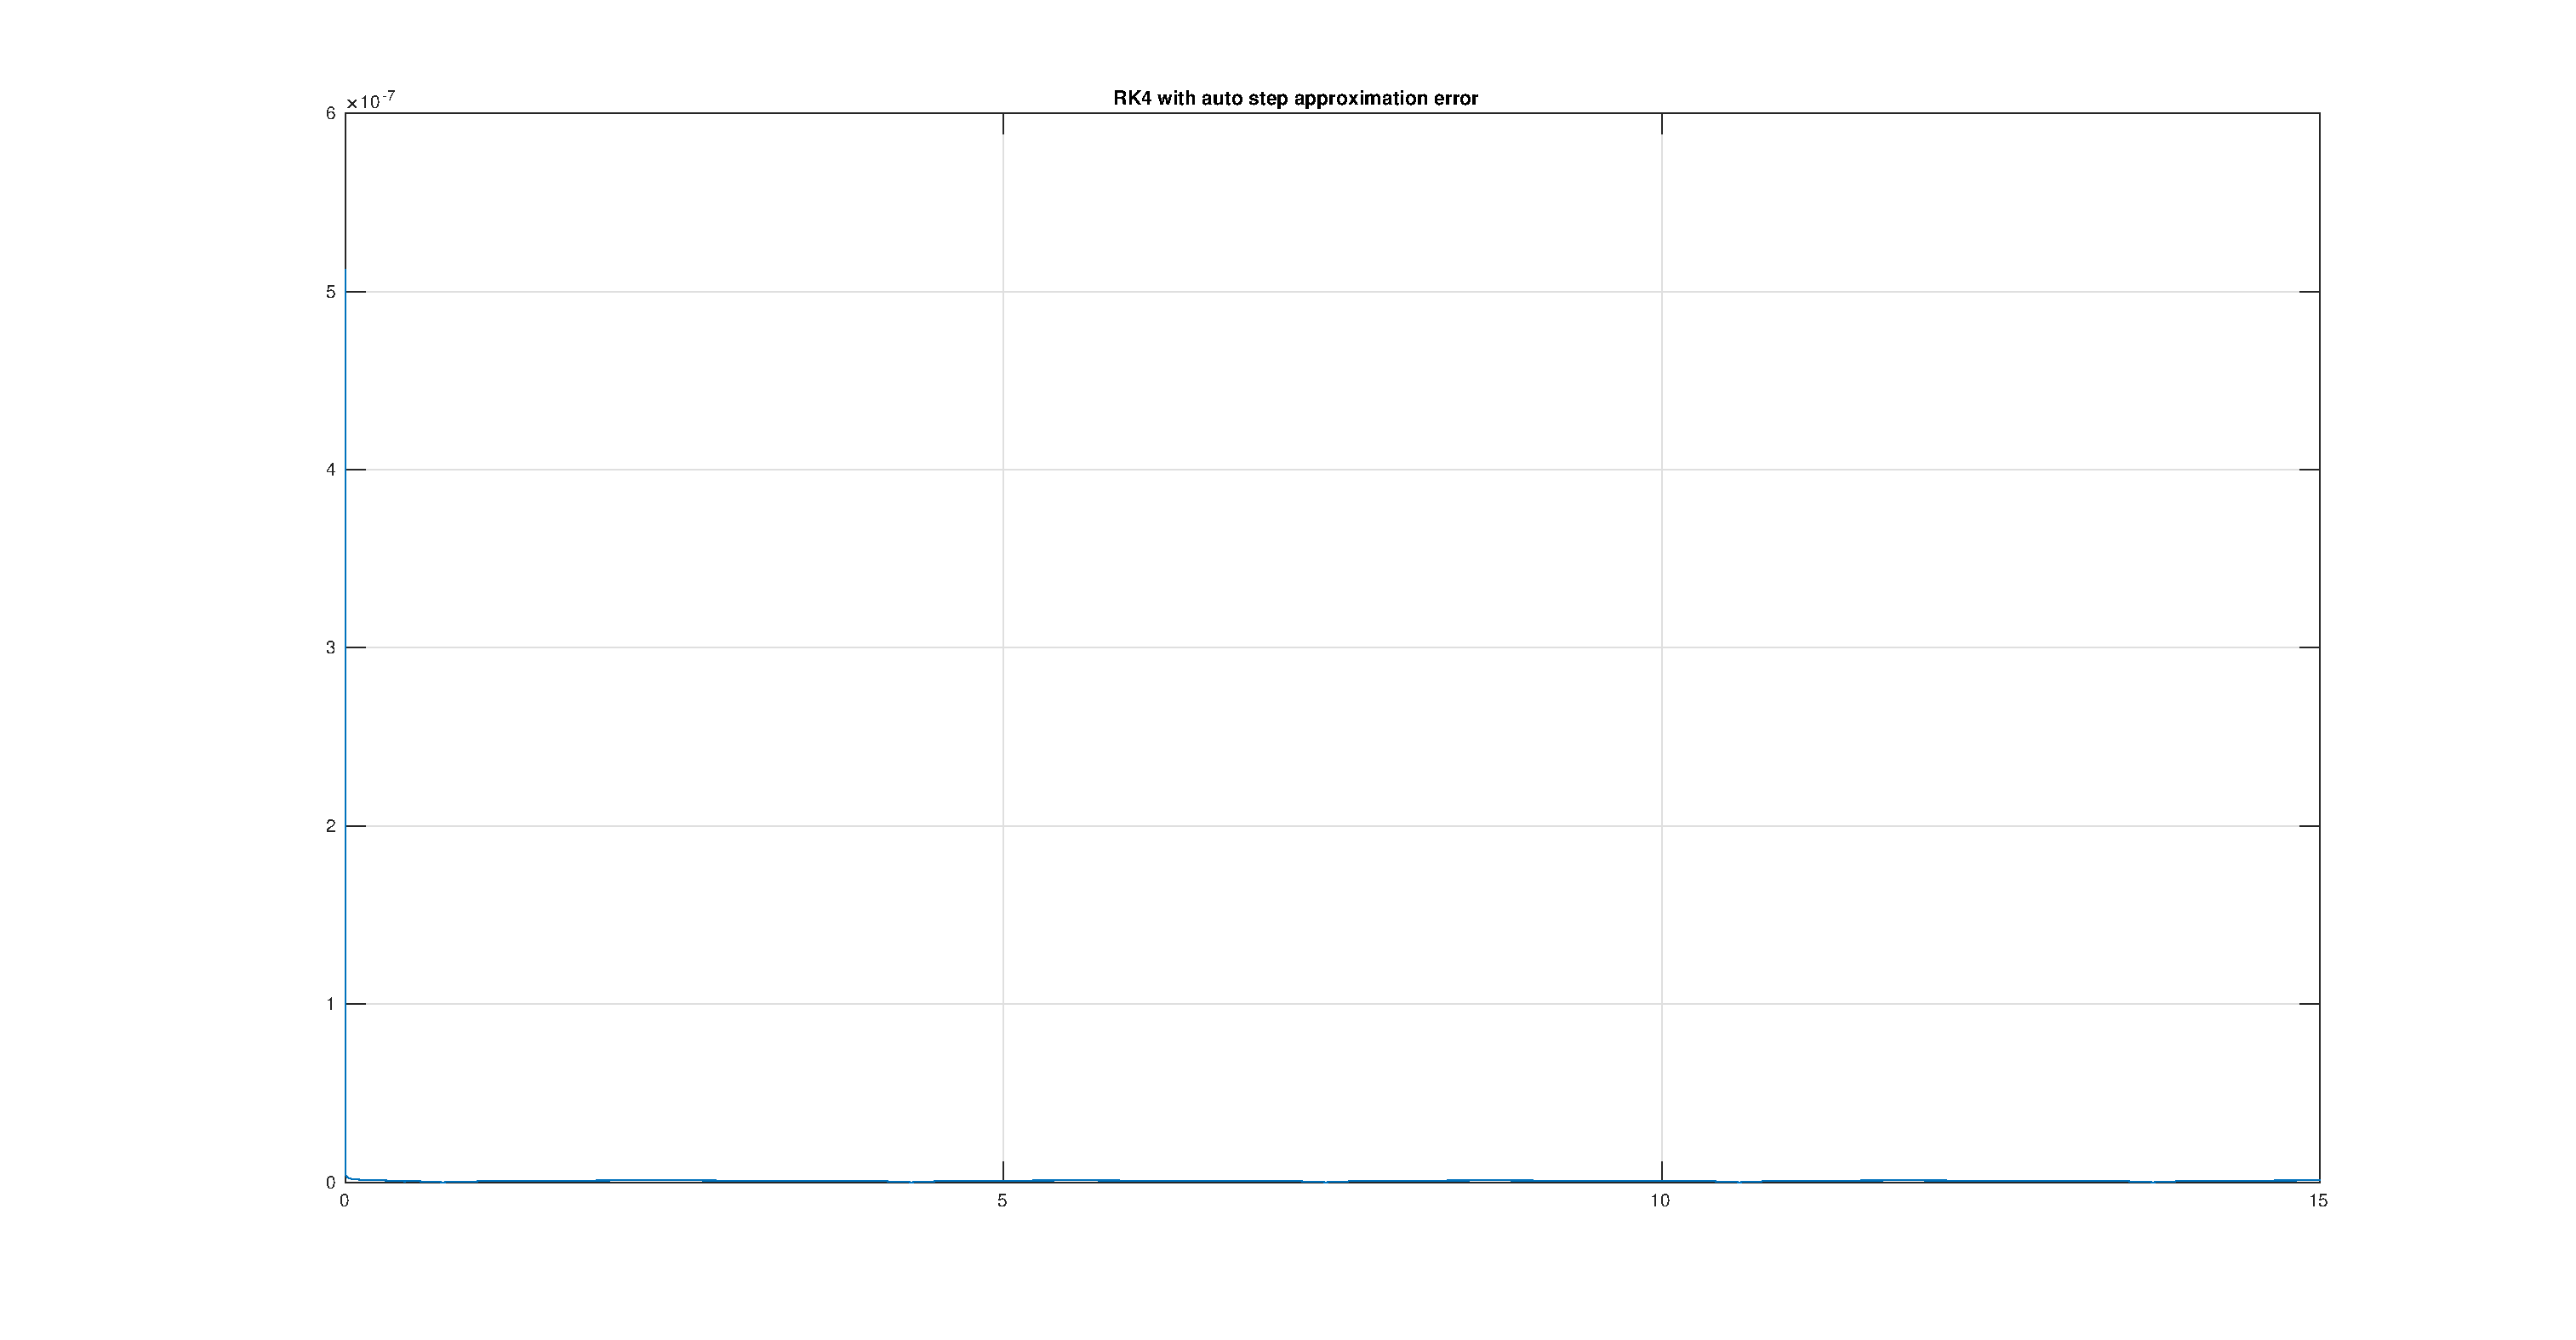
\includegraphics[scale=0.25]{28.eps}
\end{center}

\begin{center}
   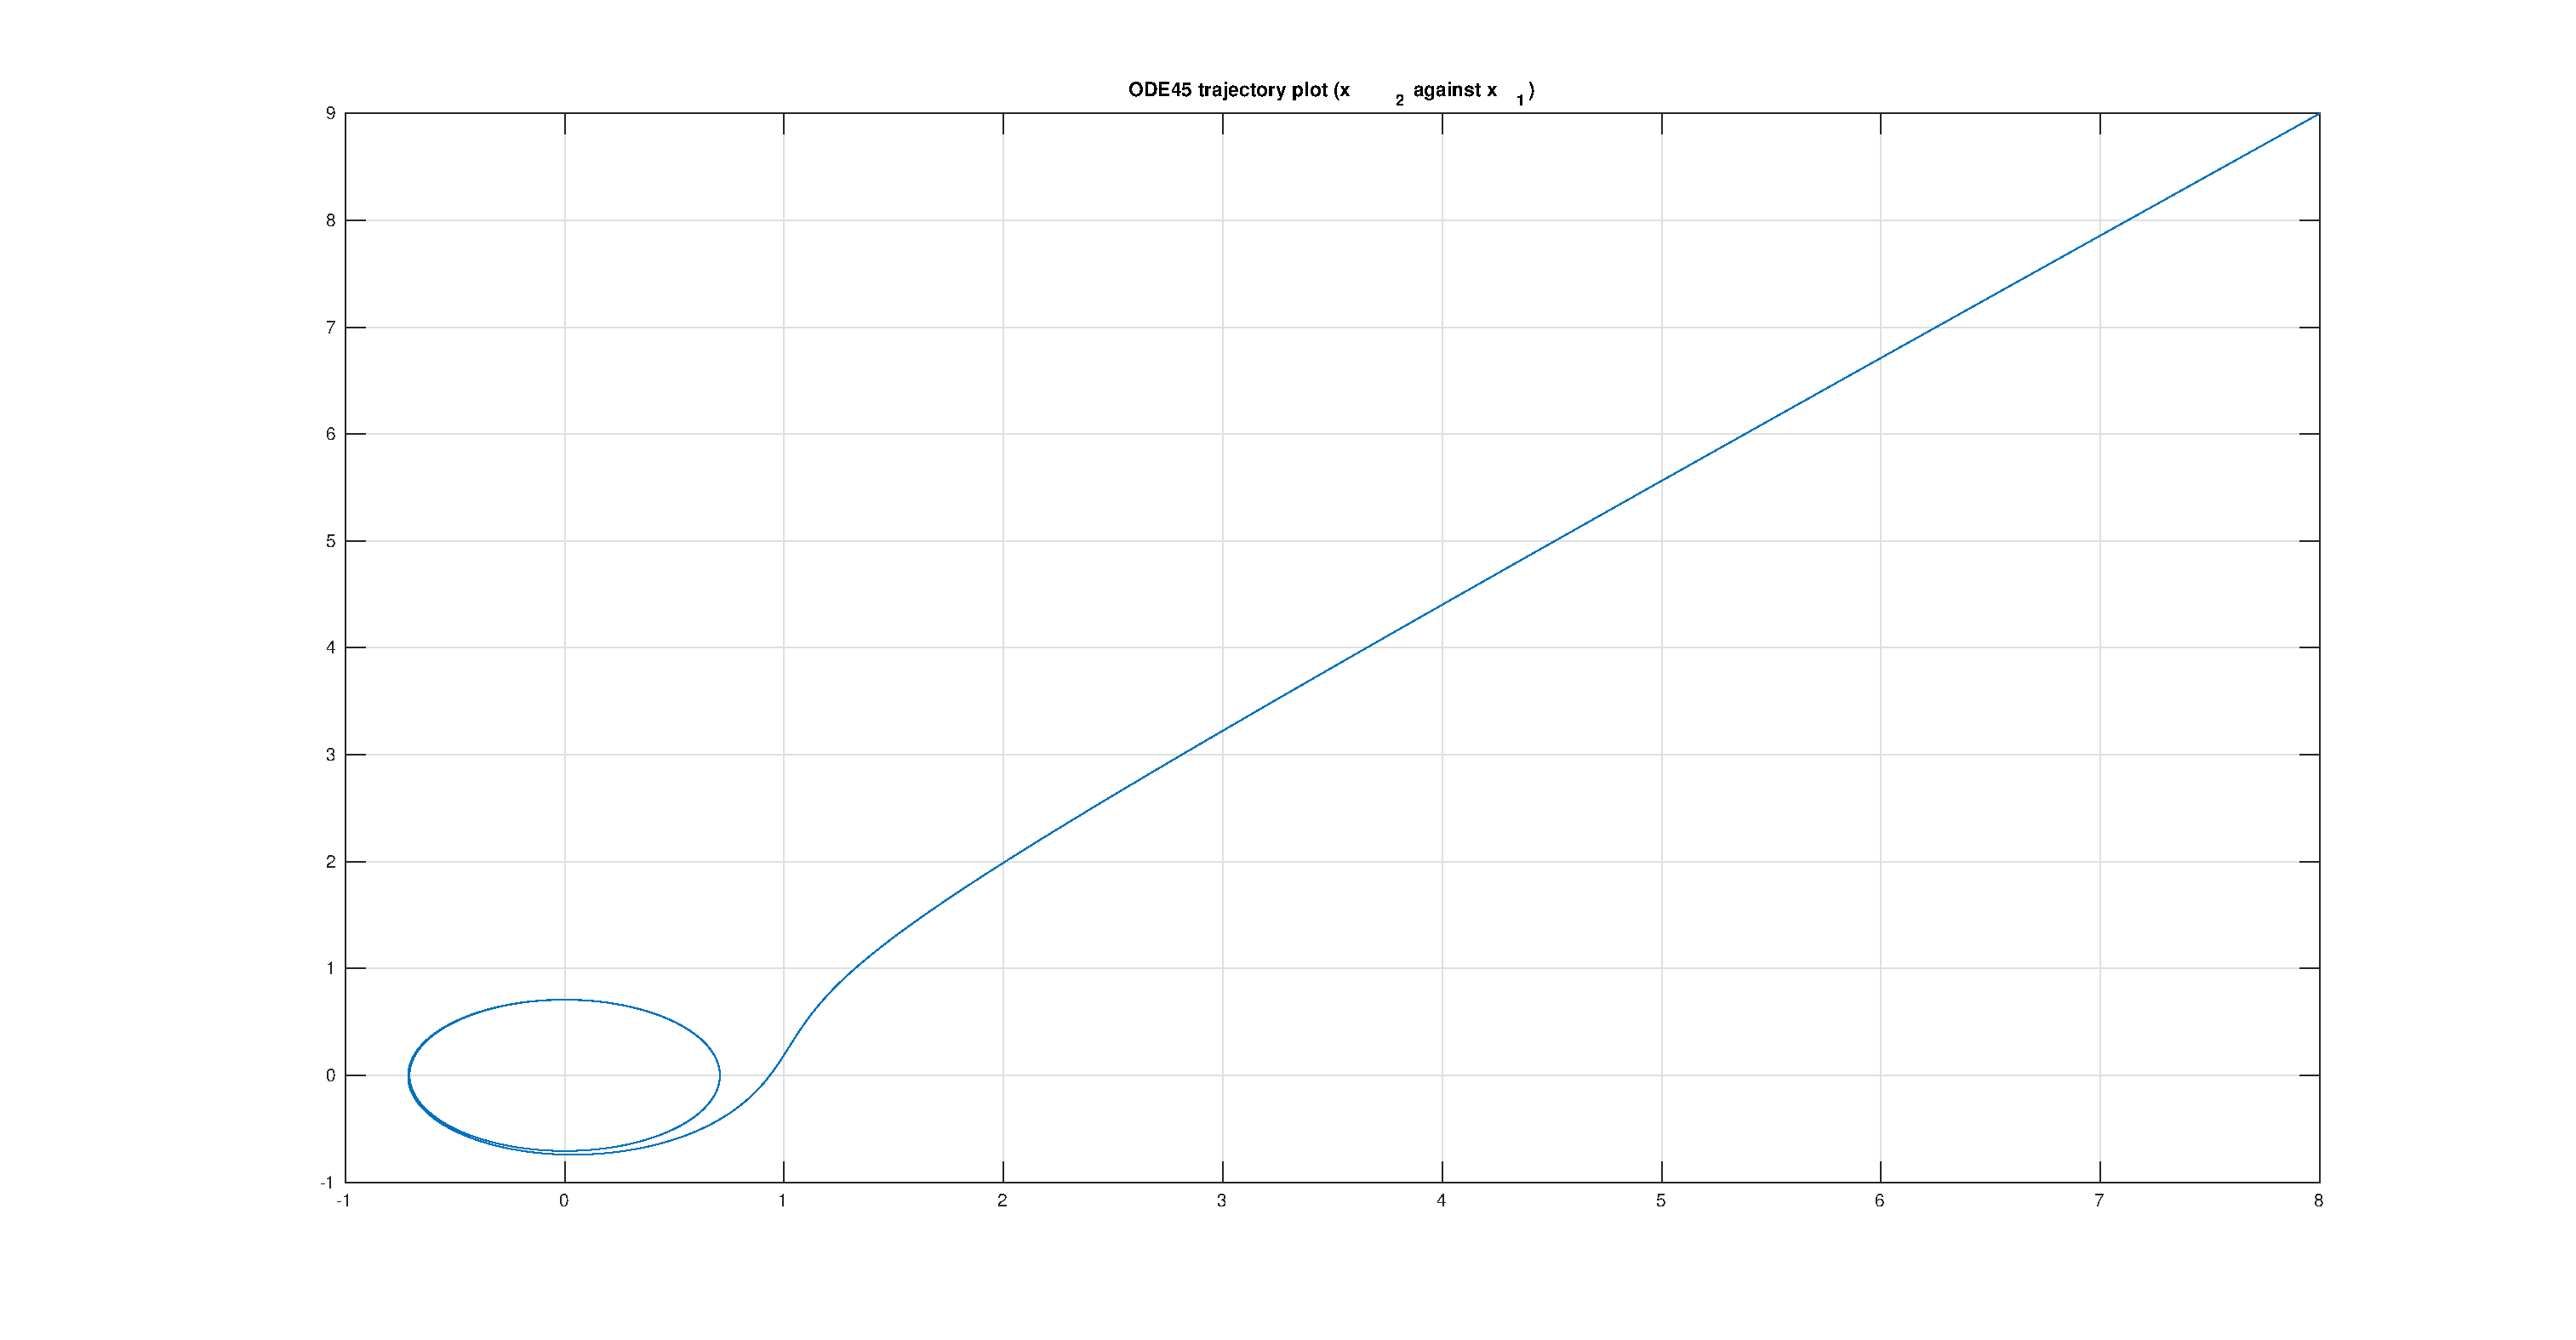
\includegraphics[scale=0.25]{29.eps}
\end{center}


\begin{thebibliography}{9}
\bibitem{texbook}
Piotr Tatjewski (2014) \emph{Numerical Methods}, Oficyna Wydawnicza Politechniki Warszawskiej
\end{thebibliography}


\end{document}
